\documentclass[ xcolor = pdftex, dvipsnames, table ]{beamer}

%one line dots
%\usetheme[compress]{Berlin}
%one line per subsection
\usetheme{Berlin}
\usecolortheme{whale}
\setlength{\parskip}{0.1in}
\usepackage{bm}
\usepackage{color}
\usepackage{graphicx}
\usepackage{xcolor}
\usepackage{tikz}
\usepackage{tabularx}
\usepackage{stackengine}
\usetikzlibrary{positioning, shapes, snakes}

%\usepackage{ctable}
%\usepackage[percent]{overpic}
%\usepackage[makeroom]{cancel}

\makeatletter
\def\hlinewd#1{
\noalign{\ifnum0=`}\fi\hrule \@height #1
\futurelet\reserve@a\@xhline}
\makeatother

\definecolor{inlinks}{HTML}{ 00008B }
\definecolor{outlinks}{HTML}{ 148F77 }
%\hypersetup{colorlinks,linkcolor=,urlcolor=links}
\hypersetup{
	colorlinks=false,
	linkbordercolor=inlinks,
	linkcolor=inlinks,	
	urlbordercolor=outlinks,
   	linkbordercolor=inlinks,
   	citebordercolor=inlinks,
   	menubordercolor=inlinks,
	%runbordercolor=inlinks,
   	%citebordercolor=inlinks,
   	%filebordercolor=inlinks,
	pdfborderstyle={/S/U/W 2}
}

%
%

\begin{document}
%
%ftp://ftp.pcouncil.org/pub/!!!Catch_Estimation_Methodology_Review_2018/

\title{\textbf{Improving Catch Estimation Methods in Sparsely Sampled, Mixed Stock Fisheries.}}

\author{
%\textbf{\mbox{Nick Grunloh}}
%%$~$\\
%%\vspace{-0.5cm}
\textbf{Nicholas Grunloh }\\\vspace{0.3cm}
\textbf{In Cooperation With:}\\
\textbf{E.J. Dick, Don Pearson, John Field, Marc Mangel}
}

\institute[]{\textbf{UCSC :: CSTAR :: SWFSC :: NMFS}}

\date{
%$~$\\
%\vspace{-1.5cm}
%\includegraphics[width=0.45\textwidth]{./Rockfish.png}\\
\textbf{31 July 2018}
}

%
%

%
\section{Introduction}
\subsection{}
\begin{frame}
        \maketitle
\end{frame}

%
%

%
\subsection{Diagnostic Tutorial}
\begin{frame}
\small
\textbf{Request:} 
As a diagnostic template, for each sampled stratum compare the posterior 
predictive distributions at the 68th, 95th, and 99th percentiles with the 
current observed species proportions (create fully stratified versions of 
tables 2 and 3 in the Grunloh et al. methods documentation).  With each row, 
include sample sizes and associated landing weights with a graphical display 
to highlight problems and outliers (circle size proportional to landing 
weights).
  
\textbf{Rationale:}  
The Team provided broad-scale summary metrics (e.g., MSE and DIC) for 
evaluating the goodness-of-fit of the different model forms and structures.  
Fine-scale diagnostics are needed to help identify aspects of the data that 
are not adequately addressed by the different models.  The diagnostic template 
will provide a mechanism for fine-scale exploration of goodness-of-fit.

\textbf{Response:}  
The following slides show the requested diagnostic plot and demonstrate how to 
maneuver as well as interpret them.

\end{frame}

%
%

%
\begin{frame}{Beta-Binomial Model}
\vspace{-0.5cm}
%\begin{align*}
\begin{equation*}
        y_{ijklm\eta} \sim \text{Beta-Binomial}\Big(\mu_{jklm\eta},~\sigma^2_{jklm\eta} \Big)
\end{equation*}
\vspace{-0.7cm}
\begin{gather*}
%       \vspace{0.2cm}
        \mu_{jklm\eta} = n~\text{logit}^{-1}(\theta_{jklm\eta})\\
        %=n~\frac{\alpha_{jklm\eta}}{\alpha_{jklm\eta}+\beta_{jklm\eta}}  
        \sigma^2_{jklm\eta} = \mu_{jklm\eta}\Big(1-\frac{\mu_{jklm\eta}}{n}\Big)\Big(1+(n-1)~\rho\Big)
        %\sigma^2_{jklm\eta} = \bigg(\mu_{jklm\eta}-\frac{\mu^2_{jklm\eta}}{n}\bigg)\bigg(1+(n-1)~\rho\bigg)
%       \vspace{0.2cm}
\end{gather*}
\vspace{-0.2cm}
\begin{equation*}
        \theta_{jklm\eta} = \beta_0 + \beta^{(s)}_j + \beta^{(p)}_k + \beta^{(g)}_l + \color{blue}{\beta^{(t)}_{m\eta}}%\beta^{(y)}_m + \beta^{(q)}_\eta +
% \beta^{(y:q)}_{m\eta}   %{\color{blue}a_{jklm\eta}} + {\color{OliveGreen}b_{jklm\eta}} %+ c^*_{jklm\eta}
        %=n~\text{logit}^{-1}(\theta_{jklm\eta})
\end{equation*}
\hspace{-0.5cm}
%0.68
\begin{minipage}[h!]{0.55\textwidth}
        $~$\\
        $y_{ijklm\eta}$: $i^{\text{th}}$ sample of the $j^{\text{th}}$ species' integer weight, in the $k^{\text{th}}$ port, caught with the $l^{\text{th}}$ gear, in the $\eta^{\text{th}}$ \mbox{quarter,} of year $m$, for a particular market \mbox{category.}
\end{minipage}
\begin{minipage}{0.45\textwidth}
        \vspace{-0.5cm}
        \hspace{4cm}
        \begin{eqnarray*}
        j &\in&\left\{1, ..., J\right\} \text{Species}\\
        k &\in&\left\{1, ..., K\right\} \text{Ports}\\
        l &\in&\left\{1, ..., L\right\} \text{Gears}\\
        m &\in&\left\{1, ..., M\right\} \text{Years}\\
        \eta &\in&\left\{1, ..., H\right\} \text{Quarters}
        \end{eqnarray*}
\end{minipage}
\end{frame}



%%
%\begin{frame}{Likelihood}
%	
%\end{frame}

%
%

%
\begin{frame}%{Information Criterion}
\begin{minipage}{0.49\textwidth}
\hspace*{3cm}
\begin{table}[ht!]
        \centering
        \begin{tabular}[c]{@{}lcccccc@{}}
        %\toprule
        \hline
        & \href{https://github.com/gasduster99/sppComp/tree/master/sscRuns/25019781982M4}{M4} \\ \hline 
	DIC & 38721 \\
	WAIC & 38725 \\ \hline
        \end{tabular}
\end{table}
\begin{center}
\textbf{(M4)}
\begin{eqnarray*}
&\beta^{(t)}_{m\eta} = \beta^{(y:q)}_{m\eta}&\\
&\beta^{(y:q)}_{m\eta} \sim N(0, v)&\\
&~&
\end{eqnarray*}
\end{center}
\end{minipage}
\begin{minipage}{0.49\textwidth}
$~$\\$~$\\
\hspace*{-3cm}
\begin{itemize}
\item[$\leftarrow~$ click $~$] Text \underline{underlined} in {\color{outlinks}green} links to the appropriate diagnostics for all species and stratum.
\item species-port-gear-year-qtr, species-gear-year, species-year
\item disaggregated*.csv, gearYearSpp*.csv, yearSpp*.csv
\item marginal plots by species
\end{itemize}
\end{minipage}
\end{frame}

%
%

%
\begin{frame}{MAD Diagnostic}
Let $\ell_i$ be the landings in stratum $i$, $\mathcal{O}_{ij}$ be the observed 
predictive accuracy of species $j$ in stratum $i$, and $\aleph$ be the nominal level of 
prediction for a particular model run. The Mean Absolute Deviation (MAD) for species 
$j$ in stratum $i$ is 
	\begin{equation*} %abs(coverage-level) * landing/sum(landing)
		\text{MAD}_{ij} = \frac{\ell_i}{\sum_i \ell_i}\left| \mathcal{O}_{ij}-\aleph \right|.
	\end{equation*}
\begin{itemize}
\item Low MAD scores occur when $\ell_i$ is low -or- $\left|\mathcal{O}_{ij}-\aleph\right|$ is small.
%the observed predictive accuracy ($\mathcal{O}_{ij}$) is very near the nominal level of prediction ($\aleph$).

\item High MAD scores occur when $\ell_i$ is large and $\left|\mathcal{O}_{ij}-\aleph\right|$ is large.

\item Thus high MAD scores represent important mistakes, and low MAD scores 
represent either unimportant mistakes, or important correctness :) 

\end{itemize}
\end{frame}

%
%

%
\begin{frame}{Stratum Plots}
	We show predictive accuracy at three levels of stratification: 
	\begin{itemize}
	\item \href{https://github.com/gasduster99/sppComp/tree/master/sscRuns/25019781982M4/species-port-gear-year-qtr/}{species-port-gear-year-qtr} is fully disaggregated predictions.
	\item \href{https://github.com/gasduster99/sppComp/tree/master/sscRuns/25019781982M4/species-gear-year/}{species-gear-year} marginalizes over port and quarter; showing marginalized predictions by species, gear, and year.
	\item \href{https://github.com/gasduster99/sppComp/tree/master/sscRuns/25019781982M4/species-year/}{species-year} marginalizes over port, quarter, and gear; showing marginalized predictions by species and year.
	\end{itemize} 
	In each run's directory (\href{https://github.com/gasduster99/sppComp/tree/master/sscRuns/25019781982M4}{here} is M4's) disaggregated*.csv, gearYearSpp*.csv, yearSpp*.csv are csv versions of these images. 
\end{frame}

%
%

%
\begin{frame}%{Marginal Plot}

\begin{minipage}{0.39\textwidth}
	\begin{figure}[ht!]
	\vspace*{-0.5cm}
        \hspace*{-1cm}	
	\includegraphics[height=1.1\textheight]{{../sscRuns/25019781982M4/margCNRY/margCNRY-0.68-Diagnostic}.pdf}
        \end{figure}
\end{minipage}
\begin{minipage}{0.59\textwidth}
\begin{itemize}
	\item Marginal Plots condition on a single species (CNRY here).
	\item For a particular species, each row conditions on a single stratum and marginalizes over all other strata.
	\item Use:
	\begin{itemize}
		\item Sort species by MAD score.
		\item Given a particular species, explore margins via marginal plots.
		\item Explore within the margins via the previously described stratum plots.
	\end{itemize} 
\end{itemize}
\end{minipage}
\end{frame}

%
%

%
\subsection{}
\begin{frame}
\small
\textbf{Request:}
Provide a summary table of species’ sample sizes in each market category by 
time block.

\textbf{Rationale:}
The requested information will assist in understanding where there are gaps in 
the available data that the model is filling in by means of its pooling 
structure.

\textbf{Response:} 
The following slides show tables of total sample sizes and the frequency of 
occurrence by species within each sample (across all years, gears, ports and 
quarters within a time period) for the three rockfish market categories that 
we focus on in the presentation, as well as elasmobranchs and flatfish.  
Supplementary excel files include data summaries and pivot tables that can be 
used to review the same information for all other market categories, as well 
as these and other market categories at higher levels of stratification (year, 
port complex, gear, quarter) to address specific questions or concerns. 

\end{frame}

%
%

%
\begin{frame}
\hspace*{-0.5cm}
\begin{minipage}{0.29\textwidth}
\small
This table shows the total number of samples for Market Category 250 
(Unspecified rockfish) in five major time periods. 
%(noting that this market 
%category was among the most heavily used early, but lightly used in later time 
%periods; see Figure 2 of Grunloh et al. report from first review- I’d like to 
%add total catches for this MC and time period to upper row of table!)
The sparseness of some species in the sample data (e.g., bronzespotted rockfish in 
the 1978-1982 period, when just one was encountered) directly relates to the 
challenges and poor diagnostics in the fits for such rare species.   
\end{minipage}
\begin{minipage}{0.69\textwidth}
	\hspace*{0.5cm}
	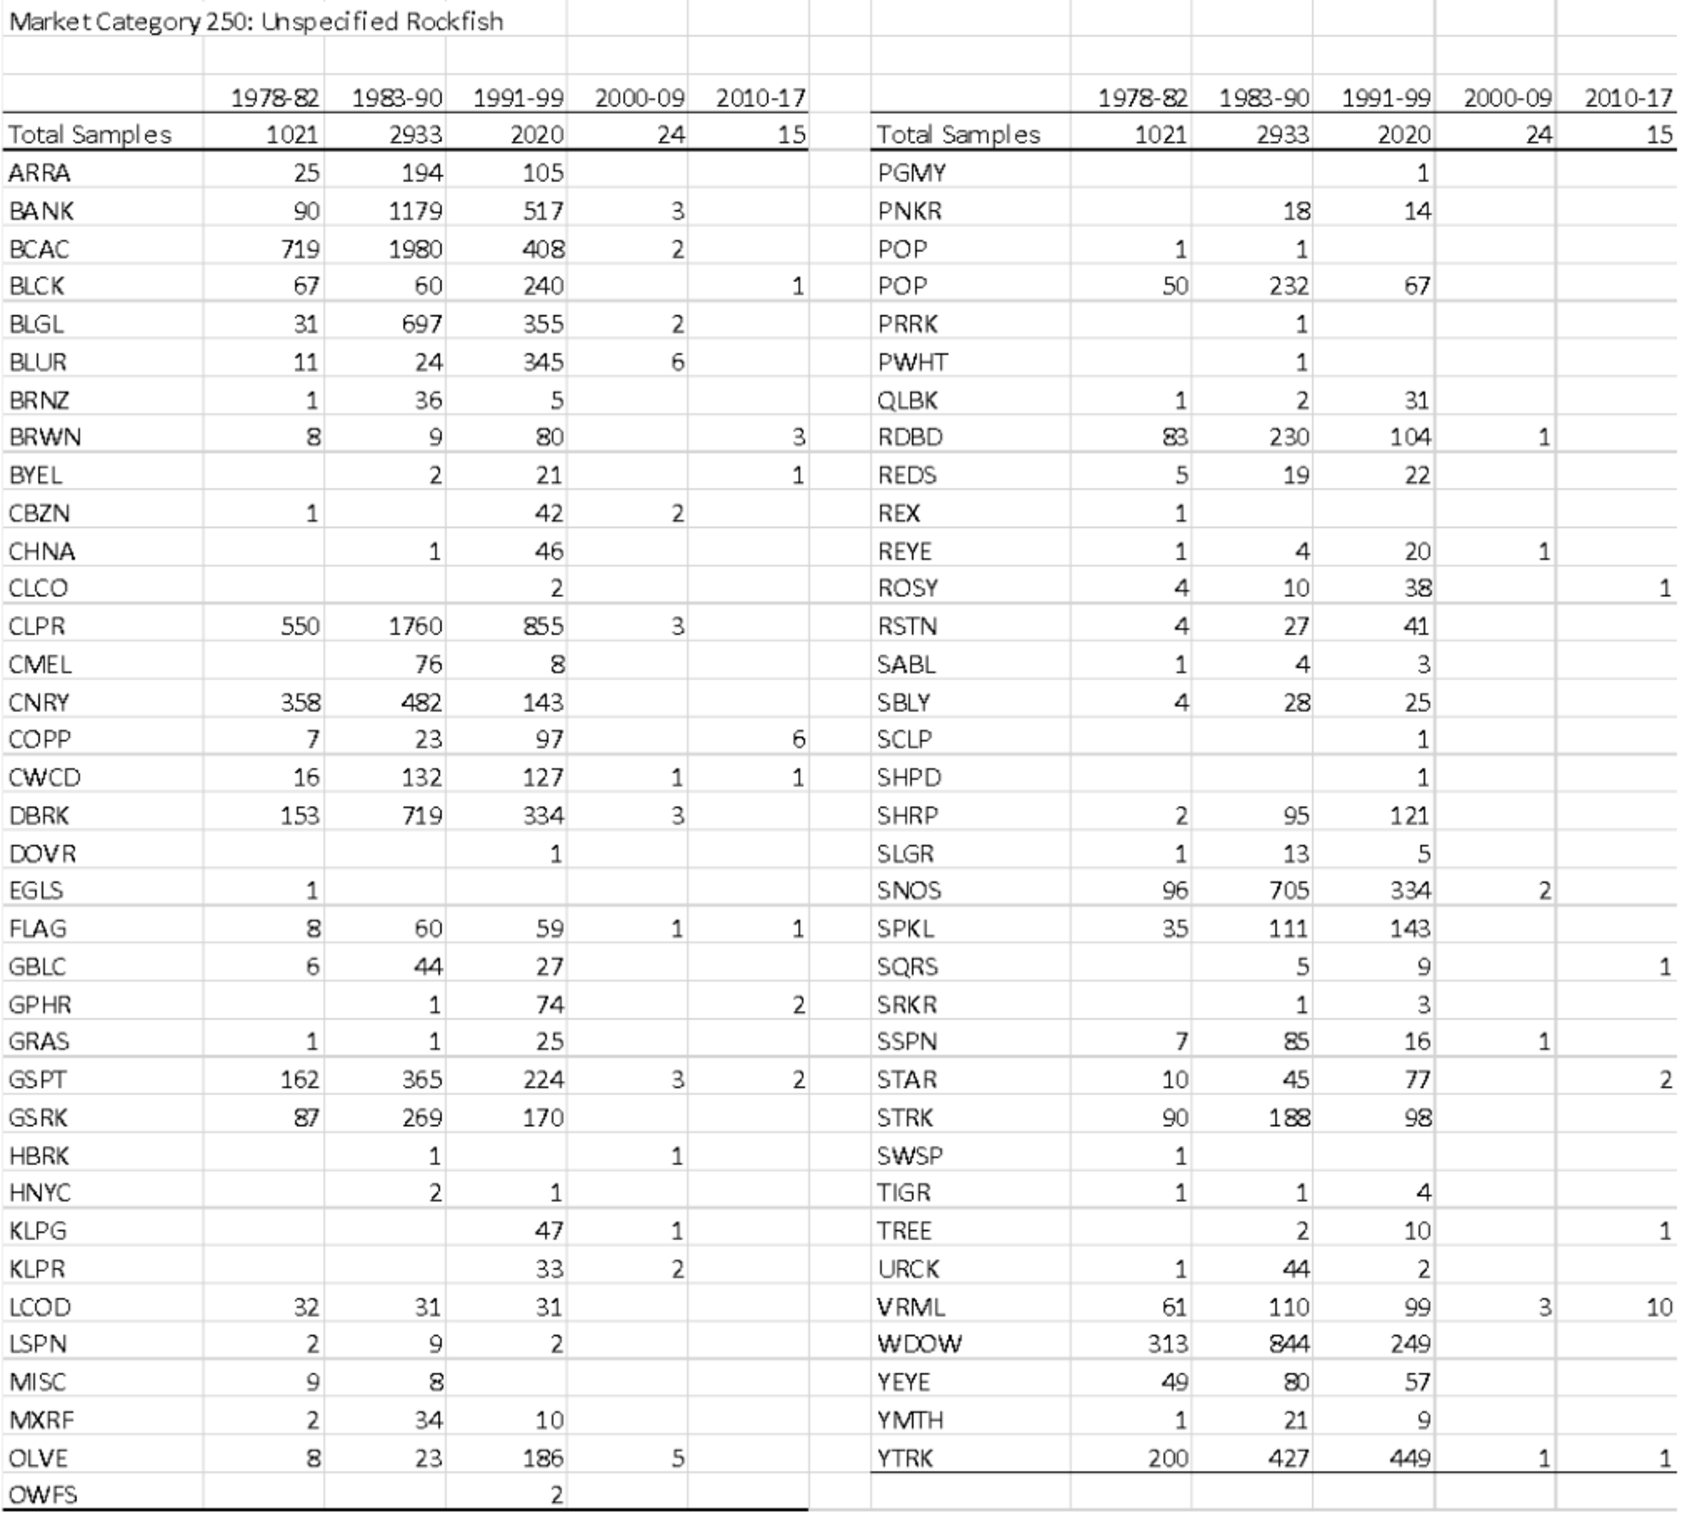
\includegraphics[height=1\textheight]{./pictures/sampleTable250.pdf} 
\end{minipage}
\end{frame}

%
%

%
\begin{frame}
\hspace*{-0.5cm}
\begin{minipage}{0.39\textwidth}
These tables show the total number of samples for Market Category 253 
(Bocaccio) and 269 (Widow rockfish), with the frequency of occurrence of all 
other rockfish species in each sample, in five major time periods.
\end{minipage}
\begin{minipage}{0.59\textwidth}
	\hspace*{0.5cm}
	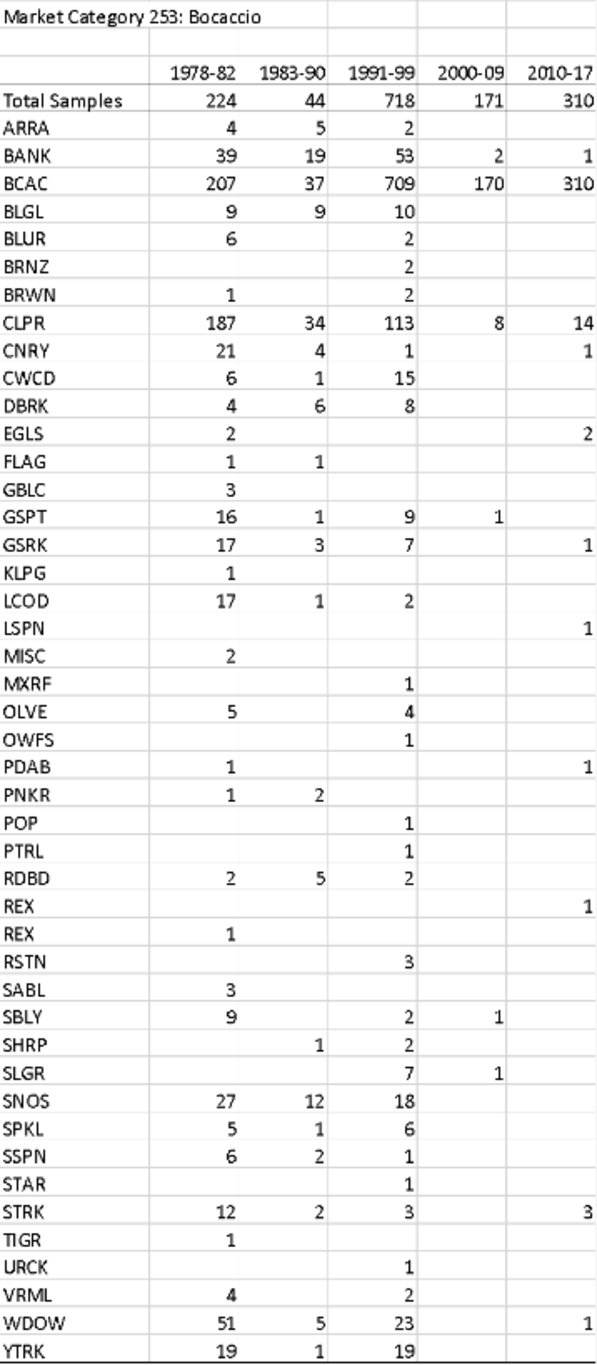
\includegraphics[width=0.5\textwidth]{./pictures/sampleTable253.pdf}
	%\vspace*{-0.5cm}
	\hspace*{0.3cm}
	\raisebox{0.2\height}{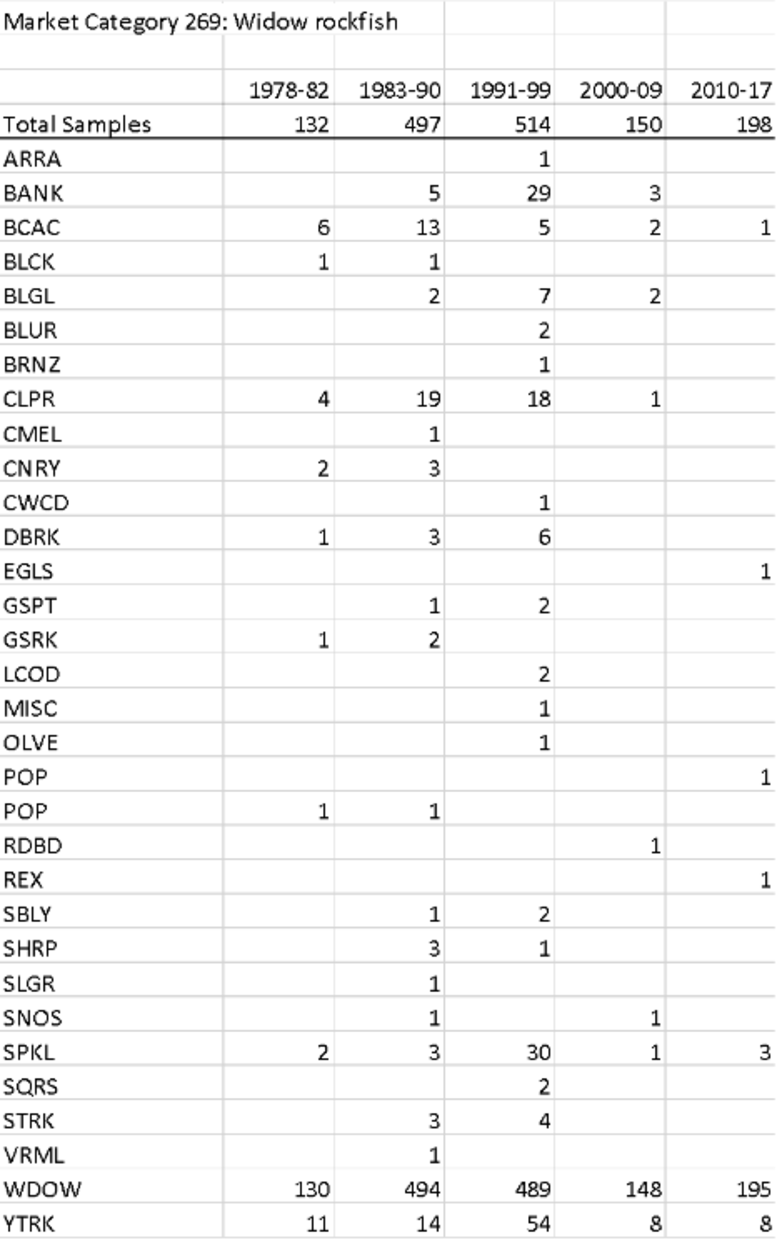
\includegraphics[width=0.53\textwidth]{./pictures/sampleTable269.pdf}}
	%\vspace{5cm}
\end{minipage}
\end{frame}

%
%

%
\begin{frame}
%\hspace*{-0.5cm}
%\begin{minipage}{0.29\textwidth}
%%\footnotesize
%\scriptsize
Moving beyond rockfish into flatfish and elasmobranch (primarily skates) market 
categories, these tables shows the total number of samples and frequency of occurrence 
by species for the largest flatfish (table on left and elasmobranch (table on right) 
market categories.  Flatfish species composition data have only been collected since 
2002, and elasmobranchs since 2009, so all years are combined here (and information at 
higher stratification levels, including more sparsely sampled market categories, are 
available in the excel file). 
%\end{minipage}
%\begin{minipage}{0.69\textwidth}
%	\vspace{-1cm}
%	%\hspace*{-0.5cm}
%	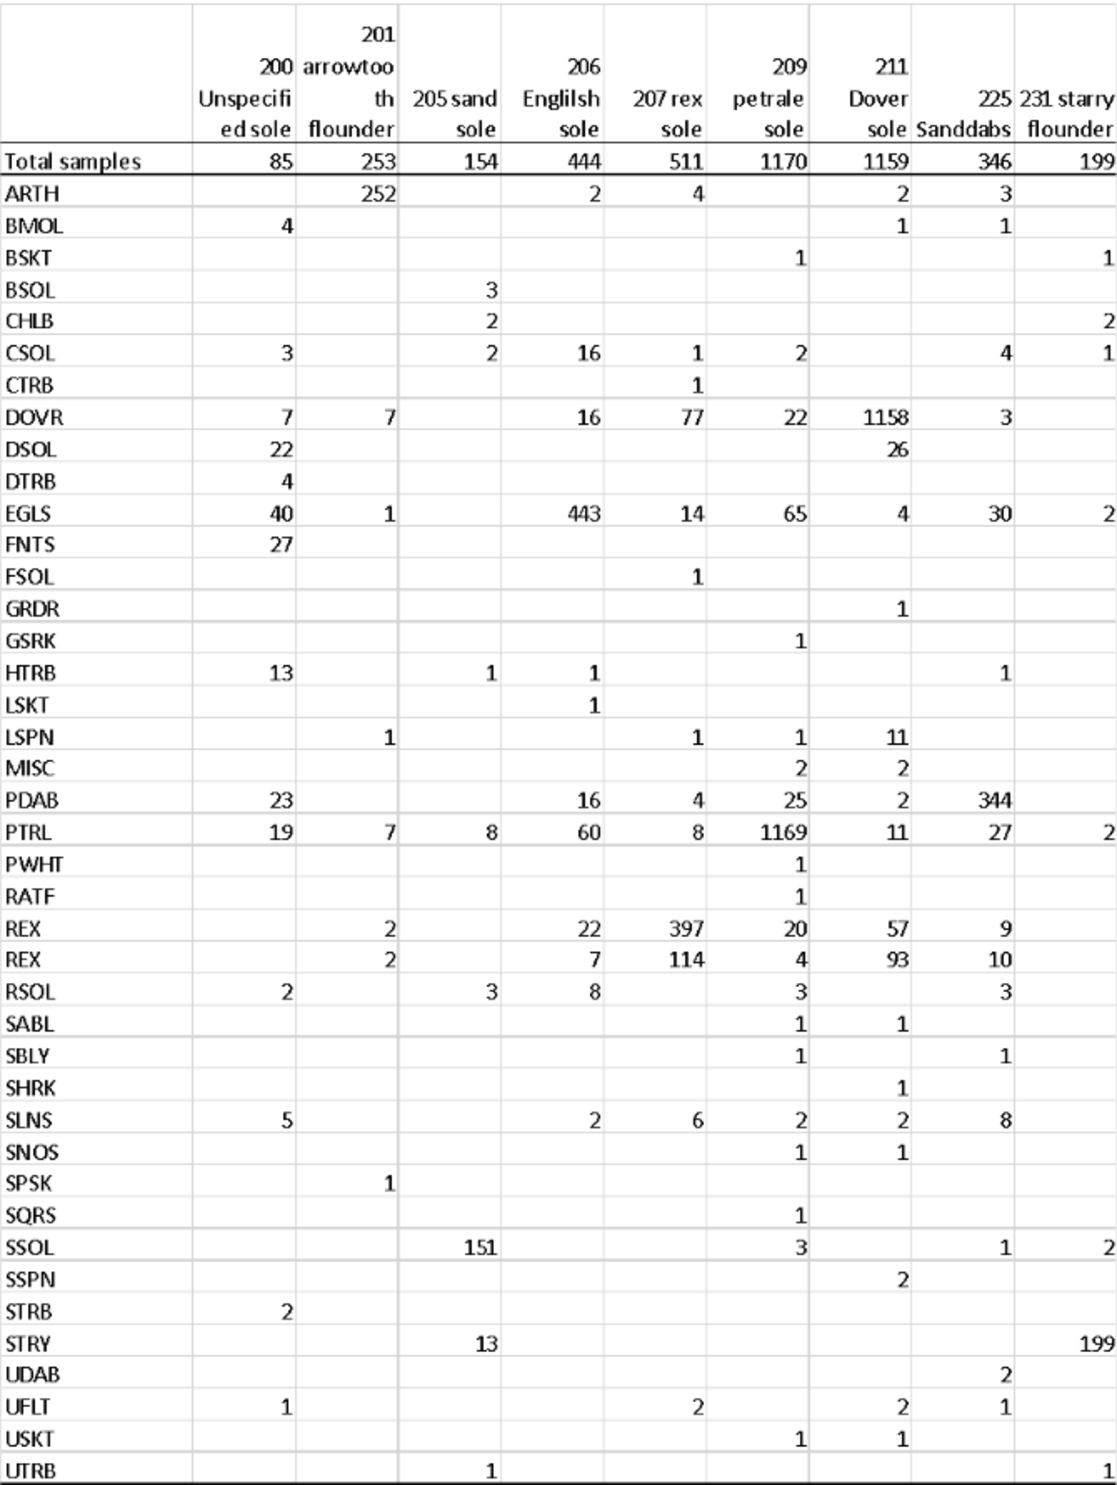
\includegraphics[width=0.55\textwidth]{./pictures/sampleTableFlat.pdf}
%	%\vspace*{-0.5cm}
%	\hspace*{0.3cm}
%	\raisebox{0.2\height}{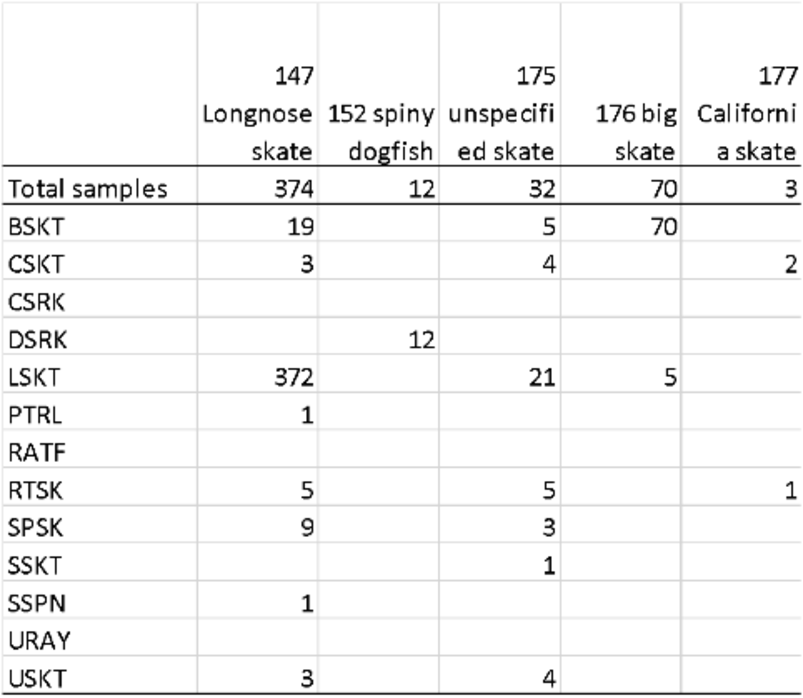
\includegraphics[width=0.53\textwidth]{./pictures/sampleTableElas.pdf}}
%	%\vspace{5cm}
%\end{minipage}
\end{frame}

%
%

%
\begin{frame}
%\hspace*{-0.5cm}
%\begin{minipage}{0.29\textwidth}
%%\footnotesize
%\scriptsize
%Moving beyond rockfish into flatfish and elasmobranch (primarily skates) market 
%categories, these tables shows the total number of samples and frequency of occurrence 
%by species for the largest flatfish (table on left and elasmobranch (table on right) 
%market categories.  Flatfish species composition data have only been collected since 
%2002, and elasmobranchs since 2009, so all years are combined here (and information at 
%higher stratification levels, including more sparsely sampled market categories, are 
%available in the excel file). 
%\end{minipage}
%\begin{minipage}{0.69\textwidth}
%	\vspace{-1cm}
	\hspace*{-0.5cm}
	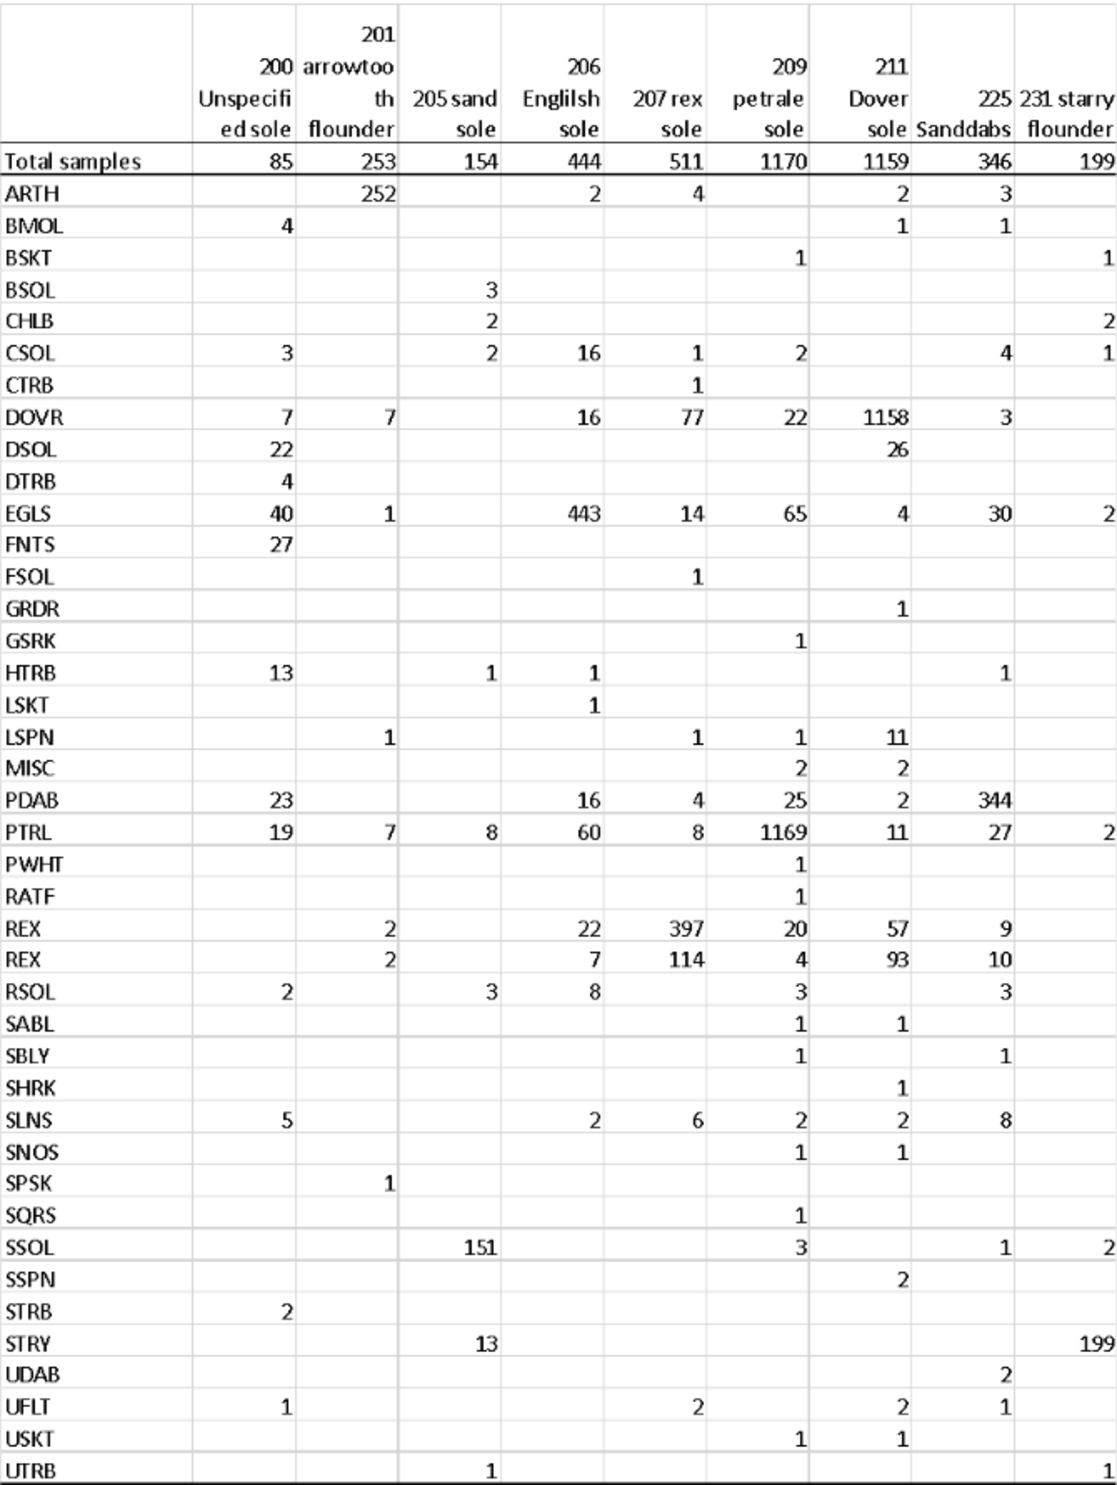
\includegraphics[width=0.5\textwidth]{./pictures/sampleTableFlat.pdf}
%	%\vspace*{-0.5cm}
	\hspace*{0.3cm}
	\raisebox{0.2\height}{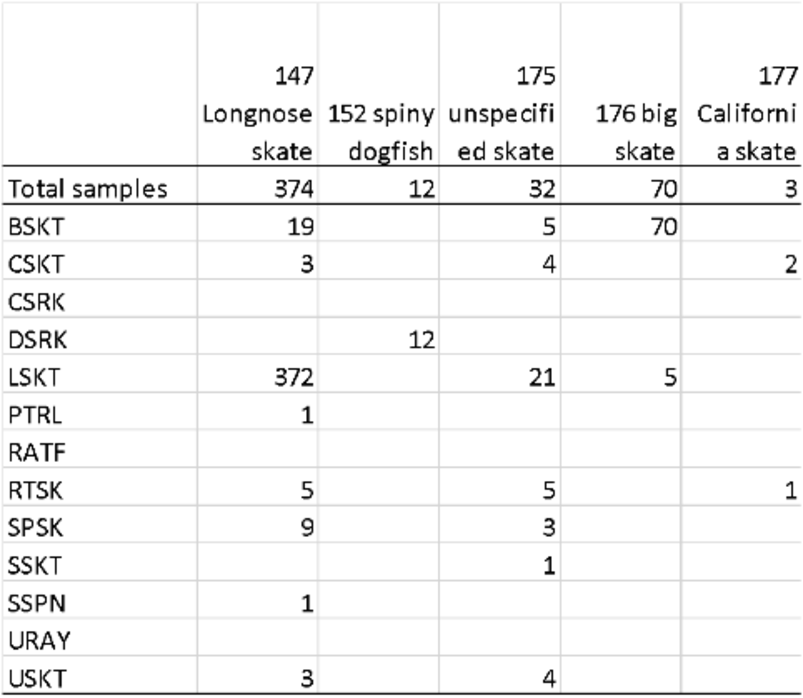
\includegraphics[width=0.53\textwidth]{./pictures/sampleTableElas.pdf}}
%	%\vspace{5cm}
%\end{minipage}
\end{frame}



%
\subsection{}
\begin{frame}
\textbf{Request:}
Redo the modeling of the early time block without southern CA ports. Explore 
spatially and temporally (i.e., alternative time blocks).

\textbf{Rationale:}
The available dataset does not have any sample data in the early time block 
from the southern CA ports. It was unclear how this lack of data influenced 
the model results. The requested analysis will clarify the situation.

\textbf{Response:}
All of the model runs and plots from this point forward only model ports 
north of point conception. 

\end{frame}

%
%

%
\section{Time Model}
\subsection{}
%

%
%

\begin{frame}
\textbf{Request:}
The diagnostic template should be developed for each of the sensitivity runs 
(vary across a range of plausible time models and priors and limit to the top 
2-3 market categories).  

\textbf{Rationale:}
Application of the diagnostics across a wide range of models will form a test 
of how well the diagnostics illustrate whether the models capture important 
structural features that are thought to be embedded in the data.

\textbf{Response:}
The following slides show the requested diagnostic plots as applied to models 
across a range of time models and prior choices.

\end{frame}

%
%

%
\begin{frame}{Time Models}
\hspace*{-0.5cm}
\begin{minipage}{0.3\textwidth}
\begin{center}
\textbf{(M1)}
\begin{eqnarray*}
&\beta^{(t)}_{m\eta} = \beta^{(y)}_{m} + \beta^{(q)}_{\eta}&\\
&\beta^{(y)}_{m} \sim N(0, 32^2)&\\
&\beta^{(q)}_{\eta} \sim N(0, 32^2)&\\
&~&
\end{eqnarray*}
\end{center}

\begin{center}
\textbf{(M4)}
\begin{eqnarray*}
&\beta^{(t)}_{m\eta} = \beta^{(y:q)}_{m\eta}&\\
&\beta^{(y:q)}_{m\eta} \sim N(0, v)&\\
&~&
\end{eqnarray*}
\end{center}
\end{minipage}
\begin{minipage}{0.3\textwidth}
\begin{center}
\textbf{(M2)}
\begin{eqnarray*}
&\beta^{(t)}_{m\eta} = \beta^{(y)}_{m} + \beta^{(q)}_{\eta}&\\
&\beta^{(y)}_{m} \sim N(0, v^{(y)})&\\
&\beta^{(q)}_{\eta} \sim N(0, v^{(q)})&\\
&~&
\end{eqnarray*}
\end{center}

\begin{center}
\textbf{(M5)}
\begin{eqnarray*}
&\beta^{(t)}_{m\eta} = \beta^{(y:q)}_{m\eta}&\\
&\beta^{(y:q)}_{m\eta} \sim N(0, v_\eta)&\\
&~&
\end{eqnarray*}
\end{center}
\end{minipage}
%\vspace*{-1cm}
\begin{minipage}{0.3\textwidth}
\begin{center}
~~~~~~~~~~~~~\textbf{(M3)}
\begin{eqnarray*}
&\beta^{(t)}_{m\eta} = \beta^{(y)}_{m} + \beta^{(q)}_{\eta} + \beta^{(y:q)}_{m\eta} & \\
&\beta^{(y)}_{m} \sim N(0, v^{(y)}) & \\
&\beta^{(q)}_{\eta} \sim N(0, v^{(q)}) & \\
&\beta^{(y:q)}_{m\eta} \sim N(0, v) &
\end{eqnarray*}
\end{center}

\begin{center}
\textbf{(M6)}
\begin{eqnarray*}
&\beta^{(t)}_{m\eta} = \beta^{(y:q)}_{m\eta}&\\
&\beta^{(y:q)}_{m\eta} \sim N(0, v_m)&\\
&&
\end{eqnarray*}
\end{center}
\end{minipage}
\end{frame}

%
%

\subsection{MCAT 250}
\begin{frame}{}
	\begin{table}[ht!]
        \centering
        \begin{tabular}[c]{@{}lcccccc@{}}
        %\toprule
        \hline
        & \href{https://github.com/gasduster99/sppComp/tree/master/sscRuns/25019781982M1}{M1} & \href{https://github.com/gasduster99/sppComp/tree/master/sscRuns/25019781982M2}{M2} & \href{https://github.com/gasduster99/sppComp/tree/master/sscRuns/25019781982M3}{M3} & \href{https://github.com/gasduster99/sppComp/tree/master/sscRuns/25019781982M4}{M4} & \href{https://github.com/gasduster99/sppComp/tree/master/sscRuns/25019781982M5}{M5} & \href{https://github.com/gasduster99/sppComp/tree/master/sscRuns/25019781982M6}{M6} \\ \hline
        \(\Delta\) DIC & 6448.98 & 0.33 & 0 & 4.45 & 9.3 & 7.42 \\
        \(\Delta\) WAIC & 6421.5 & 0.37 & 0 & 4.52 & 8.25 & 6.55 \\ \hline
        %\(pr(M|y)\) & 0 & 0 & 0 & 0.03 & 0 & 0.97 \\ \hline
        \end{tabular}
        \end{table}
\end{frame}

%
%

\begin{frame}{$~~~~~~~~~~$ \href{https://github.com/gasduster99/sppComp/tree/master/sscRuns/25019781982M2}{M2} $~~~~~~~~~~~~~~~~~~~~$ \href{https://github.com/gasduster99/sppComp/tree/master/sscRuns/25019781982M3}{M3} $~~~~~~~~~~~~~~~~~~~~$ \href{https://github.com/gasduster99/sppComp/tree/master/sscRuns/25019781982M4}{M4} }	
	\begin{figure}[ht!]
        \centering
	\hspace*{-1cm}
        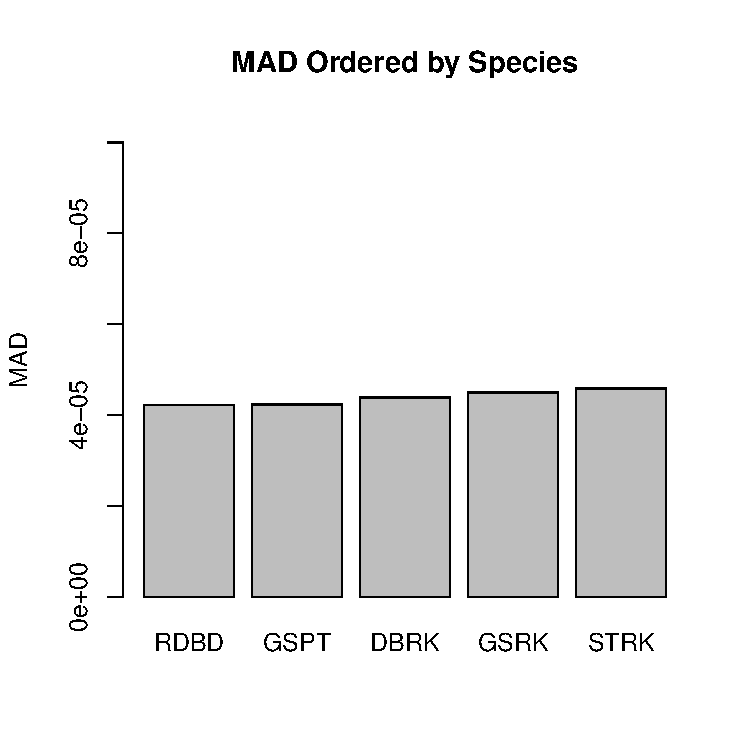
\includegraphics[width=.4\textwidth]{../sscRuns/25019781982M2/sppHeadMad68.pdf}
        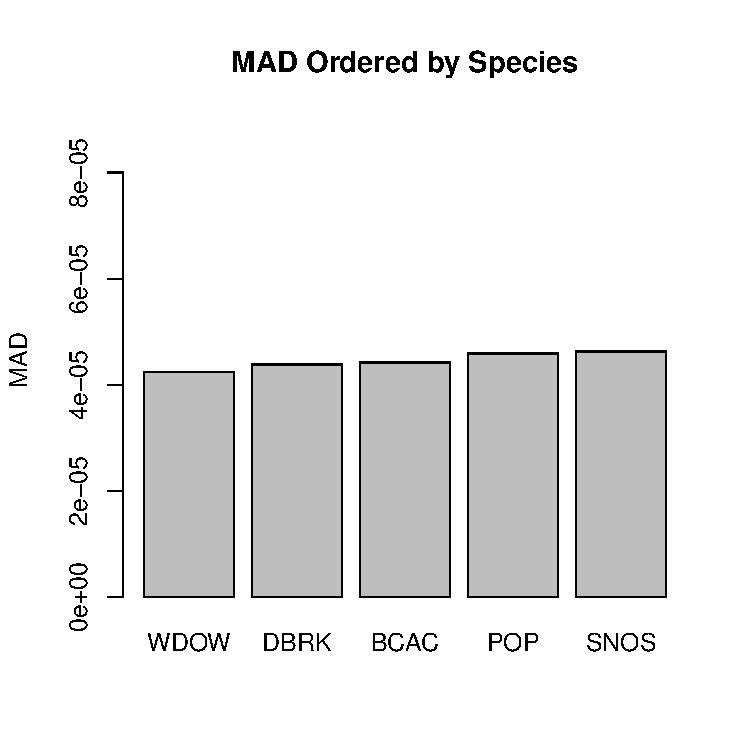
\includegraphics[width=.4\textwidth]{../sscRuns/25019781982M3/sppHeadMad68.pdf}
	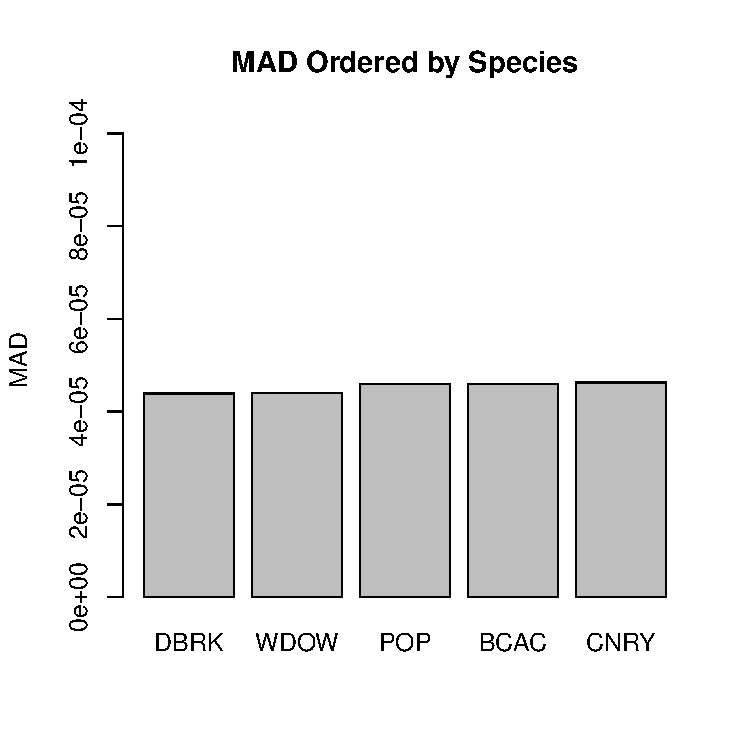
\includegraphics[width=.4\textwidth]{../sscRuns/25019781982M4/sppHeadMad68.pdf}
	\end{figure}
	\vspace{-1cm}
	\begin{center}
	\Large
	\href{https://github.com/gasduster99/sppComp/tree/master/try1/postSSC/25019781982M2M3M4}{Combined}
	\end{center}
\end{frame}

%
%

%
\begin{frame}
        \begin{figure}[ht!]
        \centering
        \vspace{-0.75cm}
        \includegraphics[height=1.1\textheight]{{./postSSC/25019781982M2M3M4/margBCAC/margBCAC-0.68-Diagnostic}.pdf}
        \end{figure}	
\end{frame}

%
%

%
\begin{frame}
	\begin{figure}[ht!]
        \centering
	\vspace{-0.75cm}
	%\begin{minipage}[h!]{0.49\textwidth}
	%\hspace*{-1cm}
        %\includegraphics[height=1.05\textheight]{{./postSSC/25019781982M2M3M4/margBCAC/margBCAC-0.68-Diagnostic}.pdf}
	%\end{minipage}
	%\begin{minipage}[h!]{0.49\textwidth}
	\includegraphics[height=1.1\textheight]{{./postSSC/25019781982M2M3M4/margWDOW/margWDOW-0.68-Diagnostic}.pdf}
	%\end{minipage}
        \end{figure}
\end{frame}

%
%

\begin{frame}{$~~~~~~~~~~$ \href{https://github.com/gasduster99/sppComp/tree/master/sscRuns/25019781982M2}{M2} $~~~~~~~~~~~~~~~~~~~~$ \href{https://github.com/gasduster99/sppComp/tree/master/sscRuns/25019781982M3}{M3} $~~~~~~~~~~~~~~~~~~~~$ \href{https://github.com/gasduster99/sppComp/tree/master/sscRuns/25019781982M4}{M4} }	
	\begin{figure}[ht!]
        \centering
	\hspace*{-1cm}
        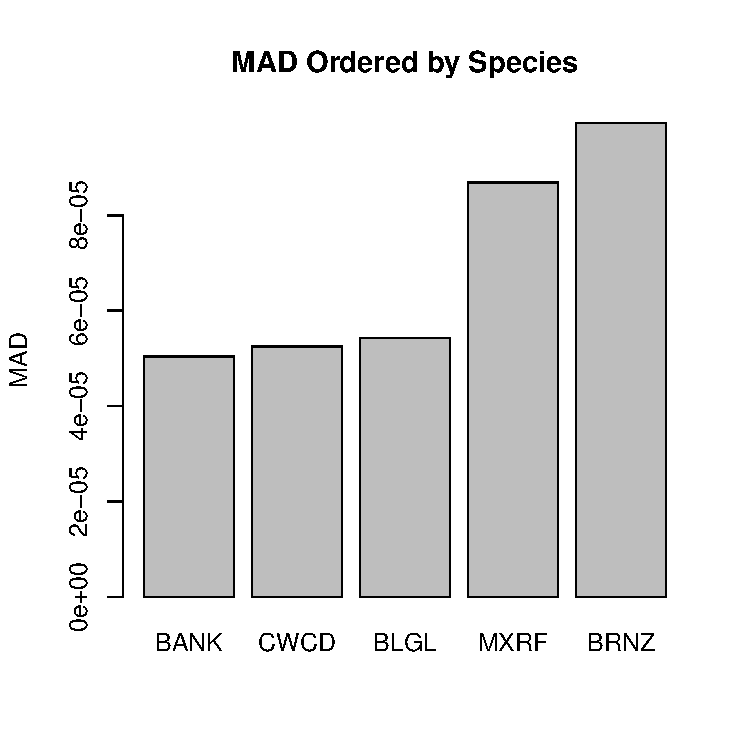
\includegraphics[width=.4\textwidth]{../sscRuns/25019781982M2/sppTailMad68.pdf}
        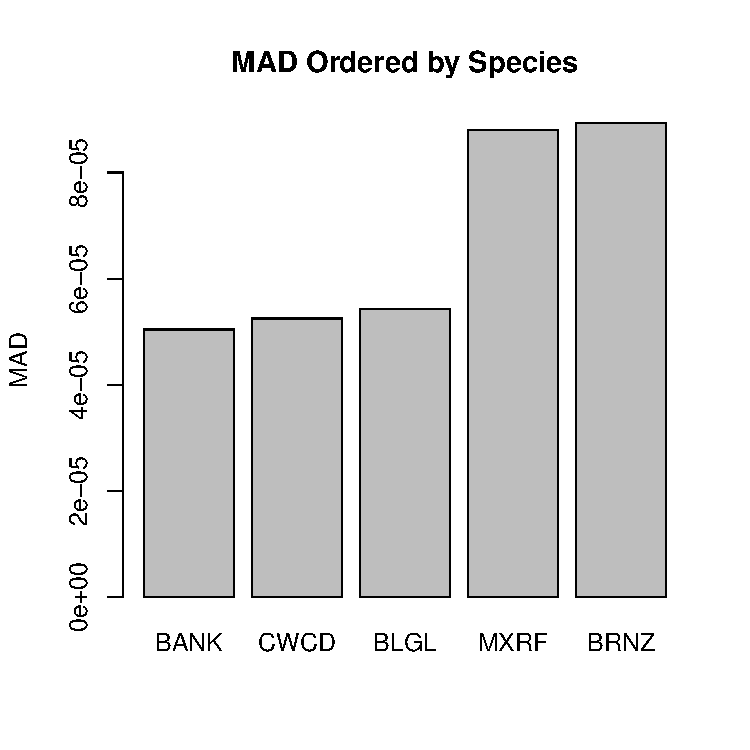
\includegraphics[width=.4\textwidth]{../sscRuns/25019781982M3/sppTailMad68.pdf}
	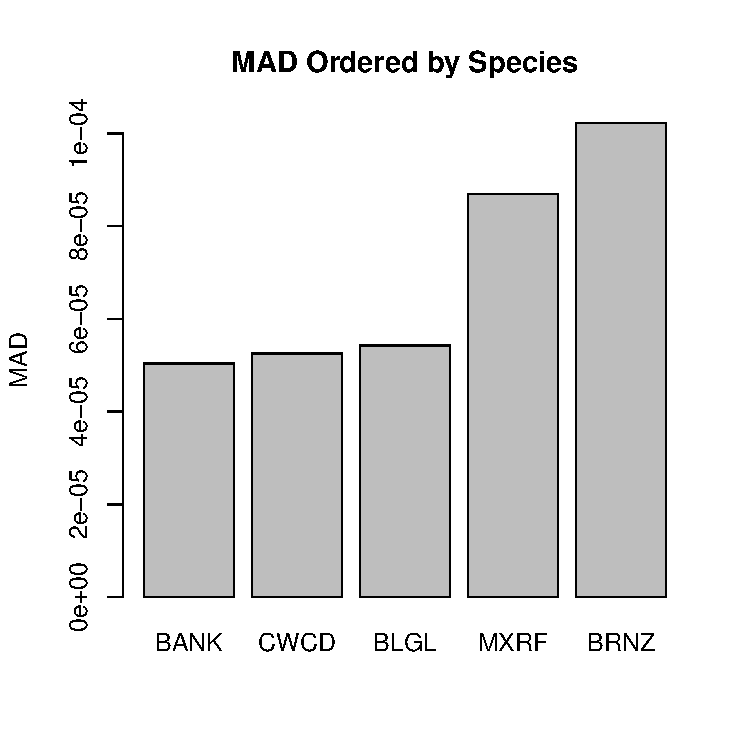
\includegraphics[width=.4\textwidth]{../sscRuns/25019781982M4/sppTailMad68.pdf}
	\end{figure}
	\vspace{-1cm}
	\begin{center}
	\Large
	\href{https://github.com/gasduster99/sppComp/tree/master/try1/postSSC/25019781982M2M3M4}{Combined}
	\end{center}
\end{frame}

%
%

%
\begin{frame}
        \begin{figure}[ht!]
        \centering
        \vspace{-0.75cm}
        \includegraphics[height=1.1\textheight]{{./postSSC/25019781982M2M3M4/margCWCD/margCWCD-0.68-Diagnostic}.pdf}
        \end{figure}    
\end{frame}

%
%

%
\begin{frame}
        \begin{figure}[ht!]
        \centering
        \vspace{-0.75cm}
        %\begin{minipage}[h!]{0.49\textwidth}
        %\hspace*{-1cm}
        %\includegraphics[height=1.05\textheight]{{./postSSC/25019781982M2M3M4/margBCAC/margBCAC-0.68-Diagnostic}.pdf}
        %\end{minipage}
        %\begin{minipage}[h!]{0.49\textwidth}
        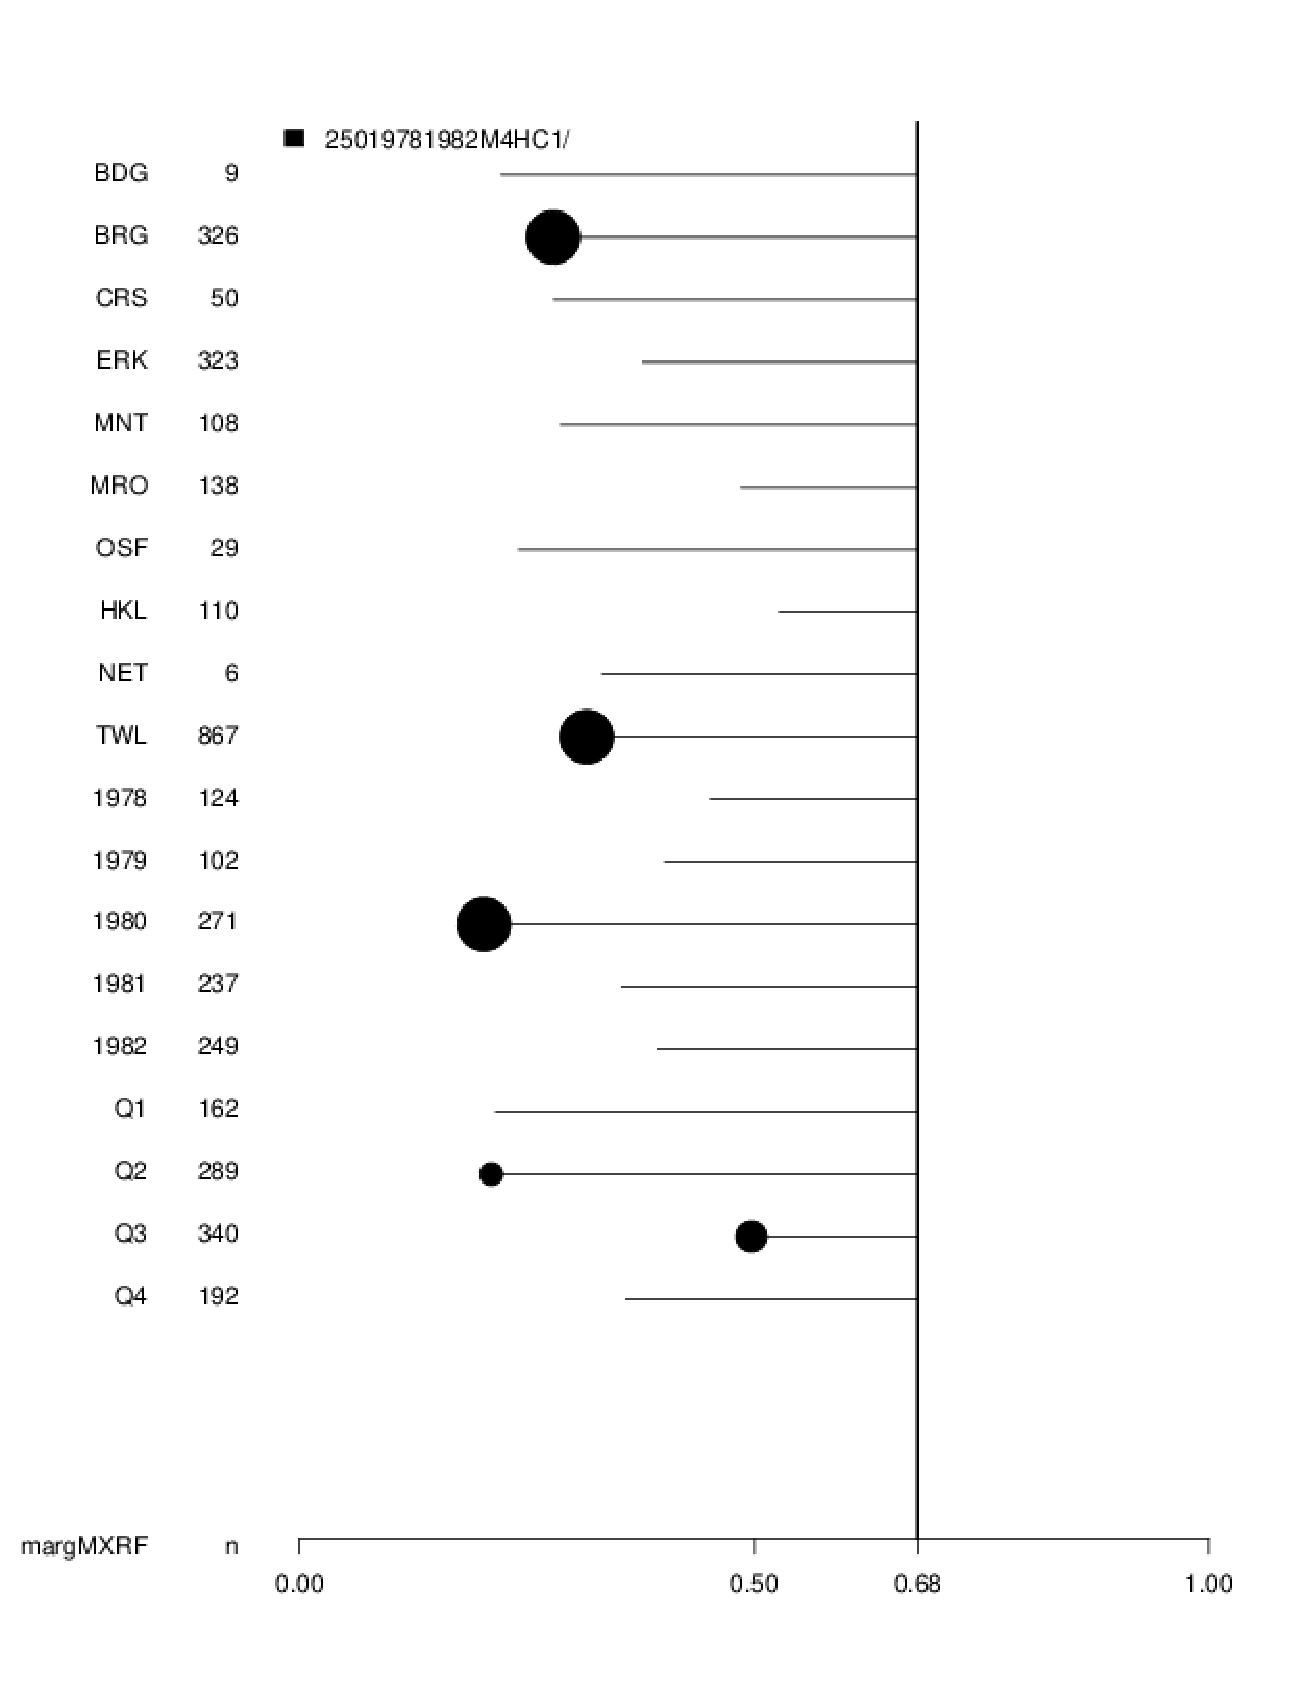
\includegraphics[height=1.1\textheight]{{./postSSC/25019781982M2M3M4/margMXRF/margMXRF-0.68-Diagnostic}.pdf}
        %\end{minipage}
        \end{figure}
\end{frame}

%
%

\subsection{MCAT 253}

\begin{frame}{}
	\begin{table}[ht!]
        \centering
        \begin{tabular}[c]{@{}lcccccc@{}}
        \hline
        & \href{https://github.com/gasduster99/sppComp/tree/master/sscRuns/25319781982M1}{M1} & \href{https://github.com/gasduster99/sppComp/tree/master/sscRuns/25319781982M2}{M2} & \href{https://github.com/gasduster99/sppComp/tree/master/sscRuns/25319781982M3}{M3} & \href{https://github.com/gasduster99/sppComp/tree/master/sscRuns/25319781982M4}{M4} & \href{https://github.com/gasduster99/sppComp/tree/master/sscRuns/25319781982M5}{M5} & \href{https://github.com/gasduster99/sppComp/tree/master/sscRuns/25319781982M6}{M6} \\ \hline
	\(\Delta\) DIC & 1409.81 & 0.09 & 0.1 & 0.07 & 0.05 & 0 \\                        
	\(\Delta\) WAIC & 1391.66 & 0.16 & 0.18 & 0 & 0.13 & 0.08 \\ \hline
	%\(pr(M|y)\) & 0 & 0 & 0 & 1 & 0 & 0 \\ \hline
        \end{tabular}
        \end{table}
\end{frame}

%
%

\begin{frame}{$~~~~~~~~~~$ \href{https://github.com/gasduster99/sppComp/tree/master/sscRuns/25319781982M4}{M4} $~~~~~~~~~~~~~~~~~~~~$ \href{https://github.com/gasduster99/sppComp/tree/master/sscRuns/25319781982M5}{M5} $~~~~~~~~~~~~~~~~~~~~$ \href{https://github.com/gasduster99/sppComp/tree/master/sscRuns/25319781982M6}{M6} }	
	\begin{figure}[ht!]
        \centering
	\hspace*{-1cm}
        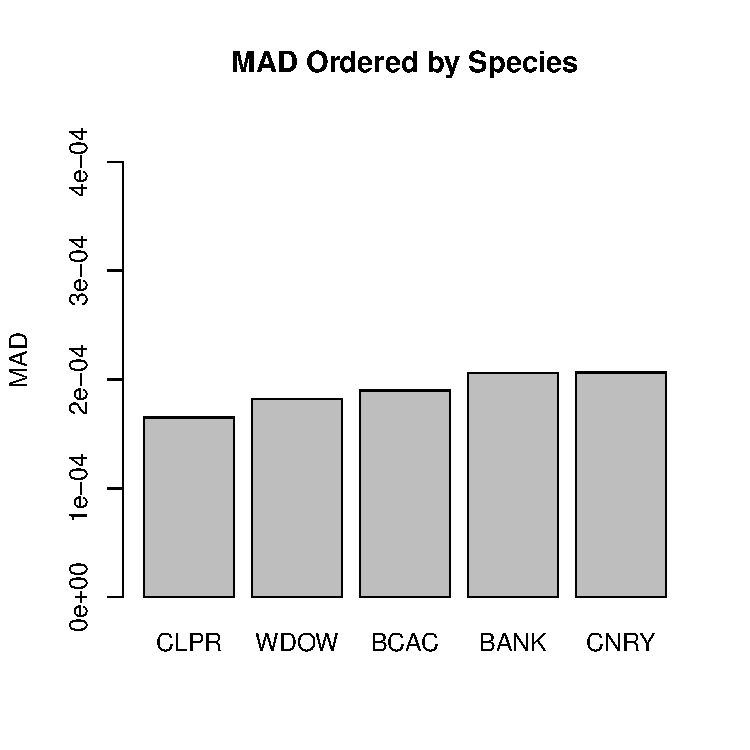
\includegraphics[width=.4\textwidth]{../sscRuns/25319781982M4/sppHeadMad68.pdf}
        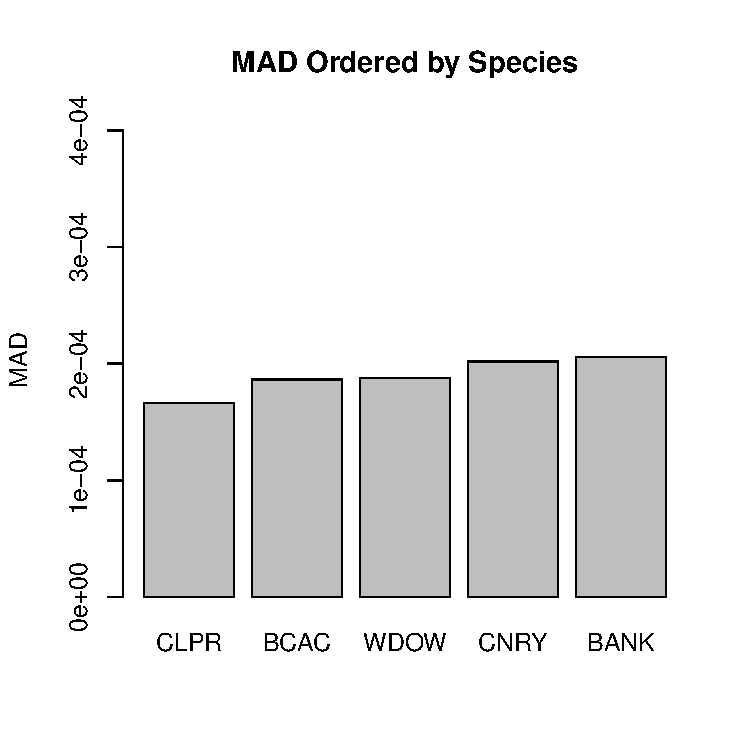
\includegraphics[width=.4\textwidth]{../sscRuns/25319781982M5/sppHeadMad68.pdf}
	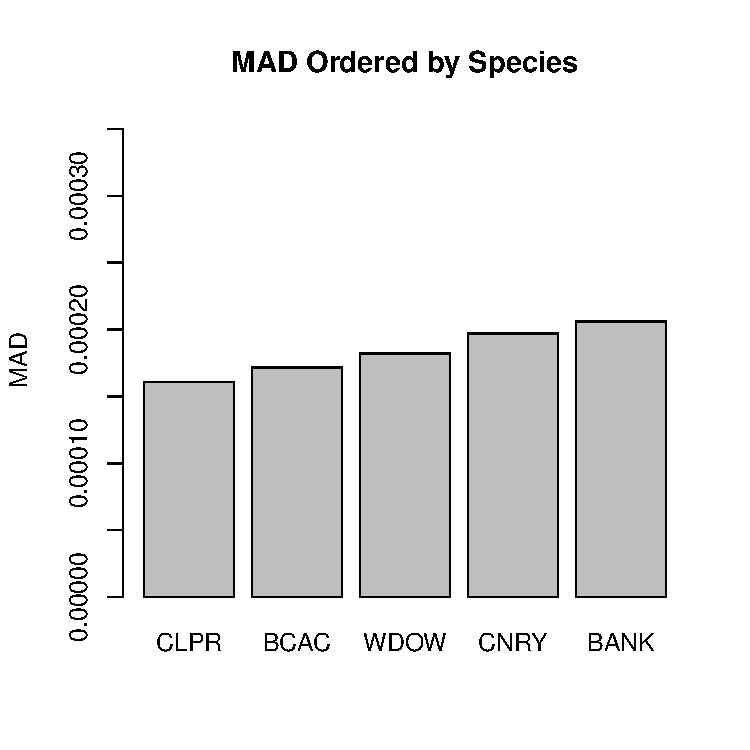
\includegraphics[width=.4\textwidth]{../sscRuns/25319781982M6/sppHeadMad68.pdf}
	\end{figure}
	\vspace{-1cm}
	\begin{center}
	\Large
	\href{https://github.com/gasduster99/sppComp/tree/master/try1/postSSC/25319781982M4M5M6}{Combined}
	\end{center}
\end{frame}

%
%

%
\begin{frame}
        \begin{figure}[ht!]
        \centering
        \vspace{-0.75cm}
        \includegraphics[height=1.1\textheight]{{./postSSC/25319781982M4M5M6/margBCAC/margBCAC-0.68-Diagnostic}.pdf}
        \end{figure}	
\end{frame}

%
%

%
\begin{frame}
	\begin{figure}[ht!]
        \centering
	\vspace{-0.75cm}
	\includegraphics[height=1.1\textheight]{{./postSSC/25319781982M4M5M6/margWDOW/margWDOW-0.68-Diagnostic}.pdf}
	\end{figure}
\end{frame}

%
%

\begin{frame}{$~~~~~~~~~~$ \href{https://github.com/gasduster99/sppComp/tree/master/sscRuns/25319781982M4}{M4} $~~~~~~~~~~~~~~~~~~~~$ \href{https://github.com/gasduster99/sppComp/tree/master/sscRuns/25319781982M5}{M5} $~~~~~~~~~~~~~~~~~~~~$ \href{https://github.com/gasduster99/sppComp/tree/master/sscRuns/25319781982M6}{M6} }	
	\begin{figure}[ht!]
        \centering
	\hspace*{-1cm}
        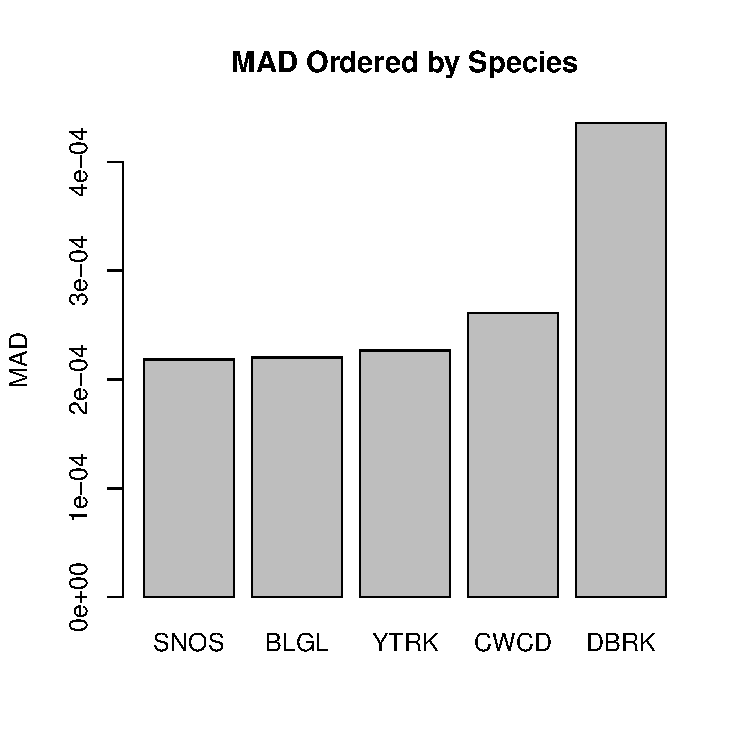
\includegraphics[width=.4\textwidth]{../sscRuns/25319781982M4/sppTailMad68.pdf}
        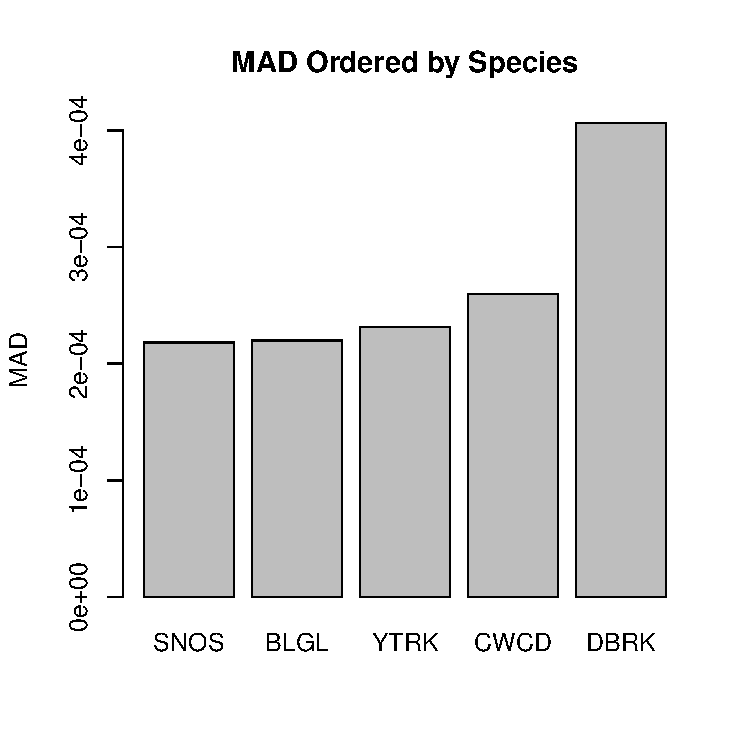
\includegraphics[width=.4\textwidth]{../sscRuns/25319781982M5/sppTailMad68.pdf}
	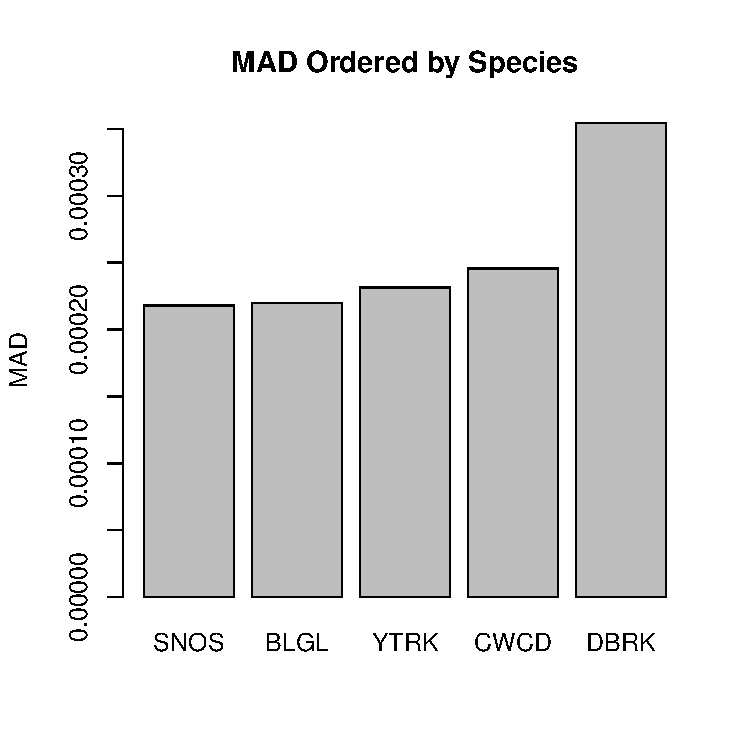
\includegraphics[width=.4\textwidth]{../sscRuns/25319781982M6/sppTailMad68.pdf}
	\end{figure}
	\vspace{-1cm}
	\begin{center}
	\Large
	\href{https://github.com/gasduster99/sppComp/tree/master/try1/postSSC/25319781982M4M5M6}{Combined}
	\end{center}
\end{frame}

%
%

%
\begin{frame}
        \begin{figure}[ht!]
        \centering
        \vspace{-0.75cm}
        \includegraphics[height=1.1\textheight]{{./postSSC/25319781982M4M5M6/margCWCD/margCWCD-0.68-Diagnostic}.pdf}
        \end{figure}    
\end{frame}

%
%

%
\begin{frame}
        \begin{figure}[ht!]
        \centering
        \vspace{-0.75cm}
        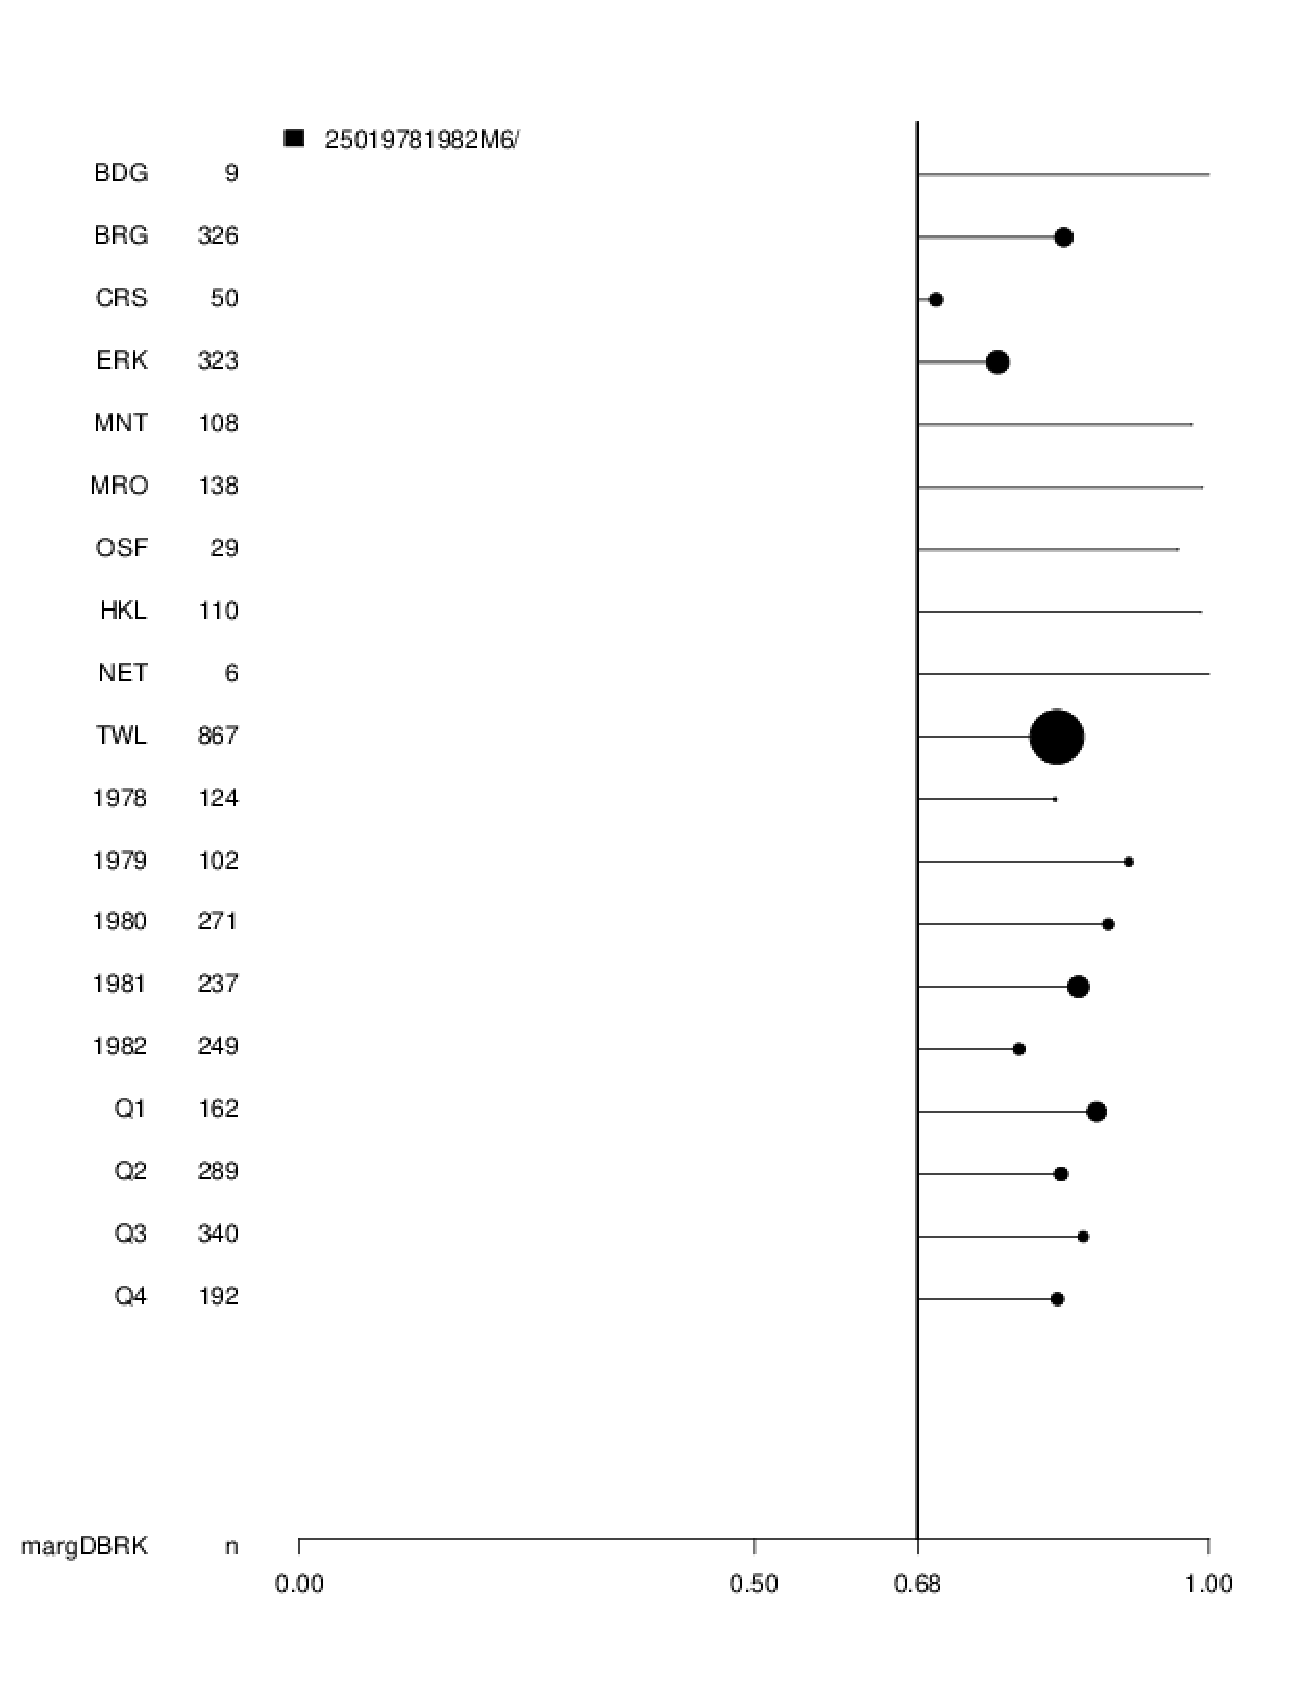
\includegraphics[height=1.1\textheight]{{./postSSC/25319781982M4M5M6/margDBRK/margDBRK-0.68-Diagnostic}.pdf}
        \end{figure}
\end{frame}

%
%

\subsection{MCAT 269}
\begin{frame}{}
	\begin{table}[ht!]
        \centering
        \begin{tabular}[c]{@{}lcccccc@{}}
        \hline
        & \href{https://github.com/gasduster99/sppComp/tree/master/sscRuns/26919781982M1}{M1} & \href{https://github.com/gasduster99/sppComp/tree/master/sscRuns/26919781982M2}{M2} & \href{https://github.com/gasduster99/sppComp/tree/master/sscRuns/26919781982M3}{M3} & \href{https://github.com/gasduster99/sppComp/tree/master/sscRuns/26919781982M4}{M4} & \href{https://github.com/gasduster99/sppComp/tree/master/sscRuns/26919781982M5}{M5} & \href{https://github.com/gasduster99/sppComp/tree/master/sscRuns/26919781982M6}{M6} \\ \hline
	\(\Delta\) DIC & 572.51 & 176.63 & 599.41 & 0.57 & 0 & 193.35 \\
	\(\Delta\) WAIC & 427.48 & 69.37 & 454.41 & 0.23 & 0 & 78.07 \\ \hline
	%\(pr(M|y)\) & 0 & 0 & 0 & 0 & 0 & 1 \\ \hline
        \end{tabular}
        \end{table}
\end{frame}

%
%

\begin{frame}{$~~~~~~~~~~$ \href{https://github.com/gasduster99/sppComp/tree/master/sscRuns/26919781982M4}{M4} $~~~~~~~~~~~~~~~~~~~~$ \href{https://github.com/gasduster99/sppComp/tree/master/sscRuns/26919781982M5}{M5} $~~~~~~~~~~~~~~~~~~~~$ \href{https://github.com/gasduster99/sppComp/tree/master/sscRuns/26919781982M6}{M6} }	
	\begin{figure}[ht!]
        \centering
	\hspace*{-1cm}
        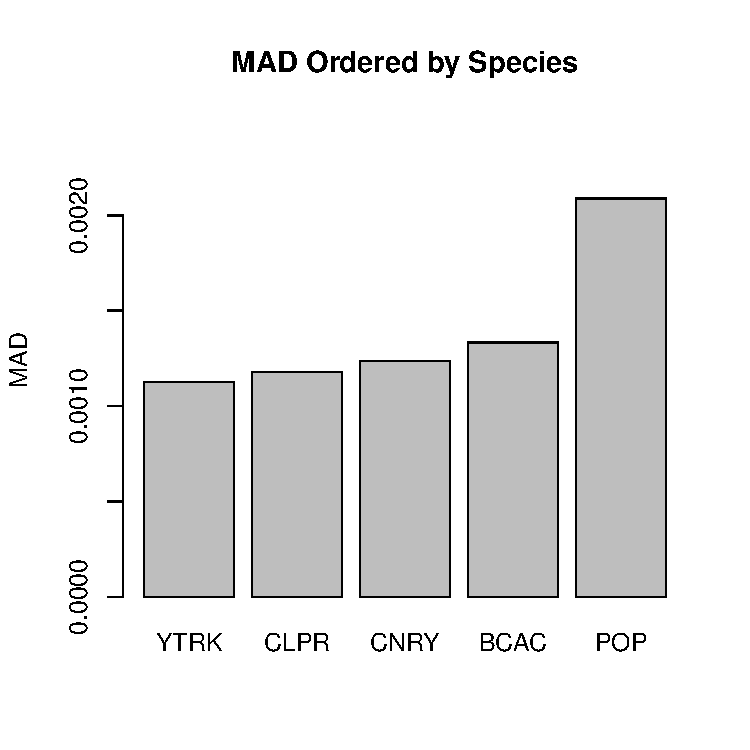
\includegraphics[width=.4\textwidth]{../sscRuns/26919781982M4/sppHeadMad68.pdf}
        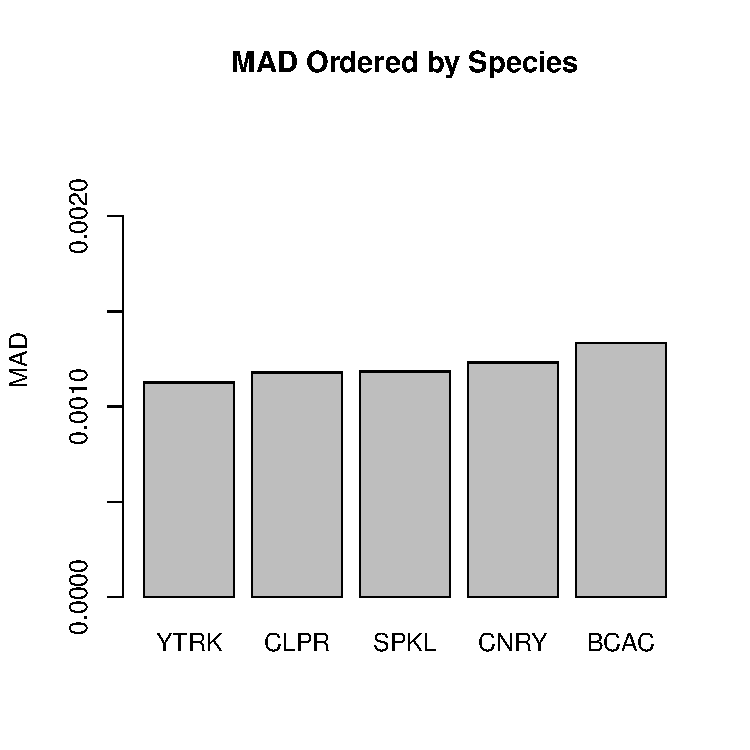
\includegraphics[width=.4\textwidth]{../sscRuns/26919781982M5/sppHeadMad68.pdf}
	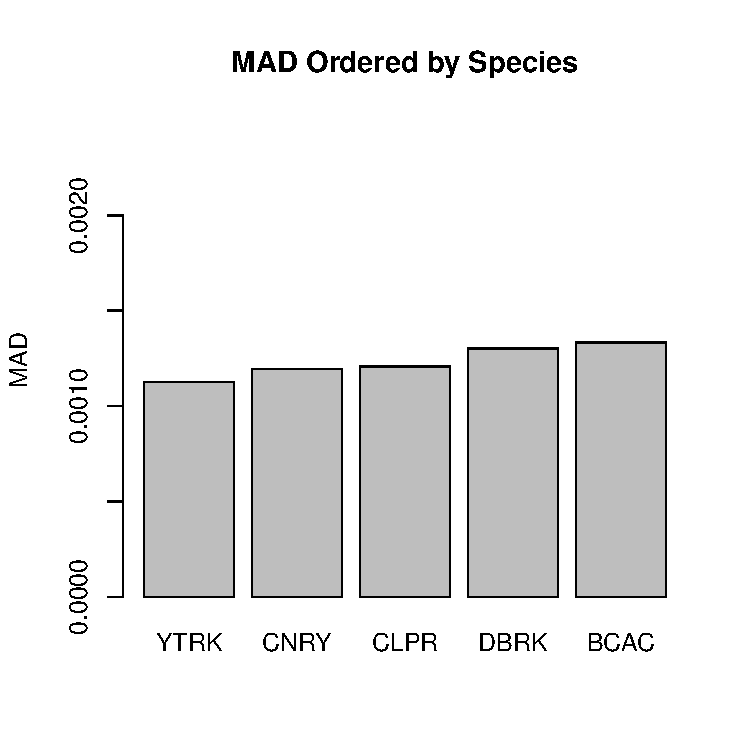
\includegraphics[width=.4\textwidth]{../sscRuns/26919781982M6/sppHeadMad68.pdf}
	\end{figure}
	\vspace{-1cm}
	\begin{center}
	\Large
	\href{https://github.com/gasduster99/sppComp/tree/master/try1/postSSC/26919781982M4M5M6}{Combined}
	\end{center}
\end{frame}

%
%

%
\begin{frame}
        \begin{figure}[ht!]
        \centering
        \vspace{-0.75cm}
        \includegraphics[height=1.1\textheight]{{./postSSC/26919781982M4M5M6/margCNRY/margCNRY-0.68-Diagnostic}.pdf}
        \end{figure}	
\end{frame}

%
%

%
\begin{frame}
        \begin{figure}[ht!]
        \centering
        \vspace{-0.75cm}
        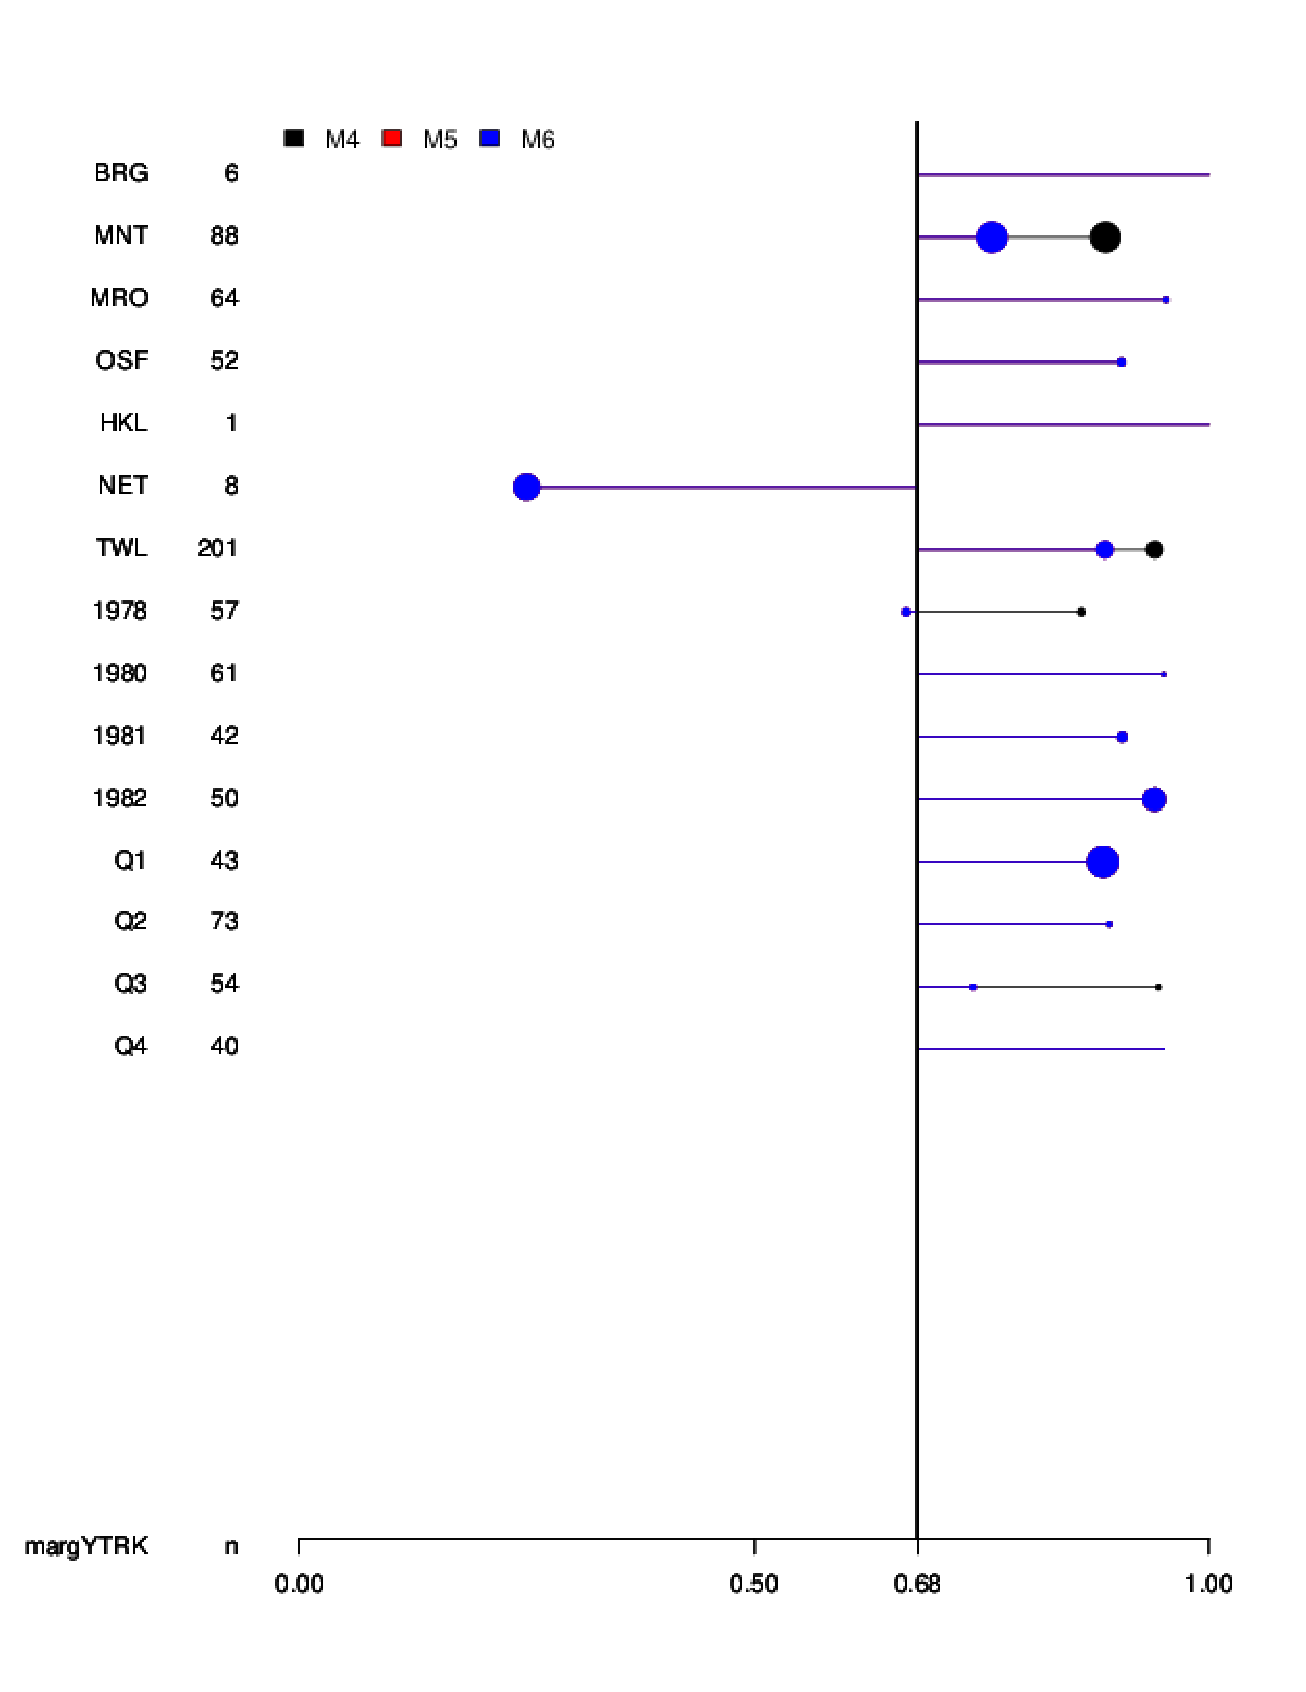
\includegraphics[height=1.1\textheight]{{./postSSC/26919781982M4M5M6/margYTRK/margYTRK-0.68-Diagnostic}.pdf}
        \end{figure}	
\end{frame}

%
%

\begin{frame}{$~~~~~~~~~~$ \href{https://github.com/gasduster99/sppComp/tree/master/sscRuns/26919781982M4}{M4} $~~~~~~~~~~~~~~~~~~~~$ \href{https://github.com/gasduster99/sppComp/tree/master/sscRuns/26919781982M5}{M5} $~~~~~~~~~~~~~~~~~~~~$ \href{https://github.com/gasduster99/sppComp/tree/master/sscRuns/26919781982M6}{M6} }	
	\begin{figure}[ht!]
        \centering
	\hspace*{-1cm}
        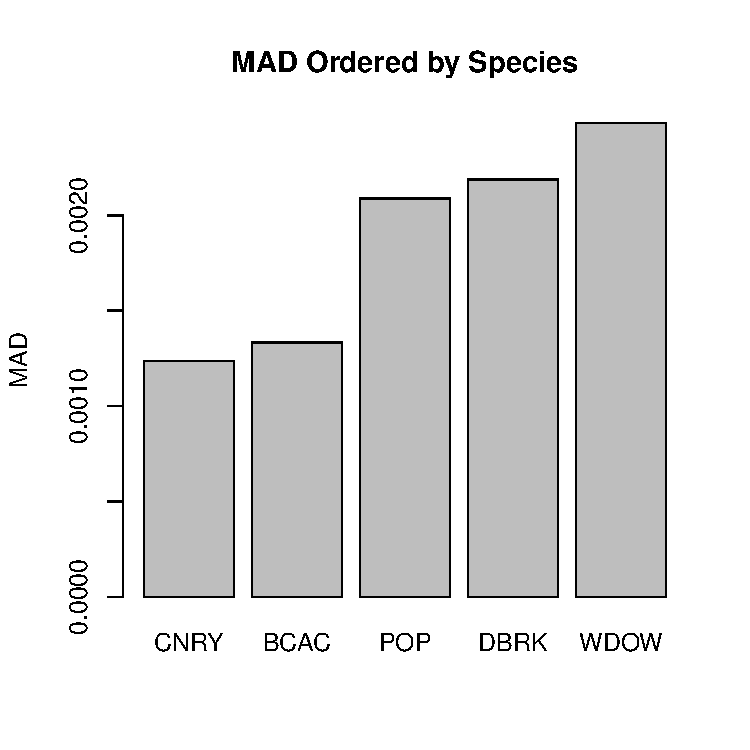
\includegraphics[width=.4\textwidth]{../sscRuns/26919781982M4/sppTailMad68.pdf}
        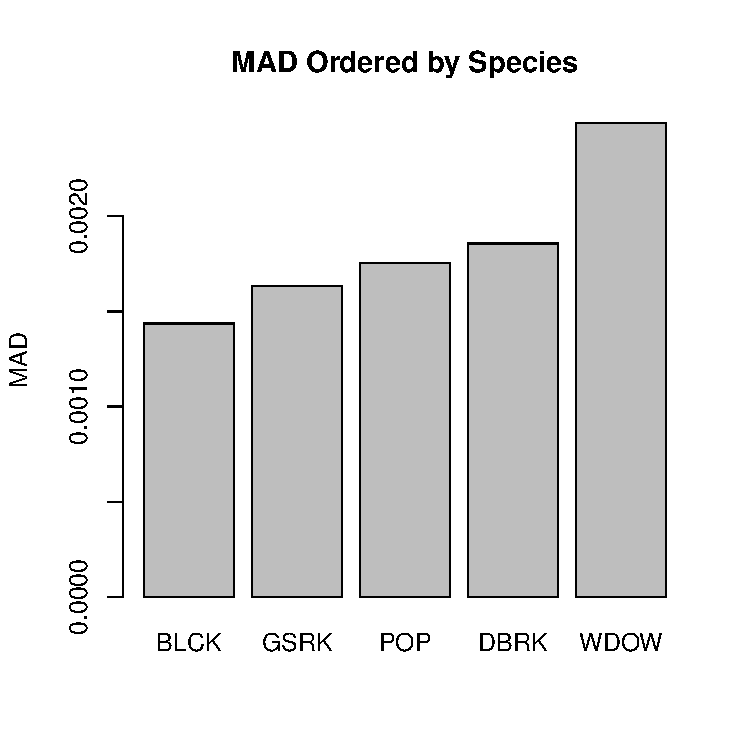
\includegraphics[width=.4\textwidth]{../sscRuns/26919781982M5/sppTailMad68.pdf}
	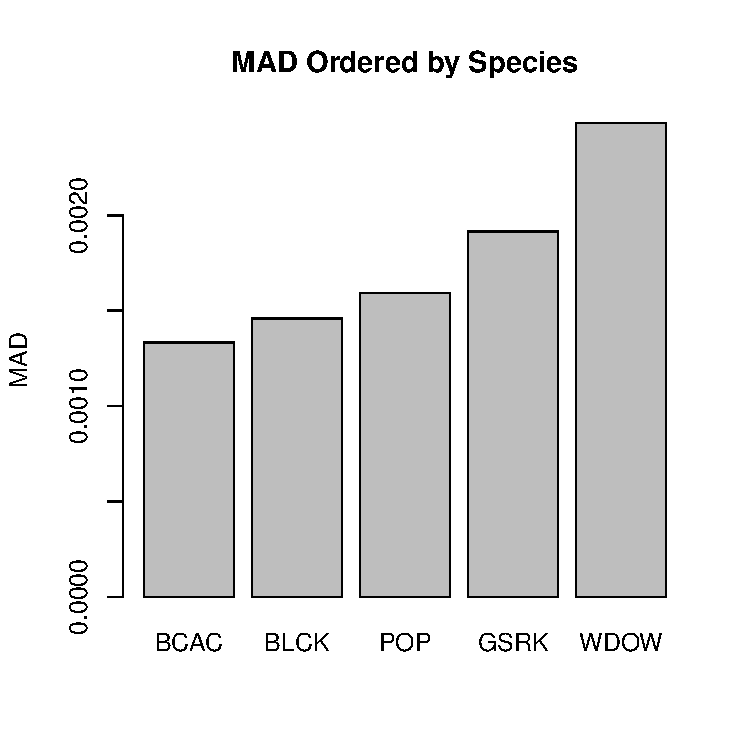
\includegraphics[width=.4\textwidth]{../sscRuns/26919781982M6/sppTailMad68.pdf}
	\end{figure}
	\vspace{-1cm}
	\begin{center}
	\Large
	\href{https://github.com/gasduster99/sppComp/tree/master/try1/postSSC/26919781982M4M5M6}{Combined}
	\end{center}
\end{frame}

%
%

%
\begin{frame}
        \begin{figure}[ht!]
        \centering
        \vspace{-0.75cm}
        \includegraphics[height=1.1\textheight]{{./postSSC/26919781982M4M5M6/margBCAC/margBCAC-0.68-Diagnostic}.pdf}
        \end{figure}    
\end{frame}

%
%

%
\begin{frame}
        \begin{figure}[ht!]
        \centering
        \vspace{-0.75cm}
        \includegraphics[height=1.1\textheight]{{./postSSC/26919781982M4M5M6/margWDOW/margWDOW-0.68-Diagnostic}.pdf}
        \end{figure}
\end{frame}

%
%

%
\subsection{Landings Sensitivity}
%\subsection{}
\begin{frame}
\textbf{Request:}
Compare alternative ComX outputs and the current time series of estimated 
catches.

\textbf{Rationale:}  
It would be informative to see the landings estimates corresponding to the 
additional models developed in response to the above requests.  The landings 
estimates can be generated for a small set of illustrative species and do not 
need to be comprehensive.

\textbf{Response:}
The following slides show expanded landings (by year and by year:gear) from 
the early time period, summing across market categories 250, 253, and 269 
associated with time model, prior, interaction model, and time block 
sensitivity runs.

\end{frame}

%
%

%
\begin{frame}	
	\vspace{-0.15cm}
	\begin{minipage}{0.49\textwidth}
		\centering
		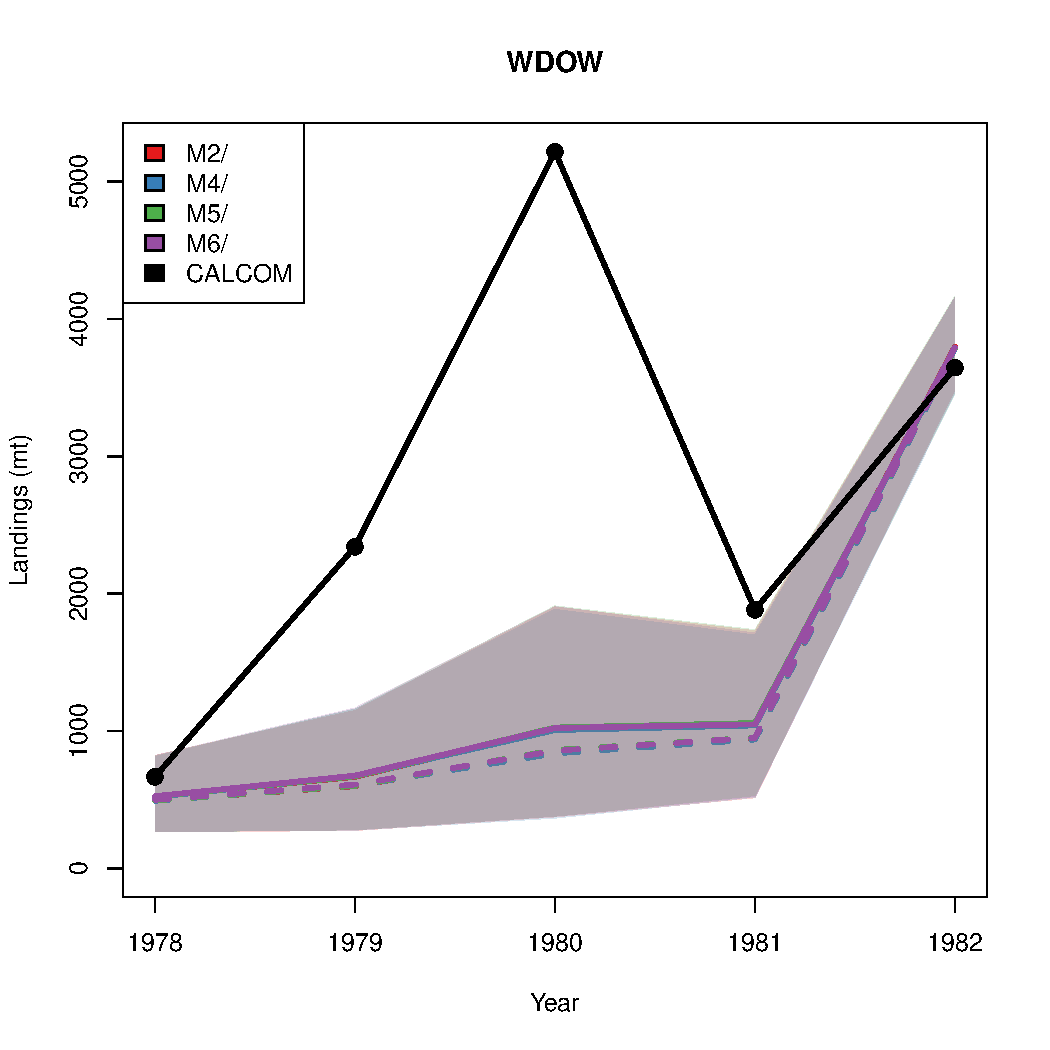
\includegraphics[height=0.54\textheight]{./postSSC/landDiagnostics/M2M3M4M5M6/WDOW/yearWDOW.pdf}
		\\\vspace{-0.25cm}
		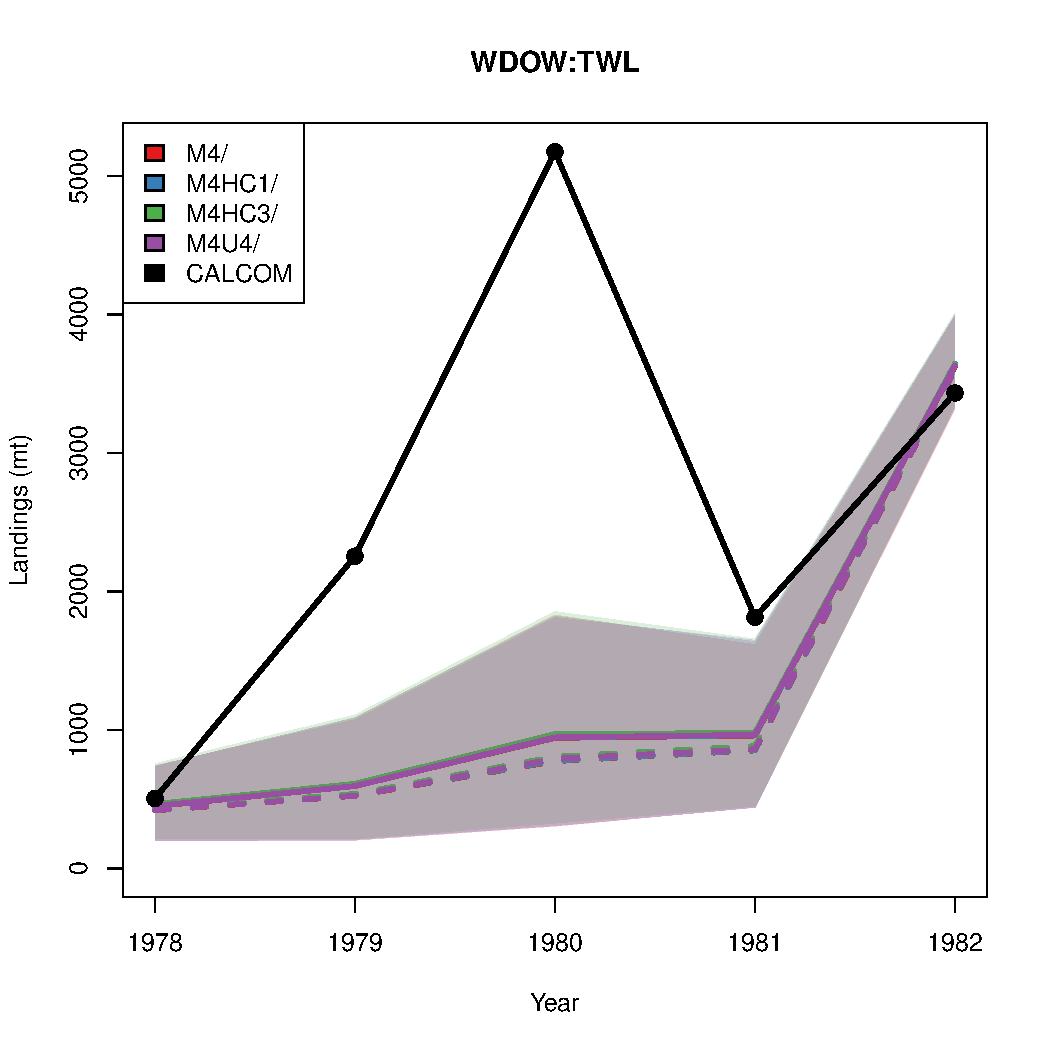
\includegraphics[height=0.54\textheight]{{./postSSC/landDiagnostics/M2M3M4M5M6/WDOW/yearGearWDOW-TWL}.pdf}
	\end{minipage}
	\begin{minipage}{0.49\textwidth}
		\centering	
		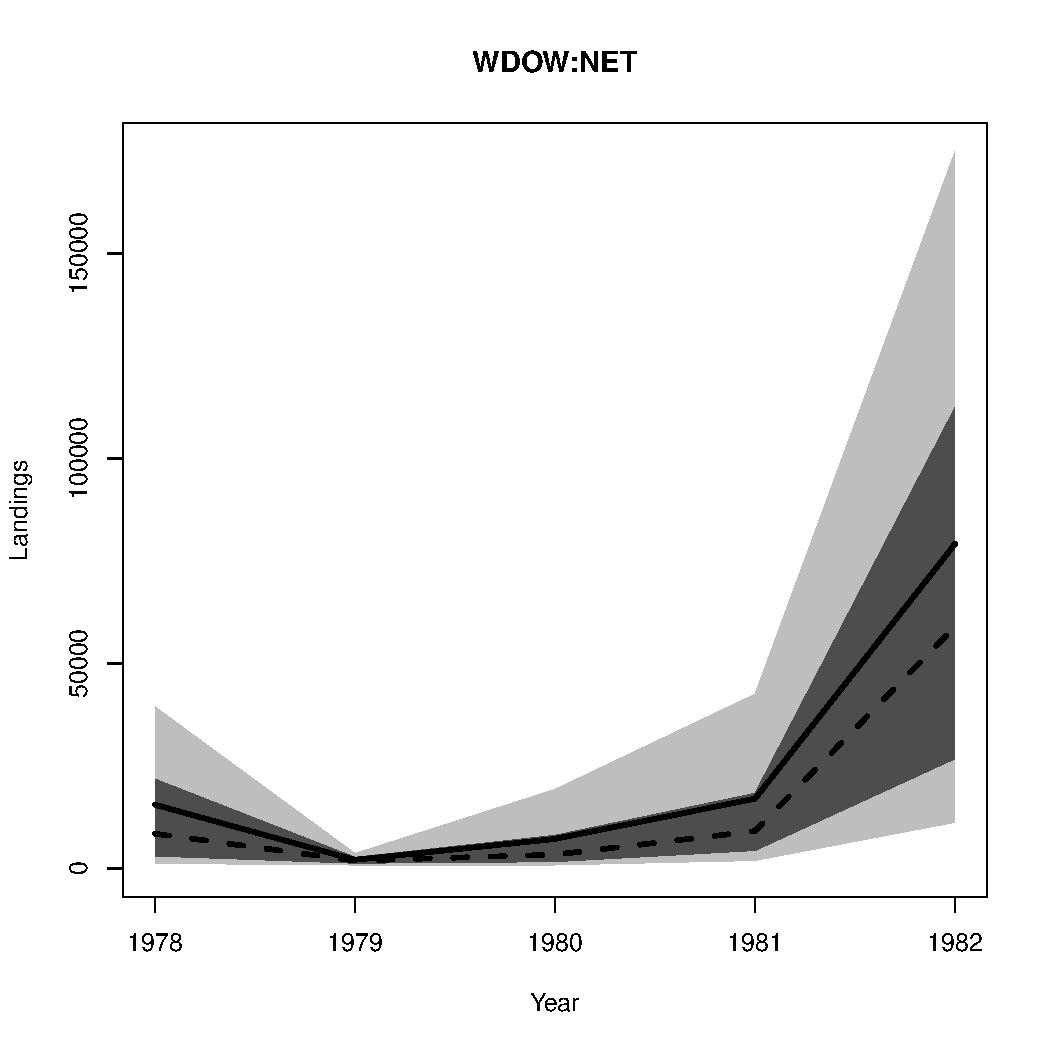
\includegraphics[height=0.54\textheight]{{./postSSC/landDiagnostics/M2M3M4M5M6/WDOW/yearGearWDOW-NET}.pdf}
		\\\vspace{-0.25cm}
		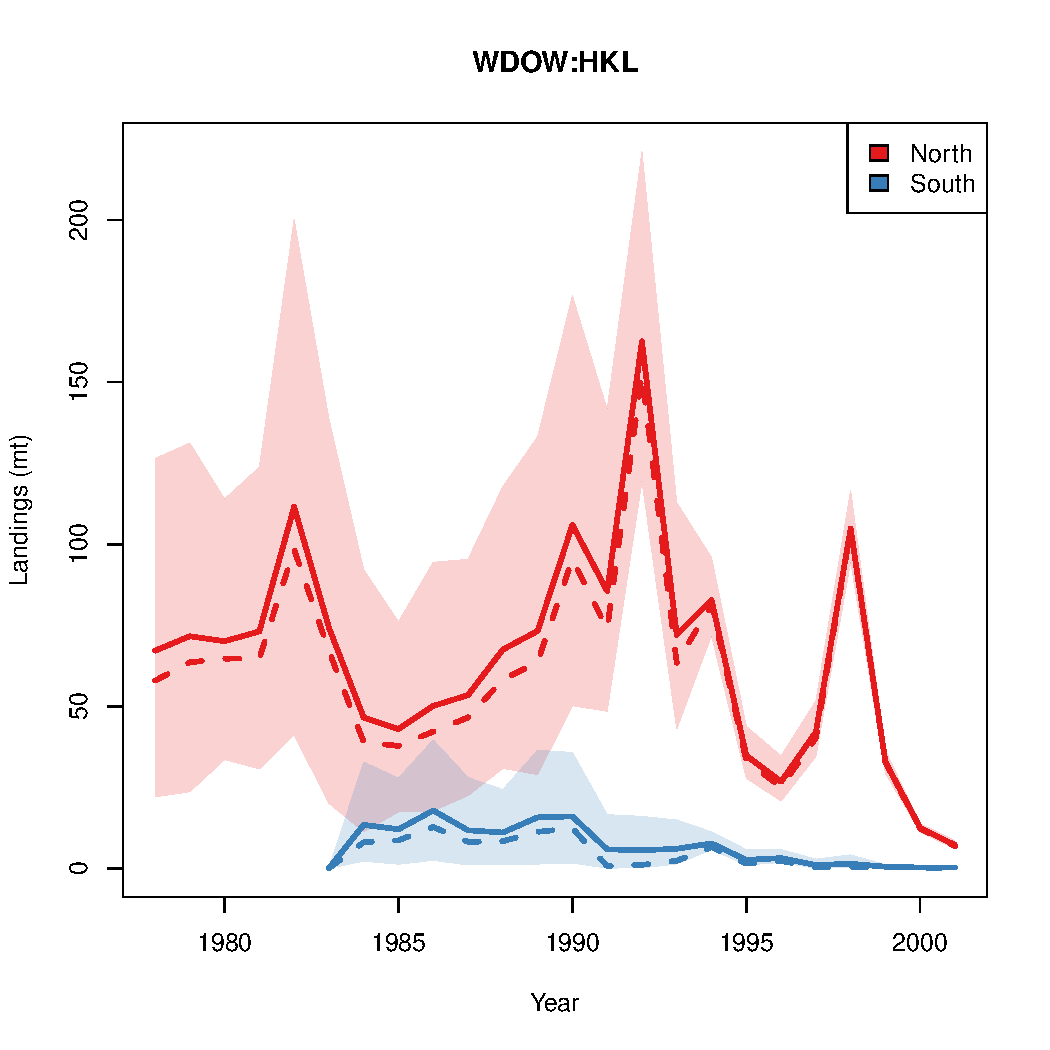
\includegraphics[height=0.54\textheight]{{./postSSC/landDiagnostics/M2M3M4M5M6/WDOW/yearGearWDOW-HKL}.pdf}
	\end{minipage}
\end{frame}

%
%

%
\begin{frame}	
	\vspace{-0.15cm}
	\begin{minipage}{0.49\textwidth}
		\centering
		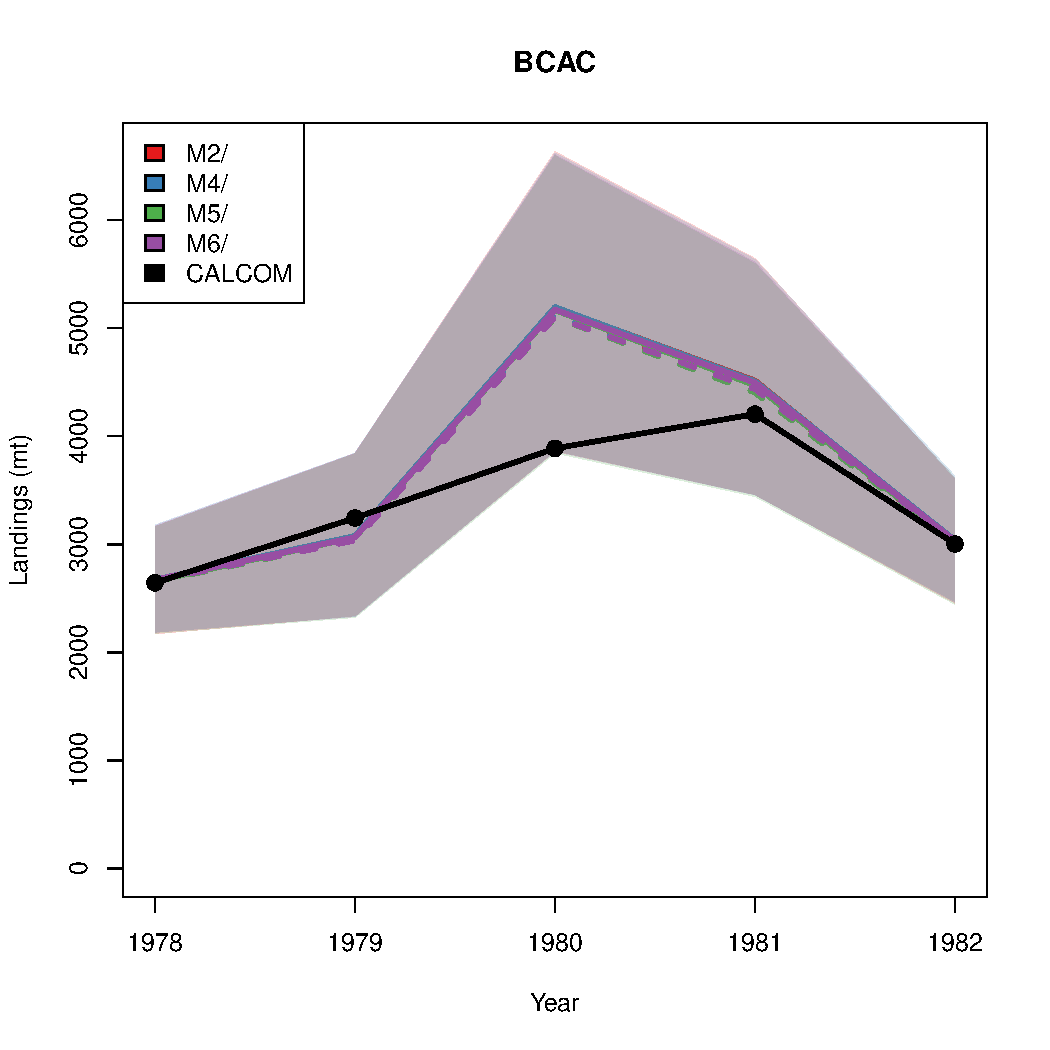
\includegraphics[height=0.54\textheight]{./postSSC/landDiagnostics/M2M3M4M5M6/BCAC/yearBCAC.pdf}
		\\\vspace{-0.25cm}
		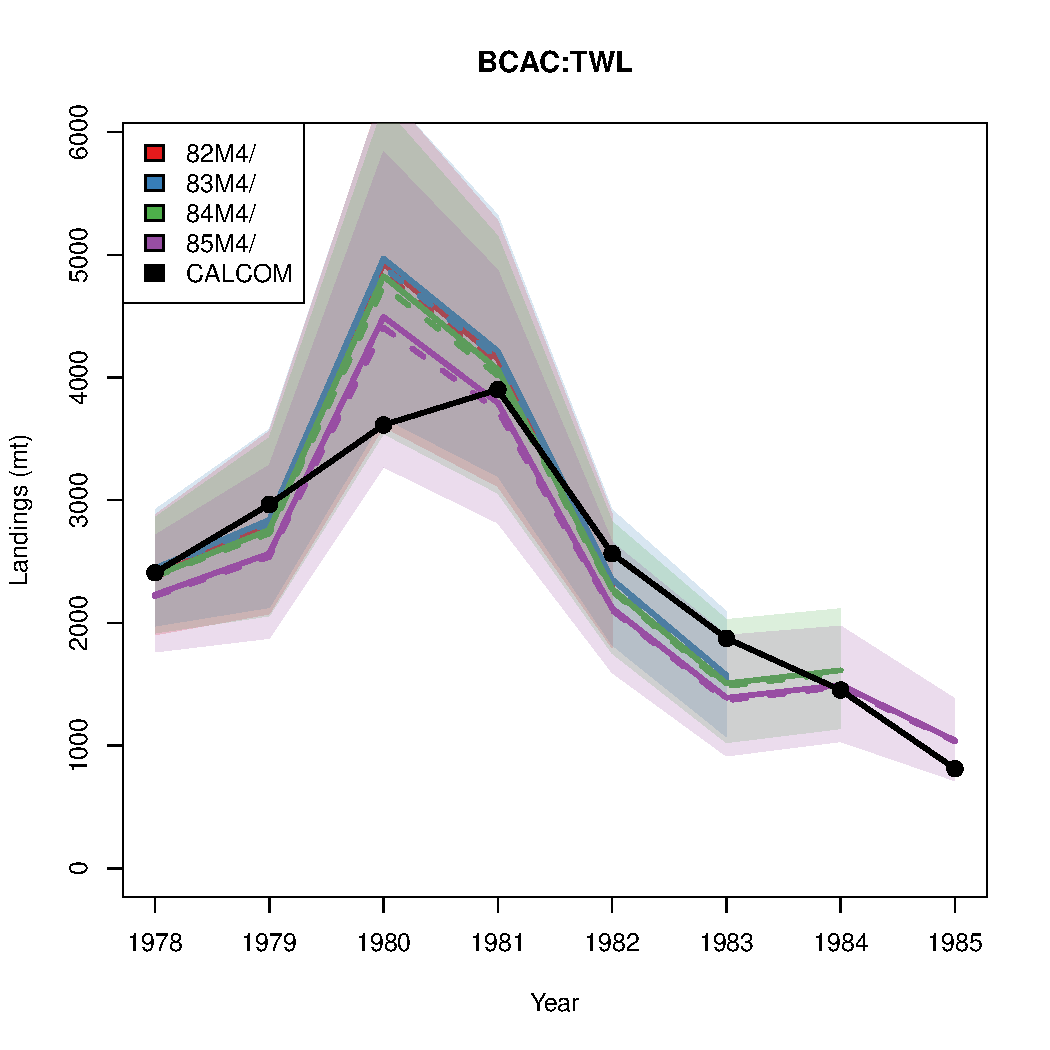
\includegraphics[height=0.54\textheight]{{./postSSC/landDiagnostics/M2M3M4M5M6/BCAC/yearGearBCAC-TWL}.pdf}
	\end{minipage}
	\begin{minipage}{0.49\textwidth}
		\centering	
		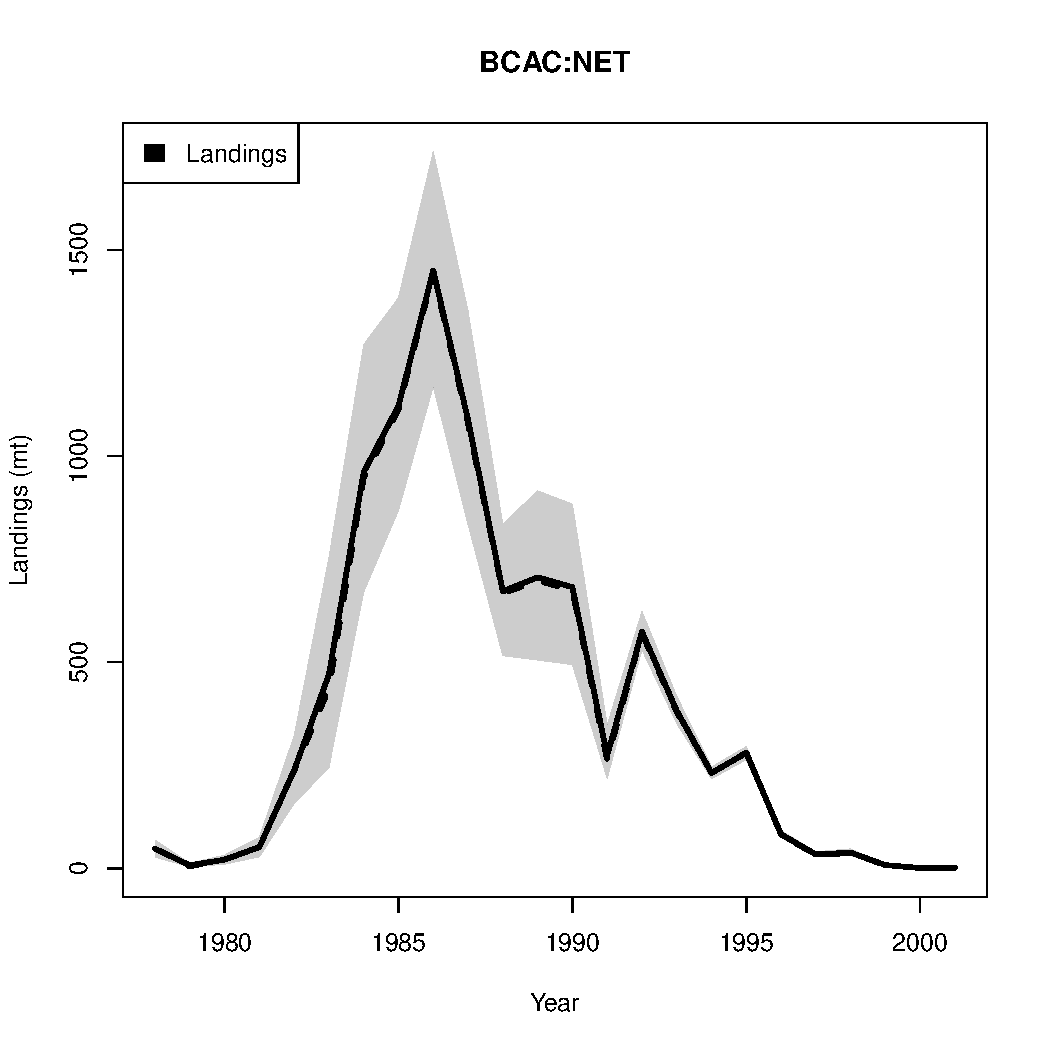
\includegraphics[height=0.54\textheight]{{./postSSC/landDiagnostics/M2M3M4M5M6/BCAC/yearGearBCAC-NET}.pdf}
		\\\vspace{-0.25cm}
		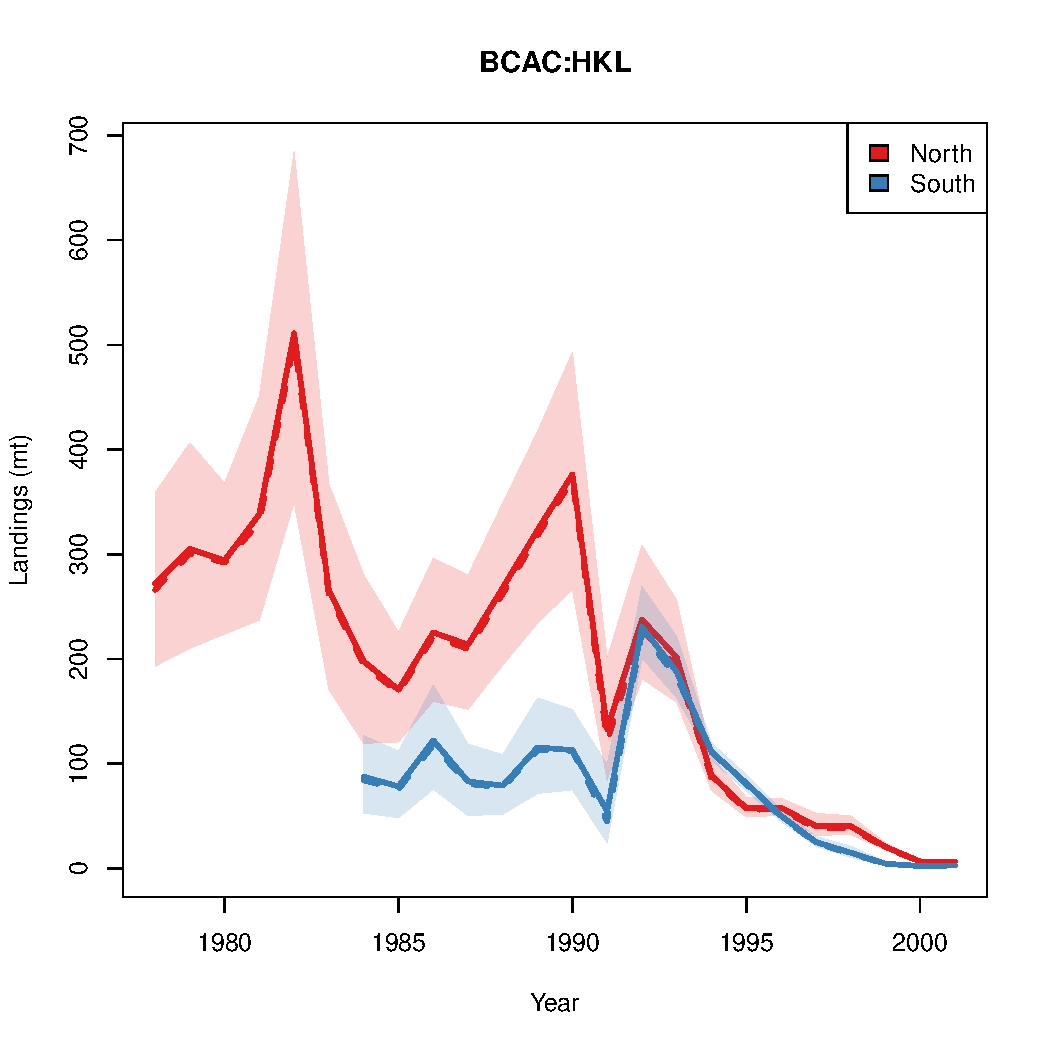
\includegraphics[height=0.54\textheight]{{./postSSC/landDiagnostics/M2M3M4M5M6/BCAC/yearGearBCAC-HKL}.pdf}
	\end{minipage}
\end{frame}

%
%

%
\begin{frame}	
	\vspace{-0.15cm}
	\begin{minipage}{0.49\textwidth}
		\centering
		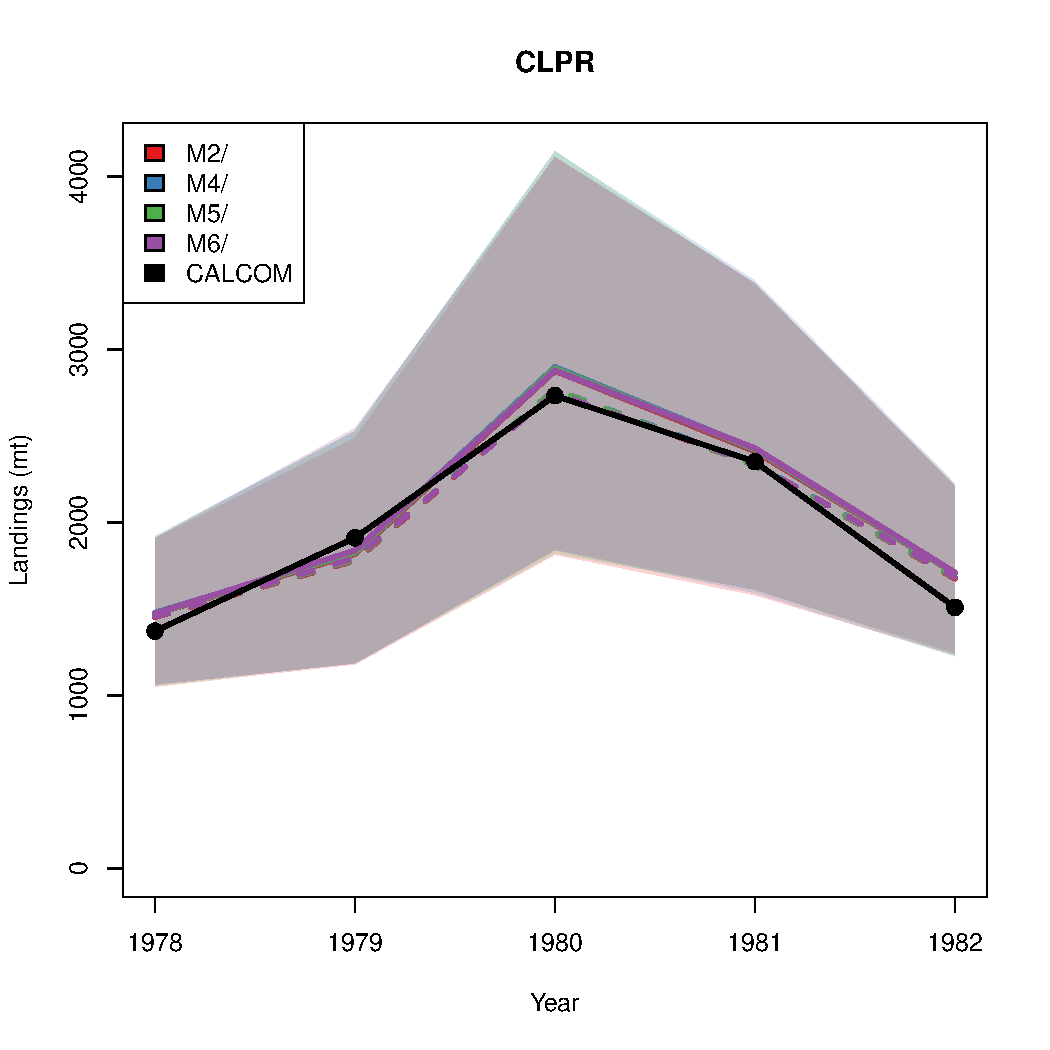
\includegraphics[height=0.54\textheight]{./postSSC/landDiagnostics/M2M3M4M5M6/CLPR/yearCLPR.pdf}
		\\\vspace{-0.25cm}
		\includegraphics[height=0.54\textheight]{{./postSSC/landDiagnostics/M2M3M4M5M6/CLPR/yearGearCLPR-TWL}.pdf}
	\end{minipage}
	\begin{minipage}{0.49\textwidth}
		\centering	
		\includegraphics[height=0.54\textheight]{{./postSSC/landDiagnostics/M2M3M4M5M6/CLPR/yearGearCLPR-NET}.pdf}
		\\\vspace{-0.25cm}
		\includegraphics[height=0.54\textheight]{{./postSSC/landDiagnostics/M2M3M4M5M6/CLPR/yearGearCLPR-HKL}.pdf}
	\end{minipage}
\end{frame}

%
%

%
\begin{frame}	
	\vspace{-0.15cm}
	\begin{minipage}{0.49\textwidth}
		\centering
		\includegraphics[height=0.54\textheight]{./postSSC/landDiagnostics/M2M3M4M5M6/DBRK/yearDBRK.pdf}
		\\\vspace{-0.25cm}
		\includegraphics[height=0.54\textheight]{{./postSSC/landDiagnostics/M2M3M4M5M6/DBRK/yearGearDBRK-TWL}.pdf}
	\end{minipage}
	\begin{minipage}{0.49\textwidth}
		\centering	
		\includegraphics[height=0.54\textheight]{{./postSSC/landDiagnostics/M2M3M4M5M6/DBRK/yearGearDBRK-NET}.pdf}
		\\\vspace{-0.25cm}
		\includegraphics[height=0.54\textheight]{{./postSSC/landDiagnostics/M2M3M4M5M6/DBRK/yearGearDBRK-HKL}.pdf}
	\end{minipage}
\end{frame}

%
%

%
\begin{frame}	
	\vspace{-0.15cm}
	\begin{minipage}{0.49\textwidth}
		\centering
		\includegraphics[height=0.54\textheight]{./postSSC/landDiagnostics/M2M3M4M5M6/CWCD/yearCWCD.pdf}
		\\\vspace{-0.25cm}
		\includegraphics[height=0.54\textheight]{{./postSSC/landDiagnostics/M2M3M4M5M6/CWCD/yearGearCWCD-TWL}.pdf}
	\end{minipage}
	\begin{minipage}{0.49\textwidth}
		\centering	
		\includegraphics[height=0.54\textheight]{{./postSSC/landDiagnostics/M2M3M4M5M6/CWCD/yearGearCWCD-NET}.pdf}
		\\\vspace{-0.25cm}
		\includegraphics[height=0.54\textheight]{{./postSSC/landDiagnostics/M2M3M4M5M6/CWCD/yearGearCWCD-HKL}.pdf}
	\end{minipage}
\end{frame}

%
%

%
\begin{frame}	
	\vspace{-0.15cm}
	\begin{minipage}{0.49\textwidth}
		\centering
		\includegraphics[height=0.54\textheight]{./postSSC/landDiagnostics/M2M3M4M5M6/MXRF/yearMXRF.pdf}
		\\\vspace{-0.25cm}
		\includegraphics[height=0.54\textheight]{{./postSSC/landDiagnostics/M2M3M4M5M6/MXRF/yearGearMXRF-TWL}.pdf}
	\end{minipage}
	\begin{minipage}{0.49\textwidth}
		\centering	
		\includegraphics[height=0.54\textheight]{{./postSSC/landDiagnostics/M2M3M4M5M6/MXRF/yearGearMXRF-NET}.pdf}
		\\\vspace{-0.25cm}
		\includegraphics[height=0.54\textheight]{{./postSSC/landDiagnostics/M2M3M4M5M6/MXRF/yearGearMXRF-HKL}.pdf}
	\end{minipage}
\end{frame}

%
%

%
\begin{frame}{Time Model Summary}	
        \begin{minipage}{0.49\textwidth}
	\begin{itemize}
	\item The time model appears to be slightly dependent on market category, although several models perform similarly. 
	\item M4 generally performs well in a data-poor environment.
	\item Differences are small in a data-rich environment.
	\end{itemize}
	\end{minipage}
        \begin{minipage}{0.49\textwidth}
	\begin{center}
	\href{https://github.com/gasduster99/sppComp/tree/master/try1/postSSC/25019781982M2M3M4}{MCAT 250 Combined Plots}\\$~$\\
	\href{https://github.com/gasduster99/sppComp/tree/master/try1/postSSC/25319781982M4M5M6}{MCAT 253 Combined Plots}\\$~$\\
	\href{https://github.com/gasduster99/sppComp/tree/master/try1/postSSC/26919781982M4M5M6}{MCAT 269 Combined Plots}\\$~$\\
	\href{https://github.com/gasduster99/sppComp/tree/master/try1/postSSC/landDiagnostics/M2M3M4M5M6}{All Species Landings}
	\end{center}
	\end{minipage}
\end{frame}



%
%

%
\section{Prior Model}
\subsection{}
\begin{frame}{Priors}
$~$
\hspace*{-1.5cm}
\begin{minipage}{0.45\textwidth}
%\vspace{-0.5cm}
\begin{align*}
&\\
\beta_0 &\propto 1\\
\beta^{(s)}_j &\sim N(0, 32^2)\\
\beta^{(p)}_k &\sim N(0, 32^2)\\
\beta^{(g)}_l &\sim N(0, 32^2)\\
\text{logit}(\rho) &\sim N(0, 2^2)\\
\end{align*}
\end{minipage}
\begin{minipage}{0.55\textwidth}
\begin{align*}
\text{IG}  &: ~~v \sim \text{Inv-Gamma}(1,~2x10^{3}) ~~~\forall~~~v \\ 
\text{HC1} &: \sqrt{v} \sim \text{Half-Cauchy}(10^1) \hspace{0.05cm}~~~~~~~~\forall~~~v \\
\text{HC3} &: \sqrt{v} \sim \text{Half-Cauchy}(10^3) \hspace{0.05cm}~~~~~~~~\forall~~~v \\
\text{U4}  &: \sqrt{v} \sim \text{Uniform}(0, 10^4) ~~~~~~~~~~~\forall~~~v
%v\sim IG(1,~&2x10^{3}) ~~~\forall~~~v 
%v\sim IG(1,~&2x10^{3}) ~~~\forall~~~v 
%v\sim IG(1,~&2x10^{3}) ~~~\forall~~~v 
%&\sqrt{v} \sim \text{Half-Cauchy}(\gamma)&\\ %10)&\\
%&\sqrt{v} \sim \text{Unif}(0, 10^4)&
\end{align*}
\end{minipage}
\end{frame}

%
%

\subsection{MCAT 250}
\begin{frame}{}
        \begin{table}[ht!]
        \centering
        \begin{tabular}[c]{@{}lcccccc@{}}
        %\toprule
        \hline
        & \href{https://github.com/gasduster99/sppComp/tree/master/sscRuns/25019781982M4}{M4IG} & \href{https://github.com/gasduster99/sppComp/tree/master/sscRuns/25019781982M4HC1}{M4HC1} & \href{https://github.com/gasduster99/sppComp/tree/master/sscRuns/25019781982M4HC3}{M4HC3} & \href{https://github.com/gasduster99/sppComp/tree/master/sscRuns/25019781982M4U4}{M4U4} \\ \hline
        \(\Delta\) DIC & 3.87 & 0.02 & 0.1 & 0 \\                                         
	\(\Delta\) WAIC & 3.78 & 0.03 & 0.11 & 0 \\ \hline                                      
	%\(pr(M|y)\) & 0 & 0.21 & 0.37 & 0.42 \\ \hline
	\end{tabular}
        \end{table}
\end{frame}

%
%

%
\begin{frame}{$~~~~~~~$ \href{https://github.com/gasduster99/sppComp/tree/master/sscRuns/25019781982M4HC1}{M4HC1} $~~~~~~~~~~~~~~$ \href{https://github.com/gasduster99/sppComp/tree/master/sscRuns/25019781982M4HC3}{M4HC3} $~~~~~~~~~~~~~~~~~$ \href{https://github.com/gasduster99/sppComp/tree/master/sscRuns/25019781982M4U4}{M4U4} }
        \begin{figure}[ht!]
        \centering
        \hspace*{-1cm}
        \includegraphics[width=.4\textwidth]{../sscRuns/25019781982M4HC1/sppHeadMad68.pdf}
        \includegraphics[width=.4\textwidth]{../sscRuns/25019781982M4HC3/sppHeadMad68.pdf}
        \includegraphics[width=.4\textwidth]{../sscRuns/25019781982M4U4/sppHeadMad68.pdf}
        \end{figure}
	\vspace{-1cm}
	\begin{center}
	\Large
	\href{https://github.com/gasduster99/sppComp/tree/master/try1/postSSC/25019781982M4HC1HC3U4}{Combined}
	\end{center}
\end{frame}

%
%

%
\begin{frame}
        \begin{figure}[ht!]
        \centering
        \vspace{-0.75cm}
        \includegraphics[height=1.1\textheight]{{./postSSC/25019781982M4HC1HC3U4/margBCAC/margBCAC-0.68-Diagnostic}.pdf}
        \end{figure}   
\end{frame}

%
%

%
\begin{frame}
       \begin{figure}[ht!]
       \centering
       \vspace{-0.75cm}
       \includegraphics[height=1.1\textheight]{{./postSSC/25019781982M4HC1HC3U4/margWDOW/margWDOW-0.68-Diagnostic}.pdf}
       \end{figure}
\end{frame}

%
%

%
\begin{frame}{$~~~~~~~$ \href{https://github.com/gasduster99/sppComp/tree/master/sscRuns/25019781982M4HC1}{M4HC1} $~~~~~~~~~~~~~~$ \href{https://github.com/gasduster99/sppComp/tree/master/sscRuns/25019781982M4HC3}{M4HC3} $~~~~~~~~~~~~~~~~~$ \href{https://github.com/gasduster99/sppComp/tree/master/sscRuns/25019781982M4U4}{M4U4} }
        \begin{figure}[ht!]
        \centering
        \hspace*{-1cm}
        \includegraphics[width=.4\textwidth]{../sscRuns/25019781982M4HC1/sppTailMad68.pdf}
        \includegraphics[width=.4\textwidth]{../sscRuns/25019781982M4HC3/sppTailMad68.pdf}
        \includegraphics[width=.4\textwidth]{../sscRuns/25019781982M4U4/sppTailMad68.pdf}
        \end{figure}
	\vspace{-1cm}
	\begin{center}
	\Large
	\href{https://github.com/gasduster99/sppComp/tree/master/try1/postSSC/25019781982M4HC1HC3U4}{Combined}
	\end{center}
\end{frame}

%
%

%
\begin{frame}
        \begin{figure}[ht!]
        \centering
        \vspace{-0.75cm}
        \includegraphics[height=1.1\textheight]{{./postSSC/25019781982M4HC1HC3U4/margCWCD/margCWCD-0.68-Diagnostic}.pdf}
        \end{figure}   
\end{frame}

%
%

%
\begin{frame}
       \begin{figure}[ht!]
       \centering
       \vspace{-0.75cm}
       \includegraphics[height=1.1\textheight]{{./postSSC/25019781982M4HC1HC3U4/margMXRF/margMXRF-0.68-Diagnostic}.pdf}
       \end{figure}
\end{frame}

%
%

%
\subsection{MCAT 253}
\begin{frame}{}
        \begin{table}[ht!]
        \centering
        \begin{tabular}[c]{@{}lcccccc@{}}
        %\toprule
        \hline
        & \href{https://github.com/gasduster99/sppComp/tree/master/sscRuns/25319781982M4}{M4IG} & \href{https://github.com/gasduster99/sppComp/tree/master/sscRuns/25319781982M4HC1}{M4HC1} & \href{https://github.com/gasduster99/sppComp/tree/master/sscRuns/25319781982M4HC3}{M4HC3} & \href{https://github.com/gasduster99/sppComp/tree/master/sscRuns/25319781982M4U4}{M4U4} \\ \hline
	\(\Delta\) DIC & 0.88 & 0.8 & 0.8 & 0 \\                                          
	\(\Delta\) WAIC & 0.76 & 0.83 & 0.83 & 0 \\ \hline                                       
	%\(pr(M|y)\) & 0.01 & 0.99 & 0 & 0 \\ \hline 
	\end{tabular}
        \end{table}
\end{frame}

%
%

\begin{frame}{$~~~~~~~$ \href{https://github.com/gasduster99/sppComp/tree/master/sscRuns/25319781982M4HC1}{M4HC1} $~~~~~~~~~~~~~~$ \href{https://github.com/gasduster99/sppComp/tree/master/sscRuns/25319781982M4HC3}{M4HC3} $~~~~~~~~~~~~~~~~~$ \href{https://github.com/gasduster99/sppComp/tree/master/sscRuns/25319781982M4U4}{M4U4} }
        \begin{figure}[ht!]
        \centering
        \hspace*{-1cm}
        \includegraphics[width=.4\textwidth]{../sscRuns/25319781982M4HC1/sppHeadMad68.pdf}
        \includegraphics[width=.4\textwidth]{../sscRuns/25319781982M4HC3/sppHeadMad68.pdf}
        \includegraphics[width=.4\textwidth]{../sscRuns/25319781982M4U4/sppHeadMad68.pdf}
        \end{figure}
	\vspace{-1cm}
	\begin{center}
	\Large
	\href{https://github.com/gasduster99/sppComp/tree/master/try1/postSSC/25319781982M4HC1HC3U4}{Combined}
	\end{center}
\end{frame}

%
%

%
\begin{frame}
        \begin{figure}[ht!]
        \centering
        \vspace{-0.75cm}
        \includegraphics[height=1.1\textheight]{{./postSSC/25319781982M4HC1HC3U4/margBCAC/margBCAC-0.68-Diagnostic}.pdf}
        \end{figure}   
\end{frame}

%
%

%
\begin{frame}
       \begin{figure}[ht!]
       \centering
       \vspace{-0.75cm}
       \includegraphics[height=1.1\textheight]{{./postSSC/25319781982M4HC1HC3U4/margCLPR/margCLPR-0.68-Diagnostic}.pdf}
       \end{figure}
\end{frame}

%
%

%
\begin{frame}{$~~~~~~~$ \href{https://github.com/gasduster99/sppComp/tree/master/sscRuns/25319781982M4HC1}{M4HC1} $~~~~~~~~~~~~~~$ \href{https://github.com/gasduster99/sppComp/tree/master/sscRuns/25319781982M4HC3}{M4HC3} $~~~~~~~~~~~~~~~~~$ \href{https://github.com/gasduster99/sppComp/tree/master/sscRuns/25319781982M4U4}{M4U4} }
        \begin{figure}[ht!]
        \centering
        \hspace*{-1cm}
        \includegraphics[width=.4\textwidth]{../sscRuns/25319781982M4HC1/sppTailMad68.pdf}
        \includegraphics[width=.4\textwidth]{../sscRuns/25319781982M4HC3/sppTailMad68.pdf}
        \includegraphics[width=.4\textwidth]{../sscRuns/25319781982M4U4/sppTailMad68.pdf}
        \end{figure}
	\vspace{-1cm}
	\begin{center}
	\Large
	\href{https://github.com/gasduster99/sppComp/tree/master/try1/postSSC/25319781982M4HC1HC3U4}{Combined}
	\end{center}
\end{frame}

%
%

%
\begin{frame}
        \begin{figure}[ht!]
        \centering
        \vspace{-0.75cm}
        \includegraphics[height=1.1\textheight]{{./postSSC/25319781982M4HC1HC3U4/margCWCD/margCWCD-0.68-Diagnostic}.pdf}
        \end{figure}   
\end{frame}

%
%

%
\begin{frame}
       \begin{figure}[ht!]
       \centering
       \vspace{-0.75cm}
       \includegraphics[height=1.1\textheight]{{./postSSC/25319781982M4HC1HC3U4/margDBRK/margDBRK-0.68-Diagnostic}.pdf}
       \end{figure}
\end{frame}

%
%

%
\subsection{MCAT 269}
\begin{frame}{}
        \begin{table}[ht!]
        \centering
        \begin{tabular}[c]{@{}lcccccc@{}}
        %\toprule
        \hline
        & \href{https://github.com/gasduster99/sppComp/tree/master/sscRuns/26919781982M4}{M4IG} & \href{https://github.com/gasduster99/sppComp/tree/master/sscRuns/26919781982M4HC1}{M4HC1} & \href{https://github.com/gasduster99/sppComp/tree/master/sscRuns/26919781982M4HC3}{M4HC3} & \href{https://github.com/gasduster99/sppComp/tree/master/sscRuns/26919781982M4U4}{M4U4} \\ \hline
	\(\Delta\) DIC & 0.18 & 176.33 & 0.2 & 0 \\
	\(\Delta\) WAIC & 0.08 & 69.19 & 0.08 & 0 \\ \hline
	%\(pr(M|y)\) & 0 & 1 & 0 & 0 \\ \hline
	\end{tabular}
        \end{table}
\end{frame}

%
%

%
\begin{frame}{$~~~~~~~$ \href{https://github.com/gasduster99/sppComp/tree/master/sscRuns/26919781982M4HC1}{M4HC1} $~~~~~~~~~~~~~~$ \href{https://github.com/gasduster99/sppComp/tree/master/sscRuns/26919781982M4HC3}{M4HC3} $~~~~~~~~~~~~~~~~~$ \href{https://github.com/gasduster99/sppComp/tree/master/sscRuns/26919781982M4U4}{M4U4} }
        \begin{figure}[ht!]
        \centering
        \hspace*{-1cm}
        \includegraphics[width=.4\textwidth]{../sscRuns/26919781982M4HC1/sppHeadMad68.pdf}
        \includegraphics[width=.4\textwidth]{../sscRuns/26919781982M4HC3/sppHeadMad68.pdf}
        \includegraphics[width=.4\textwidth]{../sscRuns/26919781982M4U4/sppHeadMad68.pdf}
        \end{figure}
	\vspace{-1cm}
	\begin{center}
	\Large
	\href{https://github.com/gasduster99/sppComp/tree/master/try1/postSSC/26919781982M4HC1HC3U4}{Combined}
	\end{center}
\end{frame}

%
%

%
\begin{frame}
        \begin{figure}[ht!]
        \centering
        \vspace{-0.75cm}
        \includegraphics[height=1.1\textheight]{{./postSSC/26919781982M4HC1HC3U4/margCLPR/margCLPR-0.68-Diagnostic}.pdf}
        \end{figure}   
\end{frame}

%
%

%
\begin{frame}
       \begin{figure}[ht!]
       \centering
       \vspace{-0.75cm}
       \includegraphics[height=1.1\textheight]{{./postSSC/26919781982M4HC1HC3U4/margYTRK/margYTRK-0.68-Diagnostic}.pdf}
       \end{figure}
\end{frame}

%
%

%
\begin{frame}{$~~~~~~~$ \href{https://github.com/gasduster99/sppComp/tree/master/sscRuns/26919781982M4HC1}{M4HC1} $~~~~~~~~~~~~~~$ \href{https://github.com/gasduster99/sppComp/tree/master/sscRuns/26919781982M4HC3}{M4HC3} $~~~~~~~~~~~~~~~~~$ \href{https://github.com/gasduster99/sppComp/tree/master/sscRuns/26919781982M4U4}{M4U4} }
        \begin{figure}[ht!]
        \centering
        \hspace*{-1cm}
        \includegraphics[width=.4\textwidth]{../sscRuns/26919781982M4HC1/sppTailMad68.pdf}
        \includegraphics[width=.4\textwidth]{../sscRuns/26919781982M4HC3/sppTailMad68.pdf}
        \includegraphics[width=.4\textwidth]{../sscRuns/26919781982M4U4/sppTailMad68.pdf}
        \end{figure}
	\vspace{-1cm}
	\begin{center}
	\Large
	\href{https://github.com/gasduster99/sppComp/tree/master/try1/postSSC/26919781982M4HC1HC3U4}{Combined}
	\end{center}
\end{frame}

%
%

%
\begin{frame}
        \begin{figure}[ht!]
        \centering
        \vspace{-0.75cm}
        \includegraphics[height=1.1\textheight]{{./postSSC/26919781982M4HC1HC3U4/margBCAC/margBCAC-0.68-Diagnostic}.pdf}
        \end{figure}   
\end{frame}

%
%

%
\begin{frame}
       \begin{figure}[ht!]
       \centering
       \vspace{-0.75cm}
       \includegraphics[height=1.1\textheight]{{./postSSC/26919781982M4HC1HC3U4/margWDOW/margWDOW-0.68-Diagnostic}.pdf}
       \end{figure}
\end{frame}

%
%

%
\subsection{Landings Sensitivity}
\begin{frame}	
	\vspace{-0.15cm}
	\begin{minipage}{0.49\textwidth}
		\centering
		\includegraphics[height=0.54\textheight]{./postSSC/landDiagnostics/M4IGHC1HC3U4/WDOW/yearWDOW.pdf}
		\\\vspace{-0.25cm}
		\includegraphics[height=0.54\textheight]{{./postSSC/landDiagnostics/M4IGHC1HC3U4/WDOW/yearGearWDOW-TWL}.pdf}
	\end{minipage}
	\begin{minipage}{0.49\textwidth}
		\centering	
		\includegraphics[height=0.54\textheight]{{./postSSC/landDiagnostics/M4IGHC1HC3U4/WDOW/yearGearWDOW-NET}.pdf}
		\\\vspace{-0.25cm}
		\includegraphics[height=0.54\textheight]{{./postSSC/landDiagnostics/M4IGHC1HC3U4/WDOW/yearGearWDOW-HKL}.pdf}
	\end{minipage}
\end{frame}

%
%

%
\begin{frame}	
	\vspace{-0.15cm}
	\begin{minipage}{0.49\textwidth}
		\centering
		\includegraphics[height=0.54\textheight]{./postSSC/landDiagnostics/M4IGHC1HC3U4/BCAC/yearBCAC.pdf}
		\\\vspace{-0.25cm}
		\includegraphics[height=0.54\textheight]{{./postSSC/landDiagnostics/M4IGHC1HC3U4/BCAC/yearGearBCAC-TWL}.pdf}
	\end{minipage}
	\begin{minipage}{0.49\textwidth}
		\centering	
		\includegraphics[height=0.54\textheight]{{./postSSC/landDiagnostics/M4IGHC1HC3U4/BCAC/yearGearBCAC-NET}.pdf}
		\\\vspace{-0.25cm}
		\includegraphics[height=0.54\textheight]{{./postSSC/landDiagnostics/M4IGHC1HC3U4/BCAC/yearGearBCAC-HKL}.pdf}
	\end{minipage}
\end{frame}

%
%

%
\begin{frame}	
	\vspace{-0.15cm}
	\begin{minipage}{0.49\textwidth}
		\centering
		\includegraphics[height=0.54\textheight]{./postSSC/landDiagnostics/M4IGHC1HC3U4/CLPR/yearCLPR.pdf}
		\\\vspace{-0.25cm}
		\includegraphics[height=0.54\textheight]{{./postSSC/landDiagnostics/M4IGHC1HC3U4/CLPR/yearGearCLPR-TWL}.pdf}
	\end{minipage}
	\begin{minipage}{0.49\textwidth}
		\centering	
		\includegraphics[height=0.54\textheight]{{./postSSC/landDiagnostics/M4IGHC1HC3U4/CLPR/yearGearCLPR-NET}.pdf}
		\\\vspace{-0.25cm}
		\includegraphics[height=0.54\textheight]{{./postSSC/landDiagnostics/M4IGHC1HC3U4/CLPR/yearGearCLPR-HKL}.pdf}
	\end{minipage}
\end{frame}

%
%

%
\begin{frame}	
	\vspace{-0.15cm}
	\begin{minipage}{0.49\textwidth}
		\centering
		\includegraphics[height=0.54\textheight]{./postSSC/landDiagnostics/M4IGHC1HC3U4/DBRK/yearDBRK.pdf}
		\\\vspace{-0.25cm}
		\includegraphics[height=0.54\textheight]{{./postSSC/landDiagnostics/M4IGHC1HC3U4/DBRK/yearGearDBRK-TWL}.pdf}
	\end{minipage}
	\begin{minipage}{0.49\textwidth}
		\centering	
		\includegraphics[height=0.54\textheight]{{./postSSC/landDiagnostics/M4IGHC1HC3U4/DBRK/yearGearDBRK-NET}.pdf}
		\\\vspace{-0.25cm}
		\includegraphics[height=0.54\textheight]{{./postSSC/landDiagnostics/M4IGHC1HC3U4/DBRK/yearGearDBRK-HKL}.pdf}
	\end{minipage}
\end{frame}

%
%

%
\begin{frame}	
	\vspace{-0.15cm}
	\begin{minipage}{0.49\textwidth}
		\centering
		\includegraphics[height=0.54\textheight]{./postSSC/landDiagnostics/M4IGHC1HC3U4/CWCD/yearCWCD.pdf}
		\\\vspace{-0.25cm}
		\includegraphics[height=0.54\textheight]{{./postSSC/landDiagnostics/M4IGHC1HC3U4/CWCD/yearGearCWCD-TWL}.pdf}
	\end{minipage}
	\begin{minipage}{0.49\textwidth}
		\centering	
		\includegraphics[height=0.54\textheight]{{./postSSC/landDiagnostics/M4IGHC1HC3U4/CWCD/yearGearCWCD-NET}.pdf}
		\\\vspace{-0.25cm}
		\includegraphics[height=0.54\textheight]{{./postSSC/landDiagnostics/M4IGHC1HC3U4/CWCD/yearGearCWCD-HKL}.pdf}
	\end{minipage}
\end{frame}

%
%

%
\begin{frame}	
	\vspace{-0.15cm}
	\begin{minipage}{0.49\textwidth}
		\centering
		\includegraphics[height=0.54\textheight]{./postSSC/landDiagnostics/M4IGHC1HC3U4/MXRF/yearMXRF.pdf}
		\\\vspace{-0.25cm}
		\includegraphics[height=0.54\textheight]{{./postSSC/landDiagnostics/M4IGHC1HC3U4/MXRF/yearGearMXRF-TWL}.pdf}
	\end{minipage}
	\begin{minipage}{0.49\textwidth}
		\centering	
		\includegraphics[height=0.54\textheight]{{./postSSC/landDiagnostics/M4IGHC1HC3U4/MXRF/yearGearMXRF-NET}.pdf}
		\\\vspace{-0.25cm}
		\includegraphics[height=0.54\textheight]{{./postSSC/landDiagnostics/M4IGHC1HC3U4/MXRF/yearGearMXRF-HKL}.pdf}
	\end{minipage}
\end{frame}

%
%

%
\begin{frame}{Prior Summary}	
        \begin{minipage}{0.49\textwidth}
	\begin{itemize}
	\item In a data-rich setting, the prior has little influence on performance. 
	\item In a data-poor setting, the U4 prior often performs well.
	\item Despite better performance, the U4 prior is less stable in a data-poor setting. 
	\end{itemize}
	\end{minipage}
        \begin{minipage}{0.49\textwidth}
	\begin{center}
	\href{https://github.com/gasduster99/sppComp/tree/master/try1/postSSC/25019781982M4HC1HC3U4}{MCAT 250 Combined Plots}\\$~$\\
	\href{https://github.com/gasduster99/sppComp/tree/master/try1/postSSC/25319781982M4HC1HC3U4}{MCAT 253 Combined Plots}\\$~$\\
	\href{https://github.com/gasduster99/sppComp/tree/master/try1/postSSC/26919781982M4HC1HC3U4}{MCAT 269 Combined Plots}\\$~$\\
	\href{https://github.com/gasduster99/sppComp/tree/master/try1/postSSC/landDiagnostics/M4IGHC1HC3U4}{All Species Landings}
	\end{center}
	\end{minipage}
\end{frame}

%
%

%
\section{Interaction Model}
\subsection{}
\begin{frame}
\textbf{Request:}
Explore various two-way interactions (beyond the current explorations; e.g., 
Species : Port and Species : Gear). 

\textbf{Rationale:}  
The Team did not have time to search across the multitude of possible 
interaction terms that they could have included in the model.  From various 
anecdotal comments made during the review it seemed likely that the model 
would benefit from the inclusion of other interaction terms.  Explorations 
with the diagnostic template may suggest potentially beneficial terms.

\textbf{Response:}
The following slides show the diagnostic plots as applied to models exploring 
the inclusion of species:port and species:gear interaction terms.

\end{frame}

%
%

\subsection{MCAT 250}
\begin{frame}{}
	\begin{table}[ht!]
        \centering
        \begin{tabular}[c]{@{}lcccccc@{}}
        %\toprule
        \hline
        & \href{https://github.com/gasduster99/sppComp/tree/master/sscRuns/25019781982M4}{M4} & \href{https://github.com/gasduster99/sppComp/tree/master/sscRuns/25019781982M4IGSG}{M4SG} & \href{https://github.com/gasduster99/sppComp/tree/master/sscRuns/25019781982M4IGSP}{M4SP} \\ \hline %& \href{https://github.com/gasduster99/sppComp/tree/master/sscRuns/26919781982M4U4}{M4U4} \\ \hline
	\(\Delta\) DIC & 58229.78 & 21403.07 & 0 \\
	\(\Delta\) WAIC & 24203.2 & 10186.57 & 0 \\ \hline
	\end{tabular}
        \end{table}
\end{frame}

%
%

\begin{frame}{$~~~~~~~~~~$ \href{https://github.com/gasduster99/sppComp/tree/master/sscRuns/25019781982M4}{M4} $~~~~~~~~~~~~~~~~~~$ \href{https://github.com/gasduster99/sppComp/tree/master/sscRuns/25019781982M4IGSG}{M4SG} $~~~~~~~~~~~~~~~~~$ \href{https://github.com/gasduster99/sppComp/tree/master/sscRuns/25019781982M4IGSP}{M4SP} }
        \begin{figure}[ht!]
        \centering
        \hspace*{-1cm}
        \includegraphics[width=.4\textwidth]{../sscRuns/25019781982M4/sppHeadMad68.pdf}
        \includegraphics[width=.4\textwidth]{../sscRuns/25019781982M4IGSG/sppHeadMad68.pdf}
        \includegraphics[width=.4\textwidth]{../sscRuns/25019781982M4IGSP/sppHeadMad68.pdf}
        \end{figure}
	\vspace{-1cm}
	\begin{center}
	\Large
	\href{https://github.com/gasduster99/sppComp/tree/master/try1/postSSC/25019781982M4IGSPSG}{Combined}
	\end{center}
\end{frame}

%
%

%
\begin{frame}
        \begin{figure}[ht!]
        \centering
        \vspace{-0.75cm}
        \includegraphics[height=1.1\textheight]{{./postSSC/25019781982M4IGSPSG/margBCAC/margBCAC-0.68-Diagnostic}.pdf}
        \end{figure}   
\end{frame}

%
%

%
\begin{frame}
       \begin{figure}[ht!]
       \centering
       \vspace{-0.75cm}
       \includegraphics[height=1.1\textheight]{{./postSSC/25019781982M4IGSPSG/margWDOW/margWDOW-0.68-Diagnostic}.pdf}
       \end{figure}
\end{frame}

%
%

\begin{frame}{$~~~~~~~~~~$ \href{https://github.com/gasduster99/sppComp/tree/master/sscRuns/25019781982M4}{M4} $~~~~~~~~~~~~~~~~~~$ \href{https://github.com/gasduster99/sppComp/tree/master/sscRuns/25019781982M4IGSG}{M4SG} $~~~~~~~~~~~~~~~~$ \href{https://github.com/gasduster99/sppComp/tree/master/sscRuns/25019781982M4IGSP}{M4SP} }
        \begin{figure}[ht!]
        \centering
        \hspace*{-1cm}
        \includegraphics[width=.4\textwidth]{../sscRuns/25019781982M4/sppTailMad68.pdf}
        \includegraphics[width=.4\textwidth]{../sscRuns/25019781982M4IGSG/sppTailMad68.pdf}
        \includegraphics[width=.4\textwidth]{../sscRuns/25019781982M4IGSP/sppTailMad68.pdf}
        \end{figure}
	\vspace{-1cm}
	\begin{center}
	\Large
	\href{https://github.com/gasduster99/sppComp/tree/master/try1/postSSC/25019781982M4IGSPSG}{Combined}
	\end{center}
\end{frame}

%
%

%
\begin{frame}
        \begin{figure}[ht!]
        \centering
        \vspace{-0.75cm}
        \includegraphics[height=1.1\textheight]{{./postSSC/25019781982M4IGSPSG/margCWCD/margCWCD-0.68-Diagnostic}.pdf}
        \end{figure}   
\end{frame}

%
%

%
\begin{frame}
       \begin{figure}[ht!]
       \centering
       \vspace{-0.75cm}
       \includegraphics[height=1.1\textheight]{{./postSSC/25019781982M4IGSPSG/margMXRF/margMXRF-0.68-Diagnostic}.pdf}
       \end{figure}
\end{frame}

%
%

\subsection{MCAT 253}
\begin{frame}{}
	\begin{table}[ht!]
        \centering
        \begin{tabular}[c]{@{}lcccccc@{}}
        %\toprule
        \hline
        & \href{https://github.com/gasduster99/sppComp/tree/master/sscRuns/25319781982M4}{M4} & \href{https://github.com/gasduster99/sppComp/tree/master/sscRuns/25319781982M4IGSG}{M4SG} & \href{https://github.com/gasduster99/sppComp/tree/master/sscRuns/25319781982M4IGSP}{M4SP} \\ \hline %& \href{https://github.com/gasduster99/sppComp/tree/master/sscRuns/26919781982M4U4}{M4U4} \\ \hline
	\(\Delta\) DIC & 403.42 & 308.65 & 0 \\
	\(\Delta\) WAIC & 872.35 & 778.17 & 0 \\ \hline
	%\(pr(M|y)\) & 0 & 1 & 0 \\ \hline
	\end{tabular}
        \end{table}
\end{frame}

%
%

\begin{frame}{$~~~~~~~~~$ \href{https://github.com/gasduster99/sppComp/tree/master/sscRuns/25319781982M4}{M4} $~~~~~~~~~~~~~~~~~~$ \href{https://github.com/gasduster99/sppComp/tree/master/sscRuns/25319781982M4IGSG}{M4SG} $~~~~~~~~~~~~~~~~~$ \href{https://github.com/gasduster99/sppComp/tree/master/sscRuns/25319781982M4IGSP}{M4SP} }
        \begin{figure}[ht!]
        \centering
        \hspace*{-1cm}
        \includegraphics[width=.4\textwidth]{../sscRuns/25319781982M4/sppHeadMad68.pdf}
        \includegraphics[width=.4\textwidth]{../sscRuns/25319781982M4IGSG/sppHeadMad68.pdf}
        \includegraphics[width=.4\textwidth]{../sscRuns/25319781982M4IGSP/sppHeadMad68.pdf}
        \end{figure}
	\vspace{-1cm}
	\begin{center}
	\Large
	\href{https://github.com/gasduster99/sppComp/tree/master/try1/postSSC/25319781982M4IGSPSG}{Combined}
	\end{center}
\end{frame}

%
%

%
\begin{frame}
        \begin{figure}[ht!]
        \centering
        \vspace{-0.75cm}
        \includegraphics[height=1.1\textheight]{{./postSSC/25319781982M4IGSPSG/margBCAC/margBCAC-0.68-Diagnostic}.pdf}
        \end{figure}   
\end{frame}

%
%

%
\begin{frame}
       \begin{figure}[ht!]
       \centering
       \vspace{-0.75cm}
       \includegraphics[height=1.1\textheight]{{./postSSC/25319781982M4IGSPSG/margCLPR/margCLPR-0.68-Diagnostic}.pdf}
       \end{figure}
\end{frame}

%
%

%
\begin{frame}{$~~~~~~~~~$ \href{https://github.com/gasduster99/sppComp/tree/master/sscRuns/25319781982M4}{M4} $~~~~~~~~~~~~~~~~~~$ \href{https://github.com/gasduster99/sppComp/tree/master/sscRuns/25319781982M4IGSG}{M4SG} $~~~~~~~~~~~~~~~~~$ \href{https://github.com/gasduster99/sppComp/tree/master/sscRuns/25319781982M4IGSP}{M4SP} }
        \begin{figure}[ht!]
        \centering
        \hspace*{-1cm}
        \includegraphics[width=.4\textwidth]{../sscRuns/25319781982M4/sppTailMad68.pdf}
        \includegraphics[width=.4\textwidth]{../sscRuns/25319781982M4IGSG/sppTailMad68.pdf}
        \includegraphics[width=.4\textwidth]{../sscRuns/25319781982M4IGSP/sppTailMad68.pdf}
        \end{figure}
	\vspace{-1cm}
	\begin{center}
	\Large
	\href{https://github.com/gasduster99/sppComp/tree/master/try1/postSSC/25319781982M4IGSPSG}{Combined}
	\end{center}
\end{frame}

%
%

%
\begin{frame}
        \begin{figure}[ht!]
        \centering
        \vspace{-0.75cm}
        \includegraphics[height=1.1\textheight]{{./postSSC/25319781982M4IGSPSG/margCWCD/margCWCD-0.68-Diagnostic}.pdf}
        \end{figure}   
\end{frame}

%
%

%
\begin{frame}
       \begin{figure}[ht!]
       \centering
       \vspace{-0.75cm}
       \includegraphics[height=1.1\textheight]{{./postSSC/25319781982M4IGSPSG/margDBRK/margDBRK-0.68-Diagnostic}.pdf}
       \end{figure}
\end{frame}

%
%

%
\subsection{MCAT 269}
\begin{frame}{}
	\begin{table}[ht!]
        \centering
        \begin{tabular}[c]{@{}lcccccc@{}}
        %\toprule
        \hline
        & \href{https://github.com/gasduster99/sppComp/tree/master/sscRuns/26919781982M4}{M4} & \href{https://github.com/gasduster99/sppComp/tree/master/sscRuns/26919781982M4IGSG}{M4SG} & \href{https://github.com/gasduster99/sppComp/tree/master/sscRuns/26919781982M4IGSP}{M4SP} \\ \hline %& \href{https://github.com/gasduster99/sppComp/tree/master/sscRuns/26919781982M4U4}{M4U4} \\ \hline
	\(\Delta\) DIC & 0 & 0.31 & 182.15 \\
	\(\Delta\) WAIC & 0 & 0.13 & 68.48 \\ \hline
	%\(pr(M|y)\) & 0 & 0 & 1 \\ \hline
	\end{tabular}
        \end{table}
\end{frame}

%
%

%
\begin{frame}{$~~~~~~~~~$ \href{https://github.com/gasduster99/sppComp/tree/master/sscRuns/26919781982M4}{M4} $~~~~~~~~~~~~~~~~~~$ \href{https://github.com/gasduster99/sppComp/tree/master/sscRuns/26919781982M4IGSG}{M4SG} $~~~~~~~~~~~~~~~~~$ \href{https://github.com/gasduster99/sppComp/tree/master/sscRuns/26919781982M4IGSP}{M4SP} }
        \begin{figure}[ht!]
        \centering
        \hspace*{-1cm}
        \includegraphics[width=.4\textwidth]{../sscRuns/26919781982M4/sppHeadMad68.pdf}
        \includegraphics[width=.4\textwidth]{../sscRuns/26919781982M4IGSG/sppHeadMad68.pdf}
        \includegraphics[width=.4\textwidth]{../sscRuns/26919781982M4IGSP/sppHeadMad68.pdf}
        \end{figure}
	\vspace{-1cm}
	\begin{center}
	\Large
	\href{https://github.com/gasduster99/sppComp/tree/master/try1/postSSC/26919781982M4IGSPSG}{Combined}
	\end{center}
\end{frame}

%
%

%
\begin{frame}
       \begin{figure}[ht!]
       \centering
       \vspace{-0.75cm}
       \includegraphics[height=1.1\textheight]{{./postSSC/26919781982M4IGSPSG/margCNRY/margCNRY-0.68-Diagnostic}.pdf}
       \end{figure}
\end{frame}

%
%

%
\begin{frame}
        \begin{figure}[ht!]
        \centering
        \vspace{-0.75cm}
        \includegraphics[height=1.1\textheight]{{./postSSC/26919781982M4IGSPSG/margYTRK/margYTRK-0.68-Diagnostic}.pdf}
        \end{figure}   
\end{frame}

%
%

%
\begin{frame}{$~~~~~~~~~$ \href{https://github.com/gasduster99/sppComp/tree/master/sscRuns/26919781982M4}{M4} $~~~~~~~~~~~~~~~~~~$ \href{https://github.com/gasduster99/sppComp/tree/master/sscRuns/26919781982M4IGSG}{M4SG} $~~~~~~~~~~~~~~~~~$ \href{https://github.com/gasduster99/sppComp/tree/master/sscRuns/26919781982M4IGSP}{M4SP} }
        \begin{figure}[ht!]
        \centering
        \hspace*{-1cm}
        \includegraphics[width=.4\textwidth]{../sscRuns/26919781982M4/sppTailMad68.pdf}
        \includegraphics[width=.4\textwidth]{../sscRuns/26919781982M4IGSG/sppTailMad68.pdf}
        \includegraphics[width=.4\textwidth]{../sscRuns/26919781982M4IGSP/sppTailMad68.pdf}
        \end{figure}
	\vspace{-1cm}
	\begin{center}
	\Large
	\href{https://github.com/gasduster99/sppComp/tree/master/try1/postSSC/26919781982M4IGSPSG}{Combined}
	\end{center}
\end{frame}

%
%

%
\begin{frame}
        \begin{figure}[ht!]
        \centering
        \vspace{-0.75cm}
        \includegraphics[height=1.1\textheight]{{./postSSC/26919781982M4IGSPSG/margBCAC/margBCAC-0.68-Diagnostic}.pdf}
        \end{figure}   
\end{frame}

%
%

%
\begin{frame}
       \begin{figure}[ht!]
       \centering
       \vspace{-0.75cm}
       \includegraphics[height=1.1\textheight]{{./postSSC/26919781982M4IGSPSG/margWDOW/margWDOW-0.68-Diagnostic}.pdf}
       \end{figure}
\end{frame}

%
%

%
\subsection{Landings Sensitivity}
\begin{frame}	
	\vspace{-0.15cm}
	\begin{minipage}{0.49\textwidth}
		\centering
		\includegraphics[height=0.54\textheight]{./postSSC/landDiagnostics/M4IGSPSG/WDOW/yearWDOW.pdf}
		\\\vspace{-0.25cm}
		\includegraphics[height=0.54\textheight]{{./postSSC/landDiagnostics/M4IGSPSG/WDOW/yearGearWDOW-TWL}.pdf}
	\end{minipage}
	\begin{minipage}{0.49\textwidth}
		\centering	
		\includegraphics[height=0.54\textheight]{{./postSSC/landDiagnostics/M4IGSPSG/WDOW/yearGearWDOW-NET}.pdf}
		\\\vspace{-0.25cm}
		\includegraphics[height=0.54\textheight]{{./postSSC/landDiagnostics/M4IGSPSG/WDOW/yearGearWDOW-HKL}.pdf}
	\end{minipage}
\end{frame}

%
%

%
\begin{frame}	
	\vspace{-0.15cm}
	\begin{minipage}{0.49\textwidth}
		\centering
		\includegraphics[height=0.54\textheight]{./postSSC/landDiagnostics/M4IGSPSG/BCAC/yearBCAC.pdf}
		\\\vspace{-0.25cm}
		\includegraphics[height=0.54\textheight]{{./postSSC/landDiagnostics/M4IGSPSG/BCAC/yearGearBCAC-TWL}.pdf}
	\end{minipage}
	\begin{minipage}{0.49\textwidth}
		\centering	
		\includegraphics[height=0.54\textheight]{{./postSSC/landDiagnostics/M4IGSPSG/BCAC/yearGearBCAC-NET}.pdf}
		\\\vspace{-0.25cm}
		\includegraphics[height=0.54\textheight]{{./postSSC/landDiagnostics/M4IGSPSG/BCAC/yearGearBCAC-HKL}.pdf}
	\end{minipage}
\end{frame}

%
%

%
\begin{frame}	
	\vspace{-0.15cm}
	\begin{minipage}{0.49\textwidth}
		\centering
		\includegraphics[height=0.54\textheight]{./postSSC/landDiagnostics/M4IGSPSG/CLPR/yearCLPR.pdf}
		\\\vspace{-0.25cm}
		\includegraphics[height=0.54\textheight]{{./postSSC/landDiagnostics/M4IGSPSG/CLPR/yearGearCLPR-TWL}.pdf}
	\end{minipage}
	\begin{minipage}{0.49\textwidth}
		\centering	
		\includegraphics[height=0.54\textheight]{{./postSSC/landDiagnostics/M4IGSPSG/CLPR/yearGearCLPR-NET}.pdf}
		\\\vspace{-0.25cm}
		\includegraphics[height=0.54\textheight]{{./postSSC/landDiagnostics/M4IGSPSG/CLPR/yearGearCLPR-HKL}.pdf}
	\end{minipage}
\end{frame}

%
%

%
\begin{frame}	
	\vspace{-0.15cm}
	\begin{minipage}{0.49\textwidth}
		\centering
		\includegraphics[height=0.54\textheight]{./postSSC/landDiagnostics/M4IGSPSG/DBRK/yearDBRK.pdf}
		\\\vspace{-0.25cm}
		\includegraphics[height=0.54\textheight]{{./postSSC/landDiagnostics/M4IGSPSG/DBRK/yearGearDBRK-TWL}.pdf}
	\end{minipage}
	\begin{minipage}{0.49\textwidth}
		\centering	
		\includegraphics[height=0.54\textheight]{{./postSSC/landDiagnostics/M4IGSPSG/DBRK/yearGearDBRK-NET}.pdf}
		\\\vspace{-0.25cm}
		\includegraphics[height=0.54\textheight]{{./postSSC/landDiagnostics/M4IGSPSG/DBRK/yearGearDBRK-HKL}.pdf}
	\end{minipage}
\end{frame}

%
%

%
\begin{frame}	
	\vspace{-0.15cm}
	\begin{minipage}{0.49\textwidth}
		\centering
		\includegraphics[height=0.54\textheight]{./postSSC/landDiagnostics/M4IGSPSG/CWCD/yearCWCD.pdf}
		\\\vspace{-0.25cm}
		\includegraphics[height=0.54\textheight]{{./postSSC/landDiagnostics/M4IGSPSG/CWCD/yearGearCWCD-TWL}.pdf}
	\end{minipage}
	\begin{minipage}{0.49\textwidth}
		\centering	
		\includegraphics[height=0.54\textheight]{{./postSSC/landDiagnostics/M4IGSPSG/CWCD/yearGearCWCD-NET}.pdf}
		\\\vspace{-0.25cm}
		\includegraphics[height=0.54\textheight]{{./postSSC/landDiagnostics/M4IGSPSG/CWCD/yearGearCWCD-HKL}.pdf}
	\end{minipage}
\end{frame}

%
%

%
\begin{frame}	
	\vspace{-0.15cm}
	\begin{minipage}{0.49\textwidth}
		\centering
		\includegraphics[height=0.54\textheight]{./postSSC/landDiagnostics/M4IGSPSG/MXRF/yearMXRF.pdf}
		\\\vspace{-0.25cm}
		\includegraphics[height=0.54\textheight]{{./postSSC/landDiagnostics/M4IGSPSG/MXRF/yearGearMXRF-TWL}.pdf}
	\end{minipage}
	\begin{minipage}{0.49\textwidth}
		\centering	
		\includegraphics[height=0.54\textheight]{{./postSSC/landDiagnostics/M4IGSPSG/MXRF/yearGearMXRF-NET}.pdf}
		\\\vspace{-0.25cm}
		\includegraphics[height=0.54\textheight]{{./postSSC/landDiagnostics/M4IGSPSG/MXRF/yearGearMXRF-HKL}.pdf}
	\end{minipage}
\end{frame}

%
%

%
\begin{frame}{Interaction Summary}	
        \begin{minipage}{0.49\textwidth}
	\begin{itemize}
	\item Both Species:Gear and Species:Port interactions may be appropriate.
	\item Interactions appear to be market category dependent.
	\item Possibly include both with shrinkage priors to allow each to fit on a MCAT-to-MCAT basis. 
	\end{itemize}
	\end{minipage}
        \begin{minipage}{0.49\textwidth}
	\begin{center}
	\href{https://github.com/gasduster99/sppComp/tree/master/try1/postSSC/25019781982M4IGSPSG}{MCAT 250 Combined Plots}\\$~$\\
	\href{https://github.com/gasduster99/sppComp/tree/master/try1/postSSC/25319781982M4IGSPSG}{MCAT 253 Combined Plots}\\$~$\\
	\href{https://github.com/gasduster99/sppComp/tree/master/try1/postSSC/26919781982M4IGSPSG}{MCAT 269 Combined Plots}\\$~$\\
	\href{https://github.com/gasduster99/sppComp/tree/master/try1/postSSC/landDiagnostics/M4IGSPSG}{All Species Landings}
	\end{center}
	\end{minipage}
\end{frame}

%
%

\section{Time Block}
\subsection{}
\begin{frame}
\small
\textbf{Request:}  
Explore an alternative time block: an extension of 1983 and 1984 to the first 
time block.

\textbf{Rationale:}
The panel expressed concerns about how the model would perform when applied to 
shorter time periods, as will occur when the model is used with data more 
recent than 1990.  Results from the above recommendation could be compared to 
the results from the current two time blocks (1978-1982; 1983-1990) to explore 
how fits to data from the late period degrade when the model for the late 
period is based on fewer years of data.  Also, comparisons of the two forms of 
blocking serve as a sensitivity evaluation of the selection of the block 
boundary, which was chosen on a fairly arbitrary basis.

\textbf{Response:} 
The following slides show the diagnostic plots as applied to model M4 when fit 
to data from 78-82 as well as data from 78-83, 78-84, and 78-85.

\end{frame}

%
%

\subsection{MCAT 250}
\begin{frame}{$~~~~~~~~~$ \href{https://github.com/gasduster99/sppComp/tree/master/sscRuns/25019781982M4}{78-82} $~~~~~~~~~~~~~~~~$ \href{https://github.com/gasduster99/sppComp/tree/master/sscRuns/25019781983M4}{78-83} $~~~~~~~~~~~~~~~~~$ \href{https://github.com/gasduster99/sppComp/tree/master/sscRuns/25019781984M4}{78-84} }	
	\begin{figure}[ht!]
        \centering
	\hspace*{-1cm}
        \includegraphics[width=.4\textwidth]{../sscRuns/25019781982M4/sppHeadMad68.pdf}
        \includegraphics[width=.4\textwidth]{../sscRuns/25019781983M4/sppHeadMad68.pdf}
	\includegraphics[width=.4\textwidth]{../sscRuns/25019781984M4/sppHeadMad68.pdf}
	\end{figure}
	\vspace{-1cm}
	\begin{center}
	\Large
	\href{https://github.com/gasduster99/sppComp/tree/master/try1/postSSC/25019781982345M4}{Combined}
	\end{center}
\end{frame}

%
%

%
\begin{frame}
        \begin{figure}[ht!]
        \centering
        \vspace{-0.75cm}
        \includegraphics[height=1.1\textheight]{{./postSSC/25019781982345M4/margBCAC/margBCAC-0.68-Diagnostic}.pdf}
        \end{figure}	
\end{frame}

%
%

%
\begin{frame}
	\begin{figure}[ht!]
        \centering
	\vspace{-0.75cm}	
	\includegraphics[height=1.1\textheight]{{./postSSC/25019781982345M4/margWDOW/margWDOW-0.68-Diagnostic}.pdf}
        \end{figure}
\end{frame}

%
%

%
\begin{frame}{$~~~~~~~~~$ \href{https://github.com/gasduster99/sppComp/tree/master/sscRuns/25019781982M4}{78-82} $~~~~~~~~~~~~~~~~$ \href{https://github.com/gasduster99/sppComp/tree/master/sscRuns/25019781983M4}{78-83} $~~~~~~~~~~~~~~~~~$ \href{https://github.com/gasduster99/sppComp/tree/master/sscRuns/25019781984M4}{78-84} }	
	\begin{figure}[ht!]
        \centering
	\hspace*{-1cm}
        \includegraphics[width=.4\textwidth]{../sscRuns/25019781982M4/sppTailMad68.pdf}
        \includegraphics[width=.4\textwidth]{../sscRuns/25019781983M4/sppTailMad68.pdf}
	\includegraphics[width=.4\textwidth]{../sscRuns/25019781984M4/sppTailMad68.pdf}
	\end{figure}
	\vspace{-1cm}
	\begin{center}
	\Large
	\href{https://github.com/gasduster99/sppComp/tree/master/try1/postSSC/25019781982345M4}{Combined}
	\end{center}
\end{frame}

%
%

%
\begin{frame}
        \begin{figure}[ht!]
        \centering
        \vspace{-0.75cm}
        \includegraphics[height=1.1\textheight]{{./postSSC/25019781982345M4/margCWCD/margCWCD-0.68-Diagnostic}.pdf}
        \end{figure}    
\end{frame}

%
%

%
\begin{frame}
        \begin{figure}[ht!]
        \centering
        \vspace{-0.75cm}
        \includegraphics[height=1.1\textheight]{{./postSSC/25019781982345M4/margMXRF/margMXRF-0.68-Diagnostic}.pdf}
        \end{figure}
\end{frame}

%
%

%
\subsection{MCAT 253}
\begin{frame}{$~~~~~~~~~$ \href{https://github.com/gasduster99/sppComp/tree/master/sscRuns/25319781982M4}{78-82} $~~~~~~~~~~~~~~~~$ \href{https://github.com/gasduster99/sppComp/tree/master/sscRuns/25319781983M4}{78-83} $~~~~~~~~~~~~~~~~~$ \href{https://github.com/gasduster99/sppComp/tree/master/sscRuns/25319781984M4}{78-84} }
        \begin{figure}[ht!]
        \centering
        \hspace*{-1cm}
        \includegraphics[width=.4\textwidth]{../sscRuns/25319781982M4/sppHeadMad68.pdf}
        \includegraphics[width=.4\textwidth]{../sscRuns/25319781983M4/sppHeadMad68.pdf}
        \includegraphics[width=.4\textwidth]{../sscRuns/25319781984M4/sppHeadMad68.pdf}
        \end{figure}
	\vspace{-1cm}
	\begin{center}
	\Large
	\href{https://github.com/gasduster99/sppComp/tree/master/try1/postSSC/25319781982345M4}{Combined}
	\end{center}
\end{frame}

%
%

%
\begin{frame}
       \begin{figure}[ht!]
       \centering
       \vspace{-0.75cm}
       \includegraphics[height=1.1\textheight]{{./postSSC/25319781982345M4/margCNRY/margCNRY-0.68-Diagnostic}.pdf}
       \end{figure}
\end{frame}

%
%

%
\begin{frame}
        \begin{figure}[ht!]
        \centering
        \vspace{-0.75cm}
        \includegraphics[height=1.1\textheight]{{./postSSC/25319781982345M4/margYTRK/margYTRK-0.68-Diagnostic}.pdf}
        \end{figure}   
\end{frame}

%
%

\begin{frame}{$~~~~~~~~~$ \href{https://github.com/gasduster99/sppComp/tree/master/sscRuns/25319781982M4}{78-82} $~~~~~~~~~~~~~~~~$ \href{https://github.com/gasduster99/sppComp/tree/master/sscRuns/25319781983M4}{78-83} $~~~~~~~~~~~~~~~~~$ \href{https://github.com/gasduster99/sppComp/tree/master/sscRuns/25319781984M4}{78-84} }
        \begin{figure}[ht!]
        \centering
        \hspace*{-1cm}
        \includegraphics[width=.4\textwidth]{../sscRuns/25319781982M4/sppTailMad68.pdf}
        \includegraphics[width=.4\textwidth]{../sscRuns/25319781983M4/sppTailMad68.pdf}
        \includegraphics[width=.4\textwidth]{../sscRuns/25319781984M4/sppTailMad68.pdf}
        \end{figure}
	\vspace{-1cm}
	\begin{center}
	\Large
	\href{https://github.com/gasduster99/sppComp/tree/master/try1/postSSC/25319781982345M4}{Combined}
	\end{center}
\end{frame}

%
%

%
\begin{frame}
        \begin{figure}[ht!]
        \centering
        \vspace{-0.75cm}
        \includegraphics[height=1.1\textheight]{{./postSSC/25319781982345M4/margBCAC/margBCAC-0.68-Diagnostic}.pdf}
        \end{figure}   
\end{frame}

%
%

%
\begin{frame}
       \begin{figure}[ht!]
       \centering
       \vspace{-0.75cm}
       \includegraphics[height=1.1\textheight]{{./postSSC/25319781982345M4/margWDOW/margWDOW-0.68-Diagnostic}.pdf}
       \end{figure}
\end{frame}

%
%

\subsection{MCAT 269}
\begin{frame}{$~~~~~~~~~$ \href{https://github.com/gasduster99/sppComp/tree/master/sscRuns/26919781982M4}{78-82} $~~~~~~~~~~~~~~~~$ \href{https://github.com/gasduster99/sppComp/tree/master/sscRuns/26919781983M4}{78-83} $~~~~~~~~~~~~~~~~~$ \href{https://github.com/gasduster99/sppComp/tree/master/sscRuns/26919781984M4}{78-84} }
        \begin{figure}[ht!]
        \centering
        \hspace*{-1cm}
        \includegraphics[width=.4\textwidth]{../sscRuns/26919781982M4/sppHeadMad68.pdf}
        \includegraphics[width=.4\textwidth]{../sscRuns/26919781983M4/sppHeadMad68.pdf}
        \includegraphics[width=.4\textwidth]{../sscRuns/26919781984M4/sppHeadMad68.pdf}
        \end{figure}
	\vspace{-1cm}
	\begin{center}
	\Large
	\href{https://github.com/gasduster99/sppComp/tree/master/try1/postSSC/26919781982345M4}{Combined}
	\end{center}
\end{frame}


%
%

%
\begin{frame}
       \begin{figure}[ht!]
       \centering
       \vspace{-0.75cm}
       \includegraphics[height=1.1\textheight]{{./postSSC/26919781982345M4/margCNRY/margCNRY-0.68-Diagnostic}.pdf}
       \end{figure}
\end{frame}

%
%

%
\begin{frame}
        \begin{figure}[ht!]
        \centering
        \vspace{-0.75cm}
        \includegraphics[height=1.1\textheight]{{./postSSC/26919781982345M4/margYTRK/margYTRK-0.68-Diagnostic}.pdf}
        \end{figure}   
\end{frame}

%
%

\begin{frame}{$~~~~~~~~~$ \href{https://github.com/gasduster99/sppComp/tree/master/sscRuns/26919781982M4}{78-82} $~~~~~~~~~~~~~~~~$ \href{https://github.com/gasduster99/sppComp/tree/master/sscRuns/26919781983M4}{78-83} $~~~~~~~~~~~~~~~~~$ \href{https://github.com/gasduster99/sppComp/tree/master/sscRuns/26919781984M4}{78-84} }
        \begin{figure}[ht!]
        \centering
        \hspace*{-1cm}
        \includegraphics[width=.4\textwidth]{../sscRuns/26919781982M4/sppTailMad68.pdf}
        \includegraphics[width=.4\textwidth]{../sscRuns/26919781983M4/sppTailMad68.pdf}
        \includegraphics[width=.4\textwidth]{../sscRuns/26919781984M4/sppTailMad68.pdf}
        \end{figure}
	\vspace{-1cm}
	\begin{center}
	\Large
	\href{https://github.com/gasduster99/sppComp/tree/master/try1/postSSC/26919781982345M4}{Combined}
	\end{center}
\end{frame}

%
%

%
\begin{frame}
        \begin{figure}[ht!]
        \centering
        \vspace{-0.75cm}
        \includegraphics[height=1.1\textheight]{{./postSSC/26919781982345M4/margBCAC/margBCAC-0.68-Diagnostic}.pdf}
        \end{figure}   
\end{frame}

%
%

%
\begin{frame}
       \begin{figure}[ht!]
       \centering
       \vspace{-0.75cm}
       \includegraphics[height=1.1\textheight]{{./postSSC/26919781982345M4/margWDOW/margWDOW-0.68-Diagnostic}.pdf}
       \end{figure}
\end{frame}

%
%

%
\subsection{Landings Sensitivity}
\begin{frame}	
	\vspace{-0.15cm}
	\begin{minipage}{0.49\textwidth}
		\centering
		\includegraphics[height=0.54\textheight]{./postSSC/landDiagnostics/82345M4/WDOW/yearWDOW.pdf}
		\\\vspace{-0.25cm}
		\includegraphics[height=0.54\textheight]{{./postSSC/landDiagnostics/82345M4/WDOW/yearGearWDOW-TWL}.pdf}
	\end{minipage}
	\begin{minipage}{0.49\textwidth}
		\centering	
		\includegraphics[height=0.54\textheight]{{./postSSC/landDiagnostics/82345M4/WDOW/yearGearWDOW-NET}.pdf}
		\\\vspace{-0.25cm}
		\includegraphics[height=0.54\textheight]{{./postSSC/landDiagnostics/82345M4/WDOW/yearGearWDOW-HKL}.pdf}
	\end{minipage}
\end{frame}

%
%

%
\begin{frame}	
	\vspace{-0.15cm}
	\begin{minipage}{0.49\textwidth}
		\centering
		\includegraphics[height=0.54\textheight]{./postSSC/landDiagnostics/82345M4/BCAC/yearBCAC.pdf}
		\\\vspace{-0.25cm}
		\includegraphics[height=0.54\textheight]{{./postSSC/landDiagnostics/82345M4/BCAC/yearGearBCAC-TWL}.pdf}
	\end{minipage}
	\begin{minipage}{0.49\textwidth}
		\centering	
		\includegraphics[height=0.54\textheight]{{./postSSC/landDiagnostics/82345M4/BCAC/yearGearBCAC-NET}.pdf}
		\\\vspace{-0.25cm}
		\includegraphics[height=0.54\textheight]{{./postSSC/landDiagnostics/82345M4/BCAC/yearGearBCAC-HKL}.pdf}
	\end{minipage}
\end{frame}

%
%

%
\begin{frame}	
	\vspace{-0.15cm}
	\begin{minipage}{0.49\textwidth}
		\centering
		\includegraphics[height=0.54\textheight]{./postSSC/landDiagnostics/82345M4/CLPR/yearCLPR.pdf}
		\\\vspace{-0.25cm}
		\includegraphics[height=0.54\textheight]{{./postSSC/landDiagnostics/82345M4/CLPR/yearGearCLPR-TWL}.pdf}
	\end{minipage}
	\begin{minipage}{0.49\textwidth}
		\centering	
		\includegraphics[height=0.54\textheight]{{./postSSC/landDiagnostics/82345M4/CLPR/yearGearCLPR-NET}.pdf}
		\\\vspace{-0.25cm}
		\includegraphics[height=0.54\textheight]{{./postSSC/landDiagnostics/82345M4/CLPR/yearGearCLPR-HKL}.pdf}
	\end{minipage}
\end{frame}

%
%

%
\begin{frame}	
	\vspace{-0.15cm}
	\begin{minipage}{0.49\textwidth}
		\centering
		\includegraphics[height=0.54\textheight]{./postSSC/landDiagnostics/82345M4/DBRK/yearDBRK.pdf}
		\\\vspace{-0.25cm}
		\includegraphics[height=0.54\textheight]{{./postSSC/landDiagnostics/82345M4/DBRK/yearGearDBRK-TWL}.pdf}
	\end{minipage}
	\begin{minipage}{0.49\textwidth}
		\centering	
		\includegraphics[height=0.54\textheight]{{./postSSC/landDiagnostics/82345M4/DBRK/yearGearDBRK-NET}.pdf}
		\\\vspace{-0.25cm}
		\includegraphics[height=0.54\textheight]{{./postSSC/landDiagnostics/82345M4/DBRK/yearGearDBRK-HKL}.pdf}
	\end{minipage}
\end{frame}

%
%

%
\begin{frame}	
	\vspace{-0.15cm}
	\begin{minipage}{0.49\textwidth}
		\centering
		\includegraphics[height=0.54\textheight]{./postSSC/landDiagnostics/82345M4/CWCD/yearCWCD.pdf}
		\\\vspace{-0.25cm}
		\includegraphics[height=0.54\textheight]{{./postSSC/landDiagnostics/82345M4/CWCD/yearGearCWCD-TWL}.pdf}
	\end{minipage}
	\begin{minipage}{0.49\textwidth}
		\centering	
		\includegraphics[height=0.54\textheight]{{./postSSC/landDiagnostics/82345M4/CWCD/yearGearCWCD-NET}.pdf}
		\\\vspace{-0.25cm}
		\includegraphics[height=0.54\textheight]{{./postSSC/landDiagnostics/82345M4/CWCD/yearGearCWCD-HKL}.pdf}
	\end{minipage}
\end{frame}

%
%

%
\begin{frame}	
	\vspace{-0.15cm}
	\begin{minipage}{0.49\textwidth}
		\centering
		\includegraphics[height=0.54\textheight]{./postSSC/landDiagnostics/82345M4/MXRF/yearMXRF.pdf}
		\\\vspace{-0.25cm}
		\includegraphics[height=0.54\textheight]{{./postSSC/landDiagnostics/82345M4/MXRF/yearGearMXRF-TWL}.pdf}
	\end{minipage}
	\begin{minipage}{0.49\textwidth}
		\centering	
		\includegraphics[height=0.54\textheight]{{./postSSC/landDiagnostics/82345M4/MXRF/yearGearMXRF-NET}.pdf}
		\\\vspace{-0.25cm}
		\includegraphics[height=0.54\textheight]{{./postSSC/landDiagnostics/82345M4/MXRF/yearGearMXRF-HKL}.pdf}
	\end{minipage}
\end{frame}

%
%

\begin{frame}{Time Blocking Summary}	
        \begin{minipage}{0.49\textwidth}
	\begin{itemize}
	\item The presented model is reasonably robust to time blocking decisions.
	\item MCATs 250 and 253 show small shifts in performance.
	\item MCAT 269 shifts performance to a greater extent.  
	\end{itemize}
	\end{minipage}
        \begin{minipage}{0.49\textwidth}
	\begin{center}
	\href{https://github.com/gasduster99/sppComp/tree/master/try1/postSSC/25019781982345M4}{MCAT 250 Combined Plots}\\$~$\\
	\href{https://github.com/gasduster99/sppComp/tree/master/try1/postSSC/25319781982345M4}{MCAT 253 Combined Plots}\\$~$\\
	\href{https://github.com/gasduster99/sppComp/tree/master/try1/postSSC/26919781982345M4}{MCAT 269 Combined Plots}\\$~$\\
	\href{https://github.com/gasduster99/sppComp/tree/master/try1/postSSC/landDiagnostics/82345M4}{All Species Landings}
	\end{center}
	\end{minipage}
\end{frame}

%
%

%
\section{Proofs}
\subsection{}
\begin{frame}{Proof: Species Comps Sum to One... as do Their Means.}
%\begin{proof}{Species Compositions Sum to One}
%
If $y_{jk}$ is the $k^{\text{th}}$ draw, $k\in\{1,...,~K\}$, of the posterior predictive weight of species $j$ in a particular stratum. Then,
%
\begin{equation}
\pi_{jk} = \frac{y_{jk}}{\sum_j y_{jk}} ~~~ \bm{y}_{k}\neq \bm{0}.
\end{equation}
The predictive mean for species $j$ is,
\begin{equation}
        \hat\pi_{j} = \frac{\sum_k^K \pi_{jk}}{K}. 
\end{equation}
Summing $\hat\pi_{j}$ across species, it follows from (1) and (2) that,
\begin{equation*}
        \hspace*{-0.8cm}
        \sum_j \hat\pi_{j} ~\substack{(2)\\=}~ \sum_j\frac{\sum_k^K \pi_{jk}}{K} = \frac{\sum_k^K \sum_j \pi_{jk}}{K}~\substack{(1)\\=}~\frac{\sum_k^K \sum_j \frac{y_{jk}}{\sum_j y_{jk}}}{K} = \frac{\sum_k^K 1}{K} = \frac{K}{K}=1. ~~~\blacksquare
\end{equation*}
%\end{proof}
%
\end{frame}

%
%

%
\subsection{}
\begin{frame}{Species Comps are Negatively Correlated.}
	Consider a two species system. 
	\begin{equation*}
	\pi_1=\frac{y_1}{y_1+y_2} ~~~ \pi_2=\frac{y_2}{y_1+y_2} ~~~ \Rightarrow ~~~ \pi_1+\pi_2=1
	\end{equation*}
	%From the previous proof we have $\sum_j \pi_{j}\le 1,~\pi_j \ge 0$.\\ 
	\\$~$\\$~$\\
	We seek to show $Corr(\pi_{1}, \pi_{2})<0$.
	\\
	\begin{align*}
		Corr(\pi_{1}, \pi_{2}) &= \frac{Cov(\pi_{1}, \pi_{2})}{\sigma_{\pi_{1}}\sigma_{\pi_{2}}} ~~~ \sigma_{\pi_{1}}\ge0,~ \sigma_{\pi_{2}}\ge0 \nonumber\\
		Corr(\pi_{1}, \pi_{2}) &\le 0 \iff Cov(\pi_{1}, \pi_{2}) \le 0 \nonumber\\\nonumber\\
		%Cov(\pi_{1}, \pi_{2}) &= \mathbb{E}[(\pi_{1}-\mathbb{E}[\pi_{1}])(\pi_{2}-\mathbb{E}[\pi_{2}])] \nonumber\\ 
		%&= \mathbb{E}[\pi_{1}\pi_{2}] - \mathbb{E}[\pi_{1}]\mathbb{E}[\pi_{2}] \nonumber\\\nonumber\\
		%Cov(\pi_{1}, \pi_{2}) &\le0 \iff \mathbb{E}[\pi_{1}]\mathbb{E}[\pi_{2}] \ge \mathbb{E}[\pi_{1}\pi_{2}]
	\end{align*}
	%Consider $f(\bm{x})=\prod_i x_i : \sum_i x_i=1$. *A strictly concave function on $\sum_i x_i=1$.\\
	%Jensen's Inequality for $f$ is, $f(\mathbb{E}[\bm{x}]) \ge \mathbb{E}[f(\bm{x})]$.\\
	%Thus $\mathbb{E}[\pi_{l}]\mathbb{E}[\pi_{m}] \ge \mathbb{E}[\pi_{l}\pi_{m}]$ with equality only when $\pi$ is a constant. 
\end{frame}

%
%

\begin{frame}
	\begin{minipage}{0.69\textwidth}
	\begin{align*}
	Cov(\pi_{1}, \pi_{2}) &= \mathbb{E}[(\pi_{1}-\mathbb{E}[\pi_{1}])(\pi_{2}-\mathbb{E}[\pi_{2}])] \nonumber\\ 
        &= \mathbb{E}[\pi_{1}\pi_{2}] - \mathbb{E}[\pi_{1}]\mathbb{E}[\pi_{2}] \nonumber\\\nonumber\\
        Cov(\pi_{1}, \pi_{2}) &\le0 \iff \mathbb{E}[\pi_{1}]\mathbb{E}[\pi_{2}] \ge \mathbb{E}[\pi_{1}\pi_{2}]
	\end{align*}
	Now consider $f(x, y)=xy$ such that $x+y=1$, $x\ge0$, and $y\ge0$.\\
	Jensen's Inequality for $f$ is: 
	\begin{equation}
	f(\mathbb{E}[x], \mathbb{E}[y]) \ge \mathbb{E}[f(x, y)]
	\label{jen}
	\end{equation}
	Applying (\ref{jen}) to $\pi$ gives $\mathbb{E}[\pi_{1}]\mathbb{E}[\pi_{2}] \ge \mathbb{E}[\pi_{1}\pi_{2}]$, 
	with equality only when $\pi$ is a constant.
	\\
	Thus $Cov(\pi_{1}, \pi_{2}) < 0$ and $Corr(\pi_{1}, \pi_{2}) < 0$.
	\end{minipage}
	\begin{minipage}{0.29\textwidth}
	\hspace*{0.5cm}
	\includegraphics[width=\textwidth]{./pictures/heatPlot.pdf}\\
	\hspace*{0.5cm}
	\includegraphics[width=\textwidth]{./pictures/constraint.pdf}
	\end{minipage}
\end{frame}

%
%

%
\begin{frame}
\begin{center}
\includegraphics[height=\textheight]{./pictures/253Pairs.pdf}
\end{center}
\end{frame}

%
%

%
\subsection{}
\begin{frame}{Proof: Species Comps are Negatively Correlated.}
	%From the previous proof we have $\sum_j \pi_{j}\le 1,~\pi_j \ge 0$.\\ 
	Here we seek to show for any two species $l\neq m$, $Corr(\pi_{l}, \pi_{m})<0$.\\
	Recall:
	\begin{align*}
		Corr(\pi_{l}, \pi_{m}) &= \frac{Cov(\pi_{l}, \pi_{m})}{\sigma_{\pi_{l}}\sigma_{\pi_{m}}} ~~~ \sigma_{\pi_{l}}\ge0,~ \sigma_{\pi_{m}}\ge0 \nonumber\\
		Corr(\pi_{l}, \pi_{m}) &\le 0 \iff Cov(\pi_{l}, \pi_{m}) \le 0 \nonumber\\\nonumber\\
		Cov(\pi_{l}, \pi_{m}) &= \mathbb{E}[(\pi_{l}-\mathbb{E}[\pi_{l}])(\pi_{m}-\mathbb{E}[\pi_{m}])] \nonumber\\ 
		&= \mathbb{E}[\pi_{l}\pi_{m}] - \mathbb{E}[\pi_{l}]\mathbb{E}[\pi_{m}] \nonumber\\\nonumber\\
		Cov(\pi_{l}, \pi_{m}) &\le0 \iff \mathbb{E}[\pi_{l}]\mathbb{E}[\pi_{m}] \ge \mathbb{E}[\pi_{l}\pi_{m}]
	\end{align*}
	%Consider $f(\bm{x})=\prod_i x_i : \sum_i x_i=1$. *A strictly concave function on $\sum_i x_i=1$.\\
	%Jensen's Inequality for $f$ is, $f(\mathbb{E}[\bm{x}]) \ge \mathbb{E}[f(\bm{x})]$.\\
	%Thus $\mathbb{E}[\pi_{l}]\mathbb{E}[\pi_{m}] \ge \mathbb{E}[\pi_{l}\pi_{m}]$ with equality only when $\pi$ is a constant. 
\end{frame}

%
%

%
\begin{frame}{Proof: Species Comps are Negatively Correlated Cont.}
	Consider the strictly concave function:
	\begin{equation*}
		 f(\bm{x})=\textstyle{\prod_i} x_i : \bm{x}\subset\Big\{\bm{y}~|~\textstyle{\sum_i} y_i = 1,~y_i \ge 0\Big\} 
	\end{equation*}  	
	Jensen's Inequality for $f$ is,
	\begin{equation}
		f(\mathbb{E}[\bm{x}]) \ge \mathbb{E}[f(\bm{x})].
		\label{jensen}
	\end{equation}
	\mbox{From the previous proof: $\sum_j \pi_{j} = 1,~\pi_j \ge 0$ and $\sum_j \hat\pi_{j} = 1,~\hat\pi_j \ge 0$.}\\
        Thus applying (\ref{jensen}) to $\bm{\pi}$ gives  
	\begin{equation}
		\mathbb{E}[\pi_{l}]\mathbb{E}[\pi_{m}] \ge \mathbb{E}[\pi_{l}\pi_{m}]
	\end{equation}
	with equality only if $\pi$ is a constant. Since $\pi$ is never a constant, 
	\begin{align*}
		\mathbb{E}[\pi_{l}]\mathbb{E}[\pi_{m}] > \mathbb{E}[\pi_{l}\pi_{m}] \implies Cov(\pi_{l}, \pi_{m})<0 \implies Corr(\pi_{l}, \pi_{m})<0. ~~\blacksquare
	\end{align*} 
\end{frame}

%
\end{document}
